\documentclass[11pt,letterpaper,titlepage]{article}
% Change "article" to "report" to get rid of page number on title page
\usepackage{amsmath,amsfonts,amsthm,amssymb}
\usepackage[margin=1in]{geometry}
\usepackage{setspace}
\usepackage[T1]{fontenc}                                 %Provides T1 Font encoding for European characters
\usepackage{Tabbing}
\usepackage{array}                                       % Allows for making new column types
\usepackage{dcolumn}					 % Provides decimal alignment column macros
\usepackage{fancyhdr}                                    % Produce a "fancy" header using \rhead,\chead,\lhead
\usepackage{lastpage}
\usepackage{extramarks}
\usepackage{chngpage}
\usepackage{chngcntr} 				         % figure and equation numbering by section
\usepackage{soul}
\usepackage{bookmark}                                    % Prevents having to re-run due to labels
\usepackage[usenames,dvipsnames]{color}
\usepackage{graphicx,float,wrapfig}
%\usepackage{tocloft}					 % Gives us the . . . in the TOC always and forever
\usepackage{ifthen}
\usepackage{listings}					 % Allows for Listings
\usepackage{courier}                                     % Provides the courier Font
\usepackage{subfig}
\usepackage{float}
\usepackage[load-configurations = version-1]{siunitx}
\usepackage[arrowmos]{circuitikz}
\usepackage{outlines}
\usepackage{pslatex}                                     % This should switch the font to Times New Roman
%\usepackage[scaled=.92]{helvet}
\usepackage[printonlyused,withpage]{acronym}             % Creates acronym table of acronyms and definitions used
						         % \begin{acronym}[TDMA] ... \end{acronym}   
\usepackage[final]{pdfpages}
%\usepackage{natbib}                                     % Turn off for IEEE references
\usepackage{tikz-timing}
\usepackage{pdflscape}
\usepackage{multicol}
\usepackage{multirow}
\usepackage{wrapfig}
\usepackage{longtable}				         % Provides the Longtable environment
\usepackage{colortbl}				         % Provides \rowcolor{}
\usepackage[parfill]{parskip} 			         % remove the dumb indents on all paragraphs
\usepackage[toc,page]{appendix}				 % Provides more control over the Appendix
\usepackage{hyperref}				         % Hyperlink output PDF Files
\usepackage[all]{hypcap}				 % Fix the dumb hyperlink bug!!!

%\input{kvmacros}



%%%%%%%%%%%%%%%%%%%%%%%%%%%%%%%%%%%%%%%%%%%%%%%%
% TOC dots
%\renewcommand{\cftsecleader}{\cftdotfill{\cftdotsep}}
%%%%%%%%%%%%%%%%%%%%%%%%%%%%%%%%%%%%%%%%%%%%%%%%
% Setup the header and footer

\setlength{\headheight}{15.2pt}

\pagestyle{fancy}                                                       %
\fancyhead[L]{Team PICA}                                                 %
\fancyhead[R]{Final Design Report}  %                                                   %
\fancyfoot[L]{\lastxmark}                                                      %                                                              %
\fancyfoot[C]{}
\fancyfoot[R]{Page\ \thepage\ of\ \pageref{LastPage}}                          %
\renewcommand\headrulewidth{0.4pt}                                      %
\renewcommand\footrulewidth{0.4pt}                                      %
%\renewcommand{\headheight}{14pt}
\headheight=14pt

\fancypagestyle{mySuperFancy}{
\fancyhead[L]{Team PICA}                                                 %
\fancyhead[R]{Final Design Report}  %                                                   %
\fancyfoot[L]{\lastxmark}                                                      %                                                              %
\fancyfoot[C]{}
\fancyfoot[R]{Page\ \thepage\ of\ \pageref{LastPage}}                          %
\renewcommand\headrulewidth{0.4pt}                                      %
\renewcommand\footrulewidth{0.4pt}                                      %
%\renewcommand{\headheight}{14pt}
\headheight=14pt
}

\fancypagestyle{plain}{
\fancyhead[L]{Team PICA}                                                 %
\fancyhead[R]{Final Design Report}  %                                                 %
\fancyfoot[L]{}
\fancyfoot[C]{}                                                      %                                                              %
\fancyfoot[R]{}                          %
\renewcommand\headrulewidth{0.4pt}                                      %
\renewcommand\footrulewidth{0.4pt}                                      %
%\renewcommand{\headheight}{14pt}}
}
\definecolor{MyDarkGreen}{rgb}{0.0,0.4,0.0}
%%%%%%%%%%%%%%%%%%%%%%%%%%%%%%%%%%%%%%%%%%%%%%%%%
% Creating special column types -- mostly math types
%%%%%%%%%%%%%%%%%%%%%%%%%%%
% Start by defining some macros
\newcolumntype{d}[1]{D{.}{\cdot}{#1}}
\newcolumntype{.}{D{.}{.}{-1}}
\newcolumntype{,}{D{,}{,}{2}}
\newcolumntype{C}{>{$}c<{$}}
\newcolumntype{R}{>{$}r<{$}}
%%%%%%%%%%%%%%%%%%%%%%%%%%%%%%%%%%%%%%%%%%%%%%%%%
% For faster processing, load Matlab syntax for listings
\lstloadlanguages{MATLAB, [x86masm]Assembler, C++, VHDL, Perl}%
\lstset{frame=single,                                                              % Single frame around code
        basicstyle=\scriptsize\ttfamily,             			           % Use small true type font
        keywordstyle=[1]\color{blue}\ttfamily,        				   % MATLAB functions bold and blue
        keywordstyle=[2]\color{purple},         				   % MATLAB function arguments purple
        keywordstyle=[3]\color{blue}\underbar,  			           % User functions underlined and blue
        identifierstyle=,                       				   % Nothing special about identifiers
                                                				   % Comments small dark green courier
        commentstyle=\usefont{T1}{pcr}{m}{n}\color{MyDarkGreen}\scriptsize,
        stringstyle=\color{purple},             				   % Strings are purple
        showstringspaces=false,                 				   % Don't put marks in string spaces
        tabsize=5,                              				   % 5 spaces per tab
        %
        %%% Put standard MATLAB functions not included in the default
        %%% language here
        morekeywords={ra,stw, addi, ldw, bge, beq, br},
        %
        %%% Put MATLAB function parameters here
        morekeywords=[2]{on, off, interp},
        %
        %%% Put user defined functions here
        morekeywords=[3]{FindESS, homework_example},
        %
        morecomment=[l][\color{blue}]{...},     % Line continuation (...) like blue comment
        numbers=left,                           % Line numbers on left
        firstnumber=1,                          % Line numbers start with line 1
        numberstyle=\tiny\color{black},          % Line numbers are blue
        stepnumber=5,                            % Line numbers go in steps of 5
        breaklines=true,
        breakatwhitespace=false
        }  
 


% This is used to trace down (pin point) problems
% in latexing a document:
%\tracingall
\hfuzz4pt % I don't want to know about overfull hbox if < 2pt
%%%%%%%%%%%%%%%%%%%%%%%%%%%%%%%%%%%%%%%%%%%%%%%%%%%%%%%%%%%%%
% Some tools
\newcommand{\enterProblemHeader}[1]{\nobreak\extramarks{#1}{#1 continued on next page\ldots}\nobreak%
                                    \nobreak\extramarks{#1 (continued)}{#1 continued on next page\ldots}\nobreak}%
\newcommand{\exitProblemHeader}[1]{\nobreak\extramarks{#1 (continued)}{#1 continued on next page\ldots}\nobreak%
                                   \nobreak\extramarks{#1}{}\nobreak}%

\newlength{\labelLength}
\newcommand{\labelAnswer}[2]
  {\settowidth{\labelLength}{#1}%
   \addtolength{\labelLength}{0.25in}%
   \changetext{}{-\labelLength}{}{}{}%
   \noindent\fbox{\begin{minipage}[c]{\columnwidth}#2\end{minipage}}%
   \marginpar{\fbox{#1}}%

   % We put the blank space above in order to make sure this
   % \marginpar gets correctly placed.
   \changetext{}{+\labelLength}{}{}{}}%

\newcommand{\homeworkProblemName}{}%
\newcommand{\homeworkShortProblemName}{}
\newcounter{homeworkProblemCounter}%
\newenvironment{homeworkProblem}[2]
  {\stepcounter{homeworkProblemCounter}%
   \renewcommand{\homeworkProblemName}{#1}
   \renewcommand{\homeworkShortProblemName}{#2}
   \section*{\homeworkProblemName\ -- \homeworkShortProblemName}%
   \addcontentsline{toc}{section}{\homeworkShortProblemName}%
   \enterProblemHeader{\homeworkProblemName}}%
  {\exitProblemHeader{\homeworkProblemName}}%

\newcommand{\problemAnswer}[1]
  {\noindent\fbox{\begin{minipage}[c]{\columnwidth}#1\end{minipage}}}%

\newcommand{\problemLAnswer}[1]
  {\labelAnswer{\homeworkProblemName}{#1}}

\newcommand{\homeworkSectionName}{}%
\newlength{\homeworkSectionLabelLength}{}%
\newenvironment{homeworkSection}[1]%
  {% We put this space here to make sure we're not connected to the above.
   % Otherwise the changetext can do funny things to the other margin

   \renewcommand{\homeworkSectionName}{#1}%
   \settowidth{\homeworkSectionLabelLength}{\homeworkSectionName}%
   \addtolength{\homeworkSectionLabelLength}{0.25in}%
   \changetext{}{-\homeworkSectionLabelLength}{}{}{}%
   \subsection*{\homeworkSectionName}%
   \addcontentsline{toc}{subsection}{\homeworkSectionName}%
   \enterProblemHeader{\homeworkProblemName\ [\homeworkSectionName]}}%
  {\enterProblemHeader{\homeworkProblemName}%

   % We put the blank space above in order to make sure this margin
   % change doesn't happen too soon (otherwise \sectionAnswer's can
   % get ugly about their \marginpar placement.
   \changetext{}{+\homeworkSectionLabelLength}{}{}{}}%

\newcommand{\sectionAnswer}[1]
  {% We put this space here to make sure we're disconnected from the previous
   % passage

   \noindent\fbox{\begin{minipage}[c]{\columnwidth}#1\end{minipage}}%
   \enterProblemHeader{\homeworkProblemName}\exitProblemHeader{\homeworkProblemName}%
   \marginpar{\fbox{\homeworkSectionName}}%

   % We put the blank space above in order to make sure this
   % \marginpar gets correctly placed.
}%
   
\newcounter{subsubsubsection}[subsubsection]
\def\subsubsubsectionmark#1{}
\def\thesubsubsubsection {\thesubsubsection
     .\arabic{subsubsubsection}}
\def\subsubsubsection{\@startsection
     {subsubsubsection}{4}{\z@} {-3.25ex plus -1
     ex minus -.2ex}{1.5ex plus .2ex}{\normalsize\sf}}
% mj02r: original:
%\def\l@subsubsubsection{\@dottedtocline{4}
%     {4.8em}{4.2em}}
% mj02r: for VCE reports:
%\def\l@subsubsubsection{\@dottedtocline{4}
%     {7em}{3.8em}}
% mj02r, 29/12/2004: for thesis:
\def\l@subsubsubsection{\@dottedtocline{4}
     {11.1em}{4.6em}}

\makeatletter
\renewcommand{\paragraph}{\@startsection{paragraph}{4}{0ex}%
   {-3.25ex plus -1ex minus -0.2ex}%
   {1.5ex plus 0.2ex}%
   {\normalfont\normalsize\bfseries}}
\makeatother
   
% Includes a MATLAB script.
% The first parameter is the label, which also is the name of the script
%   without the .m.
% The second parameter is the optional caption.
\newcommand{\matlabscript}[2]
  {\begin{spacing}{1}\begin{itemize}\item[]\lstinputlisting[language=MATLAB,caption=#2,label=#1]{#1.m}\end{itemize}\end{spacing}}  
  
\newcommand{\ccode}[2]
  {\begin{spacing}{1}\begin{itemize}\item[]\lstinputlisting[language={C++},caption=#2,label=#1]{#1.c}\end{itemize}\end{spacing}}  
    
\newcommand{\assemblycode}[2]
  {\begin{itemize}\item[]\lstinputlisting[language={[x86masm]Assembler},caption=#2,label=#1]{#1.s}\end{itemize}}
  
 
\newcommand{\vhdlcode}[2]
  {\begin{itemize}\item[]\lstinputlisting[language={[AMS]VHDL},caption=#2,label=#1]{#1.vhd}\end{itemize}}

\newcommand{\perlcode}[2]
  {\begin{spacing}{1}\begin{itemize}\item[]\lstinputlisting[language={Perl},caption=#2,label=#1]{#1.pl}\end{itemize}\end{spacing}}

\newcommand{\arduinocode}[2]
  {\begin{spacing}{1}\begin{itemize}\item[]\lstinputlisting[language={C++},caption=#2,label=#1]{#1.pde}\end{itemize}\end{spacing}}
  
\newcommand{\degree}{$^{\circ}$}
\renewcommand{\textbeta}{$\beta\ $}
\def\tm{\leavevmode\hbox{$\rm {}^{TM}$}}


\newcommand{\inch}{\mathrm{in}}
%%%%%%%%%%%%%%%%%%%%%%%%%%%%%%%%%%%%%%%%%%%%%%%%%%%%%%%%%%%%%
%%%%%%%%%%%%%%%%%%%%%%%%%%%%%%%%%%%%%%%%%%%%%%%%
%This sets up the counters for the figures and equations to be numbered inside their sections
%\counterwithin{figure}{subsection}
%\counterwithin{equation}{section}
%\counterwithin{table}{subsection}
%\setcounter{secnumdepth}{5}
%\counterwithin{lst}{homeworkProblemCounter}
%%%%%%%%%%%%%%%%%%%%%%%%%%%%%%%%%%%%%%%%%%%%%%%%

%%%%%%%%%%%%%%%%%%%%%%%%%%%%%%%%%%%%%%%%%%%%%%%%%%%%%%%%%%%%%
% Make title
%\title{\vspace{2in}\textmd{\textbf{\hmwkAuthorName}}\\\normalsize\vspace{0.1in}\hmwkClass:\ \hmwkTitle \vspace{0.1in}\\Due\ on\ \hmwkDueDate\\\vspace{0.1in}\large{\textit{\hmwkClassInstructor\ \hmwkClassTime}}\vspace{3in}}
%\date{}
%\author{}
%\title{\vspace{2in}\textmd{\textbf{\hmwkClass:\ \hmwkTitle}}\\\normalsize\vspace{0.1in}\small{Due\ on\ \hmwkDueDate}\\\vspace{0.1in}\large{\textit{\hmwkClassInstructor\ \hmwkClassTime}}\vspace{3in}}
%\date{}
%\author{\textbf{\hmwkAuthorName}}

% IEEE Title
\title{Team PICA Final Design Report}
\date{\today}
\author{Amy Ball, Nate Jen, Avery Sterk, Kendrick Wiersma}

%%%%%%%%%%%%%%%%%%%%%%%%%%%%%%%%%%%%%%%%%%%%%%%%%%%%%%%%%%%%%
% PDF Metadata
\hypersetup{pdfinfo={
                     Title={Team 01: Final Design Report},
                     Subject={Engineering Design},
                     }}
%%%%%%%%%%%%%%%%%%%%%%%%%%%%%%%%%%%%%%%%%%%%%%%%%%%%%%%%%%%%%

\raggedright
\setcounter{tocdepth}{4}
\addtocontents{toc}{\protect\pagestyle{fancyplain}}
\addtocontents{lof}{\protect\pagestyle{fancyplain}}
\addtocontents{lot}{\protect\pagestyle{fancyplain}}
%\addtocontents{lol}{\protect\pagestyle{fancyplain}}

\begin{document}


%\maketitle % change this to a REAL titlepage
\begin{titlepage}
\begin{center}
\includegraphics[width=5in]{includes/TeamPicaLogo}

{\LARGE \textbf{P}ower \textbf{I}nformation \textbf{C}ollection \textbf{A}rchitecture}

\vspace{0.5in}

{\LARGE Final Design Report}
\vspace{1in}

{\Large Engineering 340: Senior Design 2010-2011}

{\Large May 2011} % TODO: CHANGE THIS FOR FINAL

{\Large Team 01: Amy Ball, Nathan Jen, Avery Sterk, Kendrick Wiersma}
\vspace{0.25in}

\includegraphics[height=2in]{includes/CalvinLogo}

\vspace{0.25in}

{\Large Copyright 2011 Calvin College and Amy Ball, Nathan Jen, Avery Sterk, and Kendrick Wiersma}
\vspace{1in}


\end{center}
\end{titlepage}
\begin{abstract}
The PICA system addresses several problems with power metering through the use of two metering systems, the E-meter and Smart Breakers, and one data collection center, the base station. The E-meter monitors the line voltage and current, computer power and accumulating the energy used over time. The E-Meter design centers on an MSP430 from Texas Instruments. The Smart Breakers measure circuit-by-circuit information, providing a map of power usage throughout the home or business. Additionaly solid-state relays, part of the Smart Breakers, function as a circuit interruptor in place of the traditional electromechanical breakers. The ADE776 metering chip and ATmega328 microprocessor provide measurement and control respectively for the Smart Breakers. Team PICA chose to prototype the base station using a PC application running on a Linux desktop computer. For a production model the base station would  use a LEON3 soft-processor programmed onto a Spartan V FPGA running  a custom Linux distribution. The team also designed a switching mode power supply to power the E-Meter and the Smart Breakers.

Team PICA developed requirements, test plans, and designed a prototype for each of the four subsystems that would become part of the team's potential production unit. During each of these stages the design team sought to provide the consumer with easy to understand data regarding power usage. The entire design process for Team PICA took place over the course of their senior year at Calvin College in Grand Rapids, MI.
\end{abstract}
\newpage
\pagestyle{plain}
\tableofcontents
\newpage
%\thispagestyle{fancyplain}
\listoffigures
\listoftables
\lstlistoflistings
%\thispagestyle{fancyplain}

\newpage
\protect\pagestyle{mySuperFancy}
\begin{spacing}{1.5}
\setcounter{page}{1}
%\begin{table}[htdp]
%\caption{default}
\section{Acronyms}
\begin{acronym}[TDMA]
\acro{AC}{Alternating Current}
\acro{AD}{Analog Devices}
\acro{ADC}{Analog-to-Digital Converter}
\acro{AES}{Advanced Encryption Standard}
\acro{AMR}{Automated Meter Reading}
\acro{ANSI}{American National Standards Institute}
\acro{CAD}{Computer Aided Design}
\acro{CCS4}{Code Composer Studio 4}
\acro{CDMA}{Code Devision Multiple Access}
\acro{CF}{Compact Flash}
\acro{CPLD}{Complex Programmable Logic Device}
\acro{DC}{Direct Current}
\acro{DHCP}{Dynamic Host Configuration Protocol}
\acro{DIP}{Dual Inline Package}
\acro{DMM}{Digital Multi-Meter}
\acro{DOE}{United States Department of Energy}
\acro{DSR}{Data Set Ready}
\acro{DTR}{Data Transmit Ready}
\acro{EEPROM}{Electronically Erasable Programable Read Only Memory}
\acro{ESP}{Electronic Signal Processing}
\acro{EM}{electromagnetic}
\acro{FCC}{Federal Communications Commission}
\acro{FET}{Field-Effect Transistors}
\acro{FPGA}{Field Programable Gate Array}
\acro{FPU}{Floating Point Unit}
\acro{GCC}{\acs{GNU} Compiler Collection}
\acro{GNU}{GNU's not Unix}
\acro{GPL}{GNU General Public License}
\acro{HTTP}{Hypertext Transfer Protocol}
\acro{IC}{Integrated Circuit}
\acro{IEC}{International Electrotechnical Commision}
\acro{IEEE}{International Electrical and Electronics Engineers}
\acro{ISR}{Interrupt Service Routine}
\acro{JCI}{Johnson Controls, Inc.}
\acro{JTAG}{Joint Test Area Group}
\acro{LAN}{Local Area Network}
\acro{LCD}{Liquid Crystal Display}
\acro{LED}{Light Emitting Diode}
\acro{MCU}{Master Control Unit}
\acro{MSRP}{Manufacturer Suggested Retail Price}
\acro{NEMA}{National Electrical Manufacturers Association}
\acro{NIC}{Network Interface Card}
\acro{NILM}{Non-intrusive Load Monitoring}
\acro{NPC}{National Power Corporation}
\acro{NTP}{Network Time Protocol}
\acro{OS}{Operating System}
\acro{PICA}{Power Information Collection Architecture}
\acro{PC}{Personal Computer}
\acro{PCB}{Printed Circuit Board}
\acro{PPFS}{Project Proposal and Feasibility Study}
\acro{RAM}{Random-Access Memory}
\acro{RFID}{Radio Frequency Identification Device}
\acro{RMS}{Root Mean Square}
\acro{RS232}{Recommended Standard 232}
\acro{SD}{Secure Digital}
\acro{SI}{International System of Units}
\acro{SoC}{System on a Chip}
\acro{SPI}{Serial Peripheral Bus}
\acro{TI}{Texas Instruments}
\acro{TRST}{Test Reset}
\acro{UART}{Universal Asynchronous Receiver/Transmitter}
\acro{UL}{Underwriters Laboratories}
\acro{USB}{Universal Serial Bus}
\acro{VHDL}{\ac{VHSIC} Hardware Description Language}
\acro{VHSIC}{Very High Speed Integrated Circuit}
\end{acronym}
%\label{default}
%\end{table}%

\section{Introduction}
This report summarizes the work of Calvin College's senior design team 01: Team PICA during the academic year 2010-2011. Each section further breaks down a component of our system, beginning at the high-level requirements until reaching component selection. Each part of our final report relates a discussion of concepts relating to the business case for the project and the engineering design that went into producing a working prototype.

% Problem definition, from Business Plan s. 2.1
\subsection{Problem Definition}

\begin{figure}[htbp]
  \centering
  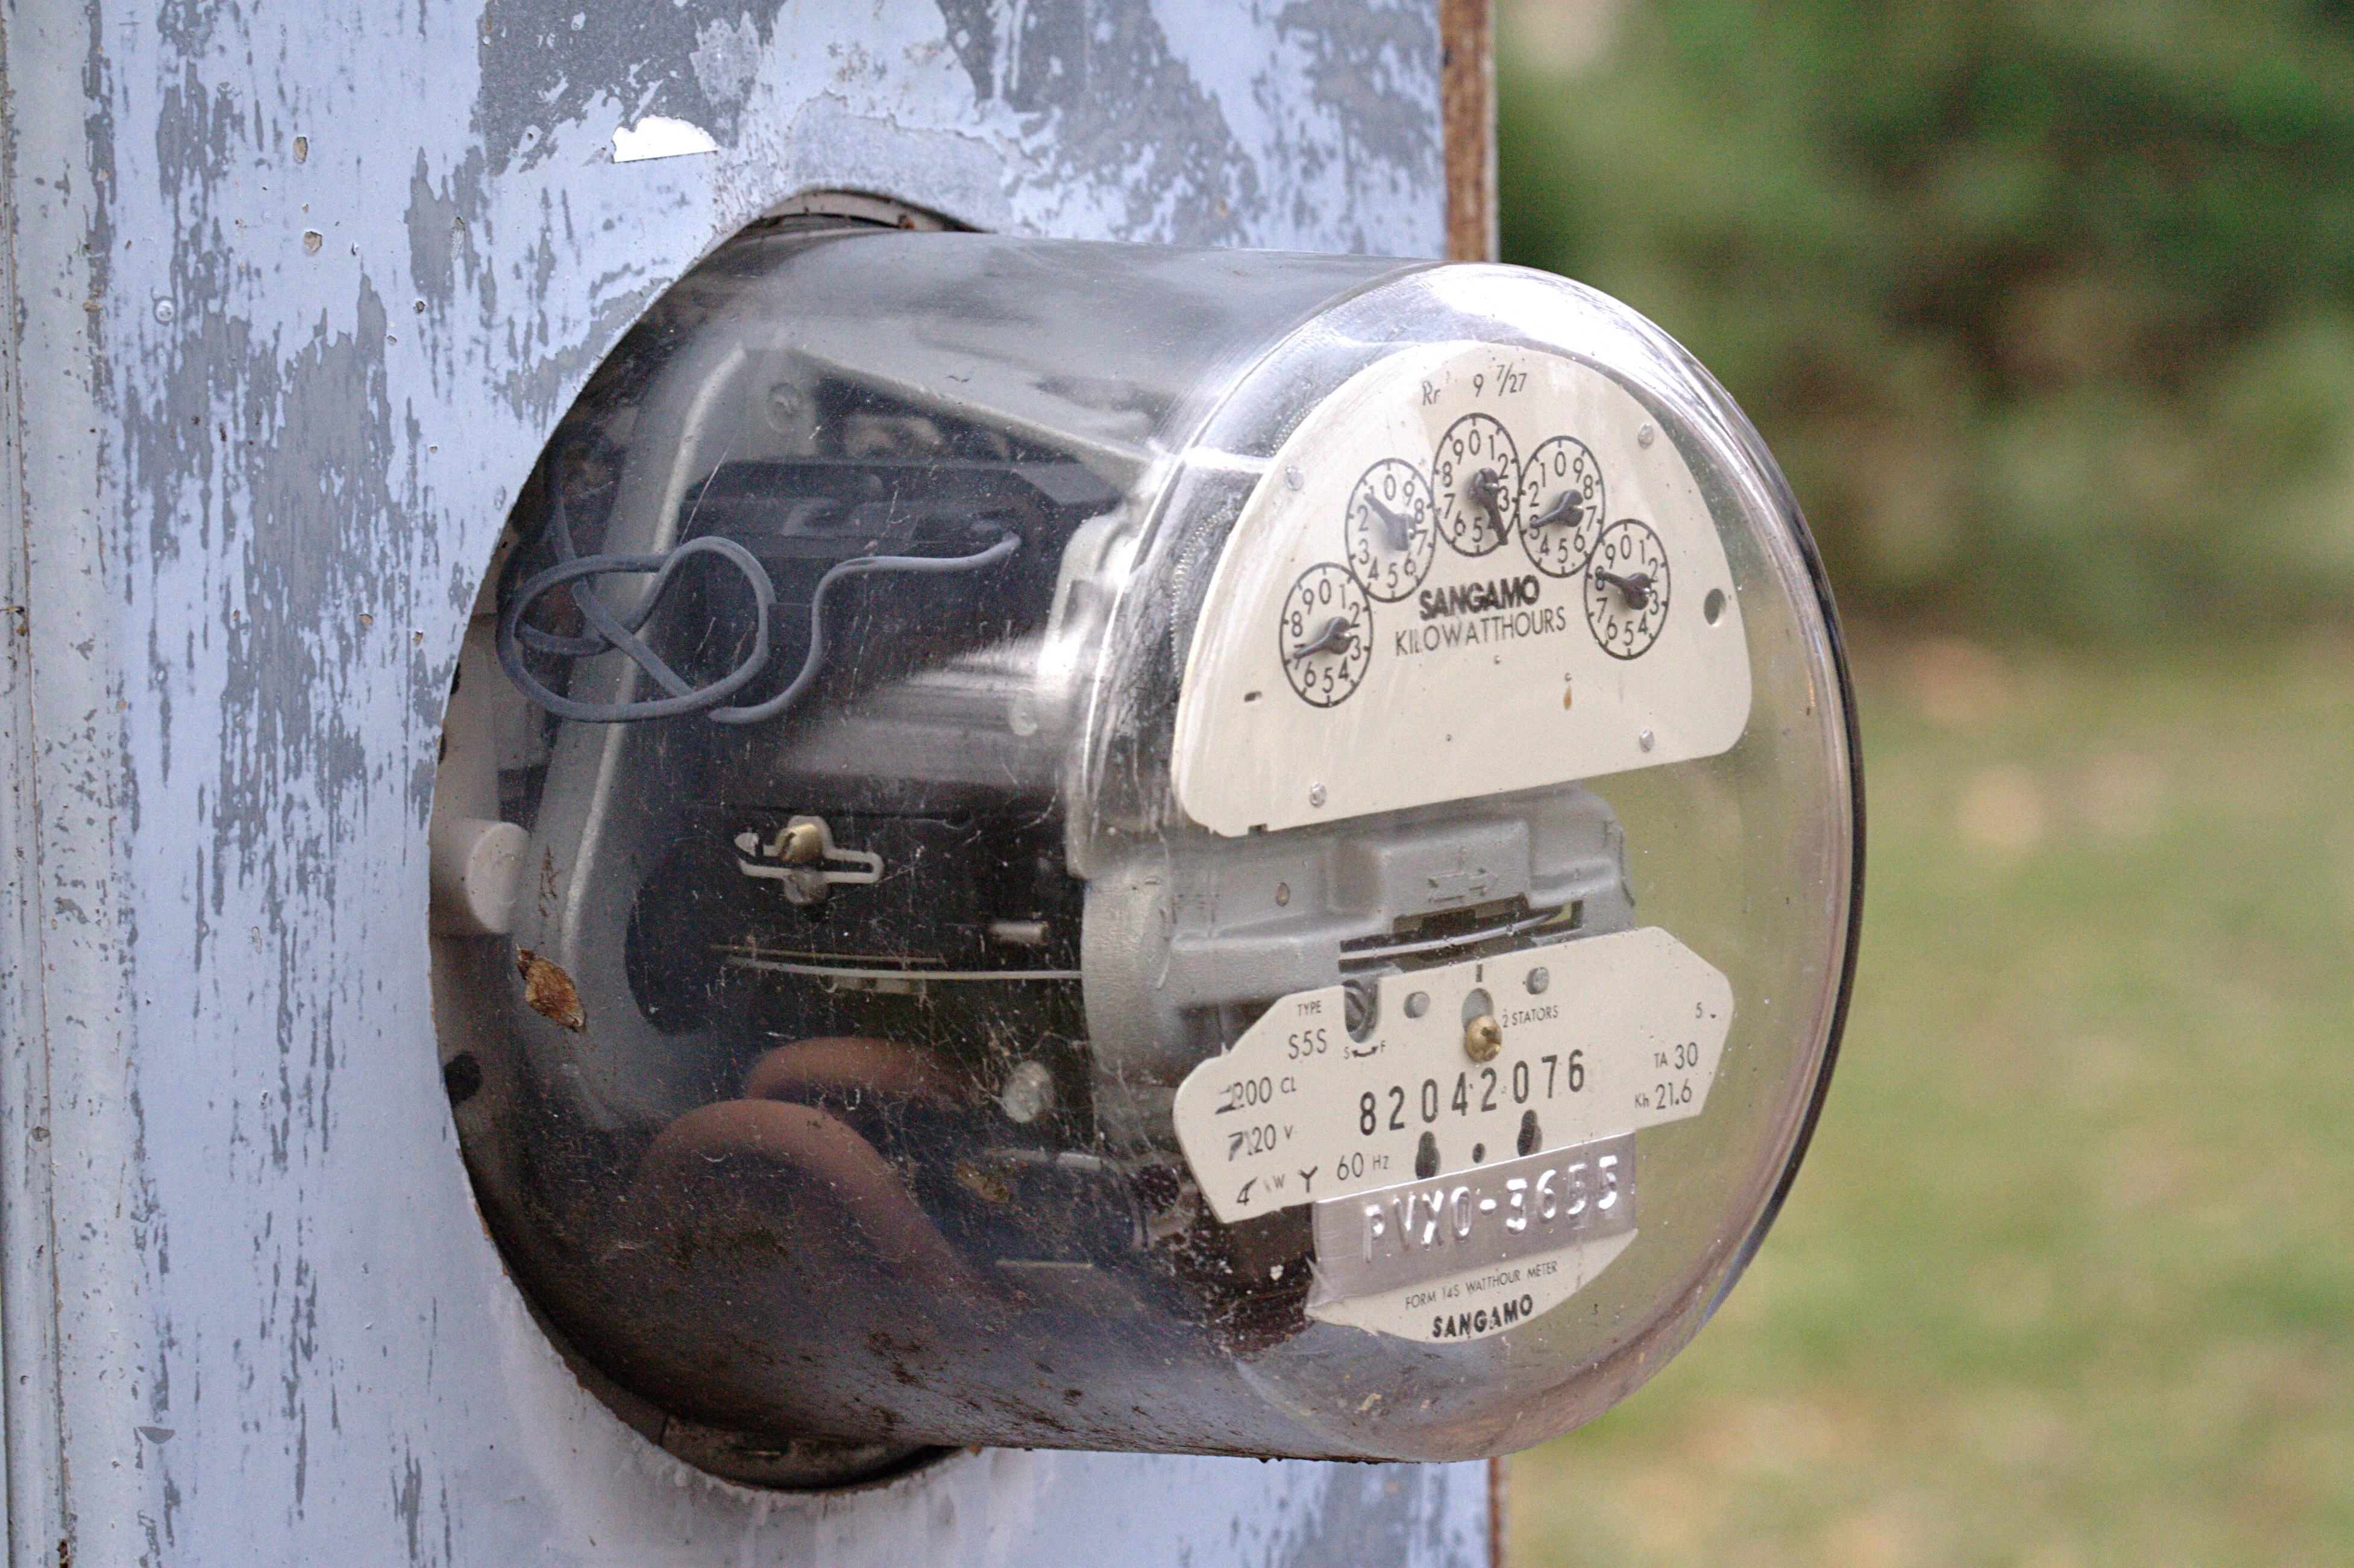
\includegraphics[width=5in]{includes/watt_hour_meter}
  \caption{Standard electric meter; photo copyright Beige Alert (Creative Commons).}
  \label{fig:mechanical_meter}
\end{figure}

Standard electric meters were developed decades ago and are still used today, despite many technological advances in the last several years. Additionally, Americans have become accustomed to having access to large amounts of data, but due to the nature of standard electric metering, data regarding the usage of power is severely limited for both the consumer and electric company. 

\begin{figure}[htbp]
  \centering
  \subfloat[MIT Power usage data.\cite{USEIA}]{\label{fig:mit_usage}\includegraphics[width=3in]{includes/MIT_Energy_Consumption}}\ 
  \subfloat[Energy cost projections.\cite{Cost_Kilowatt}]{\label{fig:energy_cost}\includegraphics[width=3in]{includes/Energy_Cost}}
  \caption{Power usage and cost metrics.}
  \label{fig:power_usage_and_cost}
\end{figure}

Both usage and cost of electricity continue to increase, see figures \ref{fig:mit_usage} and \ref{fig:energy_cost} respectively, causing consumers and providers to look for ways to become more efficient. With more data about electric usage available, both parties can find inefficencies and take action as appropriate. Currently, few simple or inexpensive solutions exist, and most only address part of the whole problem, giving some information to the consumer and none to the power company or vice-versa.

%% Customer base, from business plan s. 3.5
\subsection{Customer Base}
The target market for the entire PICA system comprises both electricity
producers and electricity consumers, as set forth by the nature of the
subsystems. As the power companies supply and own the electricity meters
attached to the buildings to which they supply power, the PICA E-meter appeals
only to the market of electricity-producing companies. The other two subsystems,
the solid-state breakers and base station, target the power-consuming audience,
as the devices will assist in monitoring power flow inside the building, where
the power company has no presence. As these two markets are essentially
exclusive in both membership and interest in the PICA subsystems, the E-meter
will be able to function independently of the other consumer-targeted
subsystems, and vice versa.

\subsubsection{Power Companies} % Fixed
As power companies currently distribute the whole-building metering hardware
that determines how much energy their customer used, the E-meter clearly targets
power companies. In fact, the power companies own the power-measuring hardware
external to the buildings to while they provide power, so only they may replace
or upgrade those devices. At present, power companies send trained meter-readers
to read the data from most traditional power meters under their control. The
PICA E-meter subsystem aims to improve on this process by automatically sending
the measurements to the power company using a means and protocol selected by the
particular company. While this will require some hardware customization for each
company, the volume of company-specific production should allow the cost to
develop the design to spread into a small per-unit cost. 

The PICA E-meter subsystem also provides numerous more measures of power than
the simple spinning-dial meters. For example, the E-meter will measure the
frequency and the RMS voltage of the incoming supply lines, which help indicate
the overall quality of power delivered to the customers in the area. This
information may also help diagnose any observed issues with power delivery
without dispatching a worker to take measurements by hand. In this way, power
companies using the PICA E-meter can improve the quality of the service they
provide and can save on the labor costs associated with making a site visit. 

\subsubsection{Power Consumers}
Although the power company's customers cannot modify the metering panel
installed by the power company, they are free to modify the other power
distribution components inside their own buildings. The solid-state breakers
fall into this category, and provide previously unavailable measurements
regarding power consumption and its location within the building. However, as
these breakers will replace the pre-existing breakers inside the building, the
consumer must be convinced that using the PICA system is worth the trouble and
cost of replacing the mechanical circuit breakers with the more feature-rich
PICA breakers. To this effect, the most receptive market for the solid-state
breakers includes homeowners and building managers who are curious or concerned
about power usage inside their building. That is, the people for whom this
information can inspire a meaningful change in practice will likely become the
first adopters of the subsystem. 

The product may also gain a following as an alternative to mechanical breakers
in during the construction of a new home or building. This would likely require
that the product already have a proven history of reliability and safety, so the
previous group of cost- or environmentally-concerned individuals might have to
adopt the produce first. If the PICA solid-state breakers become an alternative
during construction, the net cost to the user will be lessened, as the
building-to-be will not have any pre-existing breakers to discard or replace. 

The base station may apply to either of these two consumer groups, as its
primary purpose is to manage and interface with the other systems. It does not
specifically require the solid-state breakers or the E-meter, but provides
little value in a building without any installed PICA systems. The base station
exists solely to manage and collect data from other PICA subsystems, as well as
format and display these measurements, so its target audience consists of power
consumers whose buildings use the E-meter, the solid-state breakers, or both.
 
\subsection{About Us}
\begin{figure}[htbp]
  \centering
  \includegraphics[width=6in]{includes/IMG_0865}
  \caption{Team PICA left to right: Amy Ball, Kendrick Wiersma, Nathan Jen, and Avery Sterk.}
  \label{fig:team_picture}
\end{figure}
\textbf{Amy Ball}: Amy, from Wayland, Michigan, works as an intern at Johnson Controls as part of the Systems Engineering Team. She brings good communication skills, circuit-building experience, and presentation skills to the project. Originally her section was the solid-state breakers, but the team decided to use solid-state relays for the breaker purposes. After which her new task was to build all of the power supplies for the project. Additionally, she was assigned to identify a method to match outlets to breakers.


\textbf{Kendrick Wiersma}: Kendrick works as an intern at Raytheon in the Electronics Center, where he performs embedded system design and verification in \ac{VHDL}. Kendrick hails from Tucson, Arizona where he was born and raised. He brings real-world project experience and experience working with embedded hardware and software to the team. Kendrick leads the development of the E-meter, which primarily measures total power consumption, reporting data to the power company and the PICA base station.


\textbf{Nathan Jen}: Nathan, from Kentwood, Michigan, has worked at Amway on the production floor and has gained involvement with club leadership at Calvin College. He will be graduating with an Engineering degree, Electrical and Computer Concentration. He brings leadership experience and a good understanding of how smaller elements of a system fit together as a whole. After graduation, Nate has accepted a position with American Electric Power, working at the D.C. Nuclear Plant in Bridgeman, Michigan. His section of the project is the monitoring of individual circuits and some of the control logic for the breakers. 


\textbf{Avery Sterk}: Avery comes from Santa Clara, California where he worked as an intern at the SLAC National Accelerator Laboratory doing CAD design. He will be graduating with a degree in Engineering Electrical and Computer Concentration and a Math minor. He brings varied experience with software design and implementation to the project. Avery is the technical lead on the base station, especially providing the primary user interface and designing embedded software. Additionally Avery became the software lead on the E-Meter after changing the focus of the base station component of the project.
 
\subsection{About the Course}
Taken from the Calvin College course catalogue:
\begin{quote}
This course takes place over two semesters in the senior design project sequence. For the first semester course (Engineering 339), emphasis is placed on design team formation, project identification, and production of a feasibility study. Students focus on the development of task specifications in light of the norms for design and preliminary validation of the design by means of basic analysis and appropriate prototyping. Lectures focus on integration of the design process with a reformed Christian worldview, team building, and state-of-the-art technical aspects of design. Interdisciplinary projects are encouraged. Prerequisites: Concurrent registration in the seventh semester of the model program for a particular concentration or permission of the instructors; developing a Christian mind and philosophical foundations.

For the second semester in the senior design project sequence (Engineering 340), emphasis is placed on the completion of a major design project initiated in Engineering 339. This project should entail task specifications in light of the norms for design by means of engineering analysis and an appropriate prototype focused on primary functionality. A final presentation is given at the May Senior Design Night Banquet. Lectures continue to focus on integration of the design process with a Christian reformed world-view, team activity, and state-of-the art technical aspects of design.
\end{quote}
% Scheduling section, by Avery
\section{Scheduling}
The team initially created a Gantt chart to establish a timeline for the
project and display the critical path for the tasks in the project. As the
team decided to first focus on the Smart Breakers, they elaborated the
different elements of that subsystem first. Additionally, the team included
the known class deadlines for assignments into the Gantt chart to visualize
how much time to allot to those assignments. These charts are included in
appendix \ref{sec:gantt_charts_appendix}.

In practice, however, the team's usage of the Gantt chart dimished soon
after its introduction. As such, the chart remains essentially the same now
as it was in late October, with many tasks and sub-tasks yet to be filled
and assigned. While the attention paid to the Gantt chart waned, the
emphasis of schedules in team meetings increased. The team would use its
meetings to review the upcoming duedates and assign them to individuals,
much in the same way that the Gantt chart would be used.

Additionally, the team created their own website on Google Sites to provide
a flexible scheduling system independent of Microsoft Project, which is
limited to Engineering computers. After each weekly status update meeting,
during which individuals acquired tasks, Nathan would update the website's
task list to reflect the new assignments and their due dates. While this
system does not allow for the critical-path linkages that Gantt charts
feature, this customizable task list can include any information desired,
such as priority, status, and reviewing information. In some instances, the team mistakenly assigned a small task for the duration of the week, leading to wasted time and letting the project fall behind.

The class deadlines posted on Moodle kept the team focused on some of the long-term goals. Focusing on the larger time scale helped the team allocate more proportionally equal amounts of time for each component of a system. This allowed the team to design by choosing components to fit the system, instead of modifying the system to fit the components.
% System_Overview.tex
% replaces Problem Definition and Customer Base
\section{System Overview}

%% System Requirements from beginning/PPFS
%\subsection{System Requirements -- TBD}   % not including this here since we have a full section just for requirements
%To be included...

%% System block diagram
\subsection{System Block Diagram}
\begin{figure}[htbp]
  \centering
  \includegraphics[width=\textwidth]{includes/PICA_System_Diagram_B}
  \caption{System block diagram}
  \label{fig:system_block_diagram}
\end{figure}

%% System Explantion
\subsection{System Explanation}

The full PICA system consists of the e meter, base station, smart breakers and power supply. The system was designed to minimize dependencies between subsystems, allowing the user to choose which information they want without paying for more than that. The fact that the power company and homeowner both have an interest in the PICA system drove much of this decision. As two customers with different requirements, neither party would want to pay to provide the other with information that isn't useful to the first. The team wanted both parties to have information if they wanted it without forcing unwanted costs on one party or the other. The team later decided that designing for the power company was not feasible. However, keeping the subsystems as independent as possible allows for continued development with the power company's interests in mind should another team work on the project later.

The e meter measures power for the entire building and provides information to the power company. The built in display allows the e meter to operate and provide information completely independently of the base station, although the Xbee connection allows viewing of the information through the base station if desired. The e meter is dependent on the power supply.

The base station is targeted at the homeowner, providing a simple and easy way of viewing information collected by other parts of the system. While the e meter and breakers are not required for the base station to run, it would have no information to provide, and would therefore be useless. Because the base station provides no controls for the other subsystems, it is not required for the other subsystems to operate properly. The base station is not dependent on the power supply. After a lot of work on the base station, the team decided to focus on the e meter and smart breakers and use a standard computer in place of the dedicated base station for prototyping and testing.

The smart breakers provide circuit breaker level information to the homeowner, in addition to providing the same functionality as standard air-gap breakers. The smart breaker's only means of displaying the information is through the base station, so to provide useful data the smart breakers are dependent on the base station. However, the smart breakers still function as breakers without the base station. This is important so that a problem with the base station doesn't shut off power to all of the smart breaker circuits. The smart breakers are also dependent on the power supply.

The power supply provides power to the E-Meter and Smart Breakers and is placed so that it is still able to power everything when all of the breakers are shut off. This is important because the smart breakers' default state is off and won't turn on until they have power, so if the smart breaker came before the power supply, the system would never turn on. 

%% Testing
\subsection{Testing}
Once each subsystem passes its respective verification plan, the three PICA systems can begin integration testing. The system level integration testing verifies that all systems are capable of talking to one another under normal operating conditions.
\subsubsection{Simple Talk Test}
This test verifies that all systems are capable of talking to one another. Begin by placing both the smart meter and the breaker in a situation where they are guarenteed to talk, such as monitoring an active load. Attach a computer to each device, verifying that in fact they are correctly sending data. Once each system has been verified to be operational, attach Xbee radio cards to the prototype boards and a computer console to the base station. Verify that data transmitted from each device is received by the base station computer. The team expects that data received at the base station will be identical to data seen leaving each device.

\subsubsection{Simple Command Test}
This test verifies that the base station is capable of sending various commands to the individual subsystems. After all systems have been powered on and placed in an operation state, send the `q' command out across the Xbee network. This should result in both systems halting in an expected fashion. The E-Meter should cease taking measurements and blank the screen while the Smart Breaker changes to the Off state. At this time, both should stop talking.

Continue this test by trying this command an additional time, but specifying which subsystem should respond to the command. Test the E-Meter and Smart Breaker individually, each time sending the `q' command. The response should be the same, but only the device specified should halt.

\subsubsection{Complex Command Test}
Repeat the previous test, using more complex commands asking for specific information. Commands can be seen in the table \ref{tab:pica_system_commands}.
\begin{table}[htbp]
  \centering
  \begin{tabular}{|c|p{2in}|}\hline
    Command & Behavior \\\hline\hline
    q     & Kills the system \\\hline
    b\#    & Specifies a breaker to command\\\hline
    m     & Specifies the command is for the E-Meter\\\hline
    v [\#] & Specifies that voltage should be reported. An optional number is allowed for sending to the meter to select which phase.\\\hline
    i [\#] & Identical to v except returns current.\\\hline
    p [\#] & Identical to v except returns power.\\\hline
    wh    & Returns the accumulated watt-hours.\\\hline
    s     & Used in conjunction with a breaker to return its status.\\\hline
  \end{tabular}
  \caption{PICA System commands.}
  \label{tab:pica_system_commands}
\end{table}
As a result of sending any one of these commands, either all or the specified system should return the data requested.

\subsubsection{Web Interface Test}
Verify that the system is properly reporting data to the web interface and rerun all tests through the web interface command line. Results should match those seen in previous tests.
%Basic Xbee tests proved it is a viable option for communication between subsystems.

%Some testing was completed, using the standard computer and e meter. [Pictures of perl 'base station' should go in this section]

%Testing between the smart breakers and base station need to be completed once the smart breakers are functional.
%which isn't really true since we could have generated numbers with the Arduino and just used that...

%% Future Work
%\subsection{Future Work -- TBD}
\section{Requirements}

\subsection{Base Station Requirements}\label{sec:base_station_reqs}
All requirements under this heading are to be assumed to be of the base station (``the system'') unless explicitly stated otherwise.

\subsubsection{Functional Requirements}
\begin{outline}[enumerate]
\1 Shall be capable of upgrading its software and firmware upon administrator requests.
\1 Shall be capable of connecting with other PICA sub-systems over a pre-defined and pre-arranged communications protocol.
 \2 Shall receive and store power usage measurements from connected PICA systems.
  \3 These measurements will be taken at a frequency that does not exceed the established bandwidth of the chosen protocol.
  \3 These measurements will be summarized or discarded (at the user's selection) when the storage space of the system nears its capacity.
 \2 Shall receive and store events and alerts from connected PICA systems.
  \3 The nature of these events shall be determined by each individual system, but shall be communicated to the base station in a standardized format.
  \3 The system shall organize these events internally and display them to the user.
 \2 Shall function as a \ac{NTP} server for connected PICA systems.
 \2 Shall receive and record event log information from connected PICA systems.
\1 Shall be capable of connecting to a \ac{LAN}.
\1 Shall be capable of using settings that the user selects.
 \2 Shall be capable of recognizing an invalid setting.
 \2 Shall be capable of reverting to a default setting when the user setting is not valid.
\1 Shall be capable of displaying the most recent measurements from the connected PICA systems.
\1 Shall be capable of displaying the status of the connected PICA systems.
 \2 Status shall include whether the connected system is in an error state.
 \2 Status shall include the time since the last observed error state, if applicable.
 \2 Status shall include the nature of the last error, if communicated.
\1 Shall be capable of giving an authenticated base-station adminstrator similarly-privileged administrative access to connected PICA systems.
 \2 The extent of this access shall be deteremined by the individual PICA systems.
 \2 The base station shall inform the administrator when the remote administrative access is rejected or unavailable.
\1 Shall be capable of distributing system updates for connected PICA systems.
 \2 Shall be capable of sending update data and images to the appropriate subsystems.
 \2 Shall identify whether or not the connected PICA systems require updating.
\1 Shall be capable of giving debugging and troubleshooting output.
 \2 Shall display simple status indication using \acp{LED}. (See \ref{sssection:base-station-ui-reqs})
 \2 Shall present more detailed debugging and troubleshooting information over a dedicated RS-232 connection.
\1 Shall be capable of actively notifying the power-company and consumer.
\end{outline}

\subsubsection{Behavioral Requirements}
\begin{outline}[enumerate]
\1 Shall store user-defined configuration in non-volatile media.
 \2 Shall initialize this configuration using a pre-defined default configuration.
 \2 Shall load the default configuration if the user-defined configuration is unavailable.
  \3 This includes the user-defined configuration being absent.
  \3 This includes the user-defined configuration containing invalid data.
\1 Shall include a backup firmware in the event of a failed firmware upgrade.
 \2 Firmware upgrade success or failure shall be determined by comparing checksums of the firmware to be written and the firmware present after writing.
 \2 The backup firmware shall be engaged if the system fails to boot from the first firmware.
\1 Shall store critical event logs from connected PICA systems in a non-volatile media.
\1 Shall host a webpage to display system information when browsed over the \ac{LAN} connection.
\1 Shall store its software in non-volatile media.
\1 Shall run an operating system to manage hardware, device drivers, and connections to connected PICA systems.
\1 Shall use a defined communication protocol to communicate with connected PICA systems.
\end{outline}

\subsubsection{Software Requirements}
\begin{outline}[enumerate]
\1 Shall include and run an upgradable \ac{OS}.
\2 The \ac{OS} shall include the drivers necessary to operate the system hardware.
\2 The \ac{OS} shall include the protocols necessary to connect to PICA sub-systems.
\1 The \ac{OS} shall have an administrator-privileged user who may change the configuration of the system and of connected PICA systems.
\1 The \ac{OS} shall give the system owner access this administrator-privileged user account.
 \2 The \ac{OS} is not required to give such access to connected systems that are not owned by the owner of the base station system (such as those owned by the power company).
 \2 The \ac{OS} shall authenticate that the user requesting administrator access is authorized to do so using a means configured during system installation.
\1 The \ac{OS} shall include the protocols necessary to connect to an existing \ac{LAN}.
 \2 The \ac{OS} shall include a \ac{DHCP} client.
 \2 The \ac{OS} shall support manual \ac{LAN} connection configuration.
\1 The \ac{OS} shall control the system connectivity hardware to prevent unwanted devices, such as those owned by other customers, from being connected to the system.
 \2 The \ac{OS} shall distinguish between wanted and unwanted systems as defined by administrator selection.
  \3 By default, ZigBee connection requests will be rejected until authorized by the administrator.
  \3 By default, \ac{LAN} connection requests will be trusted unless disallows by the administrator. 
 \2 The \ac{OS} shall record connection requests from unwanted devices and display them to the administrator.
\1 Shall include and run \ac{HTTP} server software to provide the web interface.
\1 Shall include the necessary tools to download and apply software and firmware updates.
\end{outline}

\subsubsection{Hardware Requirements}
\begin{outline}[enumerate]
\1 Shall include a power supply to power the system from line voltage during regular usage conditions.
\1 The power supply shall tolerate moderate expected fluctuations in input voltage from a standard power outlet.
 \2 The power supply is not required to tolerate incorrect voltage input (240V instead of 120V, etc.)
 \2 The power supply is not required to tolerate voltage spikes as may be associated with electrical storms.
\1 Shall include an internal power storage device to allow the system to perform necessary data storage immediately after a power failure.
\1 Shall have adequate \ac{RAM} to contain system software, cache data from other PICA devices, and cache data to send to other PICA devices without requiring a cache flush more than once per minute.
\1 Shall have a processor to execute the system software and process data from connected PICA devices.
 \2 The processor must have sufficient processing speed to process the incoming data from other PICA devices at a rate greater than the rate of data incoming.
 \2 The processor must be able to perform all necessary mathematical operations without a co-processor.
\1 Shall have an Ethernet controller for connecting to a \ac{LAN}.
\1 Shall have an RS-232 controller for debugging and troubleshooting the system.
\1 Shall have ZigBee connectivity hardware for communication with other PICA systems.
\1 Shall have non-volatile storage dedicated to storing system firmware.
 \2 Shall have a re-writable non-volatile storage device to contain boot firmware.
 \2 Shall have a separate non-volatile storage device to contain backup firmware to use in the event of boot failure.
\1 Shall have non-volatile storage sufficient to store system software.
\1 Shall have non-volatile storage sufficient to store recorded events and short-term consumption history for up to a period of 3 years.
\end{outline}

\subsubsection{User Interface Requirements}
\label{sssection:base-station-ui-reqs}
\begin{outline}[enumerate]
\1 Shall provide a web interface for viewing collected data over the \ac{LAN}.
\1 Shall provide a web interface for viewing current and predicted pricing information as provided by the power company.
\1 Shall provide a web interface for system administration to an authenticated administrator.
 \2 Shall include an interface for managing updates to the system's firmware and software
  \3 Shall include an interface for displaying the version numbers or codes of the firmware and software currently installed on the base station.
  \3 Shall include an interface for indicating the availability of system updates for the base station.
  \3 Shall include an interface by which the administrator may request that the base station apply its available updates and be informed on whether or not the base station must be rebooted after the update is installed.
  \3 Shall include an interface for indicating the progress of update installation.
 \2 Shall include an interface for managing connections to other PICA systems.
  \3 Shall include an interface for displaying current connections to other PICA systems.
  \3 Shall include an interface for adding, removing, or connections made to other PICA systems.
 \2 Shall include an interface for administration of connected PICA systems.
  \3 Shall include interfaces for managing configurations of connected PICA systems.
  \3 Shall include an interface for deploying software/firmware upgrades to connected PICA systems.
\1 Shall provide a debugging interface over an RS-232 serial connection.
\1 Shall display status indication lights.
 \2 System is connected to power.
 \2 System is connected to other PICA subsystems.
 \2 System is connected to the home network.
 \2 System has encountered an error.
  \3 Error light shall trigger if a connection to another PICA system is lost and cannot be recovered within 30 seconds.
  \3 Error light shall trigger when the storage medium contains less than $5\%$ free space.
  \3 Error light shall trigger when the storage medium's file system cannot be mounted.
   \4 This includes the storage medium being physically absent.
   \4 This includes the storage medium being corrupt.

\end{outline}

\subsubsection{Power Requirements}
\begin{outline}[enumerate]
\1 Shall be powered from a standard 120V wall outlet.
\1 Shall have a \ac{DC} power supply to power internal components.
\1 Shall have a backup power supply to enable the system to save all measurements residing in memory to the non-volatile storage medium.
\1 Shall require less than 10W to operate.
\end{outline}

\subsubsection{Codes and Compliances}
\begin{outline}[enumerate]
\1 Shall have a polarized electrical plug if the power supply features an an off-on control switch.
\1 Shall restrict \ac{EM} radiation to comply with \ac{FCC} Title 47 Part 15.
\end{outline}

\subsection{Smart Breaker Requirements}\label{sec:ssb_reqs}
All requirements are to be assumed to be of the solid state breakers (``the system'') unless explicitly stated otherwise.

The breaker subsystem must be capable of two major functions; it must protect the connected circuit when a specified threshold is exceeded, and it must pass information to and from the user interface, either directly or through another subsystem.

\subsubsection{Functional Requirements}
\begin{outline}[enumerate]
\1 Shall be capable of completely disconnecting, either physically or virtually, the power delivered to the connected circuit.
\1 Shall provide two-way communications to the base station through the \ac{MCU}.
\2 Shall provide power usage information, including at a minimum, instantaneous voltage and current of the connected circuit.
\2 Shall be capable of providing on/off status of the breaker.
\2 Shall be capable of turning breakers on and off when requested by the base station.
\1 Shall be capable of detecting power sags, brownout conditions and blackouts.
\2 The \ac{NPC} defines sag as ''80\% to 85\% below normal [voltage] for a short period of time,'' \cite{natpow}. For project uses, this is below 100V. The team defines ``a short period of time'' to be for three cycles to ten cycles, based on information given in \cite{VoltSag}. The \ac{NPC} defines a brownout as ``a steady lower voltage state,'' \cite{natpow} Blackouts are defined by the \ac{NPC} as ``as zero-voltage condition that lasts for more than two cycles,''\cite{natpow}.
\1 Shall store up to a minute of gathered information for at least five minutes in on-chip memory for transmission to the \ac{MCU}.
\1 Shall package the stored information for transmission to \ac{MCU}.
\1 Shall be capable of turning off circuits individually.
\1 Shall stop current flow to a circuit when it exceeds a specified threshold.
\1 Shall be capable of being reset when stopped, without requiring new parts such as fuses.
\end{outline}

\subsubsection{Behavioral Requirements}
\begin{outline}[enumerate]
\1 Shall initialize all components by writing from non-volatile storage to all necessary registers when power is restored to the circuit.
\1 Shall report all system events that are not part of standard operation to the critical event log.
\1 Shall measure voltage levels in the connected circuit.
\1 Shall measure current flow in the connected circuit.
\end{outline}

\subsubsection{Hardware Requirements}
\begin{outline}[enumerate]
\1 Shall use non-volatile storage to store data when the system is without power.
\1 Shall be capable of managing its own data and functions.
\end{outline}

\subsubsection{User Interface Requirements}
\begin{outline}[enumerate]
\1 Shall have an external interface that is understandable by the average consumer.
\1 Shall provide a way to control the breakers independent from the base station.
\1 Shall encase all circuitry except user interface controls (buttons, switches) so that they cannot be tampered with without breaking the casing.
\end{outline}

\subsubsection{Power Requirements}
\begin{outline}[enumerate]
\1 Shall be powered by line-voltage.
\1 Shall be powered such that interrupting the circuit does not cause the breaker control circuitry to lose power.
\end{outline}

\subsubsection{Physical Requirements}
\begin{outline}[enumerate]
\1 Shall have dimensions less than or equal to 1in x 3in x 4in for a single breaker or 2in x 3in x 4in for a breaker pair.
\2Dimensions are determined by the standard size of a mechanical breaker, so that smart breakers may be interchangeable with conventional residential or commercial mechanical breakers.
\1 Shall not weigh more than one pound.
\2 Weight is determined by the average weight of a standard mechanical breaker \cite{homedepot}, so that smart breakers may be interchangeable with conventional residential or commercial mechanical breakers.
\1 Shall accommodate wire sizes from 14-4 Cu to 12-8 Al.
\2 Wire size is based on the average size wire used with standard mechanical breakers \cite{homedepot}, so that smart breakers may be interchangeable with conventional residential or commercial mechanical breakers.
\end{outline}

\subsubsection{Safety Requirements}
\begin{outline}[enumerate]
\1 Shall protect everything connected to the circuit from current exceeding a specified threshold by providing circuit interruption.
\1 Shall have safety hazards clearly marked and visible from outside the system.
\1 Shall safely isolate high-voltage areas so that they provide no more threat than a standard wall outlet.
\end{outline}

\subsubsection{Codes and Compliances}
\begin{outline}[enumerate]
\1 Shall be compliant with \ac{ANSI} C12.19 \cite{ANSIC1219}.
\1 Shall be compliant with \ac{ANSI} C12.21 \cite{ANSIC1221}.
\1 Shall be compliant with \ac{FCC} Title 47 Part 15 \cite{FCC}.
\end{outline}

\subsection{E Meter Requirements}\label{sec:e_meter_reqs}
All requirements are to be assumed to be of the electric panel meter (``the system'') unless explicitly stated otherwise.

\subsubsection{Functional Requirements}
\begin{outline}[enumerate]
\1 Shall continuously monitor the power used from either a single-phase or a multi-phase installation.
\1 Shall store power usage data locally, to be transmitted back to the base station at regular intervals.
\1 Shall by default display instantaneous and historical power usage data on an \ac{LCD} module integrated into the electric panel.
\1 Shall provide two-way communication with the \ac{MCU} to report usage data.
\1 Shall be capable of detecting a brownout condition and storing critical data before shutting down.
\1 Shall be capable of restarting and restoring stored data after a brownout condition.
\1 Shall be capable of detecting any tampering, such as opening the sealed metering unit, and transmitting a tamper message to both the power-company and the consumer.
\1 Shall monitor current flow through the main service lines for automated meter reading.
\1 Shall monitor voltage levels on the main service lines for automated meter reading.
\1 Shall control the service shutoff switch by receiving and validating a service shutoff message from the power-company.
\1 Shall provide a method for controlling the service shutoff switch from a local interface.
\1 Shall provide an interface for 3rd party meters, such as gas, water, or other utility meters to report data over the PICA network.
\1 Shall support on-demand reports from the power company via the Zigbee network or the user via the PICA web interface of power usage, energy consumption, demand, power quality and system status.
\1 Shall support bi-directional metering and calculation of net power usage to support alternative energy generation systems.
\1 Shall support automatic meter reads.
\1 Shall analyze the voltage flicker, logging a warning when the flicker exceeds 20\% of the stated $117V_{RMS}$. 
\1Shall meter reactive power consumption, logging data for billing purposes.
\end{outline}

\subsubsection{Behavioral Requirements}
\begin{outline}[enumerate]
\1 Shall, in the event of wireless link loss; attempt to re-establish the wireless link.
\1 Shall, in the event of a wireless link loss, revert to stand-alone mode, storing data internally until internal storage is full, at which point the system will begin overwriting the oldest data with the newest data.
\1 Shall, in the event of a wireless link loss, notify the user via the \ac{LCD} display.
\1 Shall perform a built-in self-test upon system boot up to verify onboard storage integrity and to verify proper operating software.
\1 Shall, in the event of a brownout, save all volatile information to non-volatile storage space.
\1 Shall be capable of detecting corrupted data, via parity bits, when brought out of a brownout condition.
\1 Shall log all events processed into the following four categories: 
\2 critical: messages requiring immediate attention. 
\2 error: messages requiring attention and may affect system functionality. 
\2 warning: messages that require attention but do no impact system functionality.
\2 note: messages that require no attention but provide verification of proper operation. 
\1 Shall report all events to the PICA base station.
\1 Shall report to the power-company as specified by event criticality.
\1 Shall have dedicated non-volatile storage for all critical settings and configuration data.
\1 Shall compute the total power used in kilowatt-hours.
\1Shall be capable of receiving messages from the power-company, providing the user with the current cost of a kilowatt-hour.
\1 Shall use 128-bit \ac{AES} encryption for all messages transmitted outside of the device. 
\1 Shall report the total amount of outage time to both the power company and the PICA base station. 
\1 Shall date-stamp all detected outages with the date, time, and duration of the outage.
\end{outline}

\subsubsection{Software Requirements}
\begin{outline}[enumerate]
\1 Shall verify system firmware on boot up.
\1 Shall periodically, minimum once per day, perform a system check to verify the health and status of the system.
\1 Shall perform an on-demand system health and status check as demanded by the PICA base station or the power-company.
\1 Shall contain sufficient non-volatile storage for all system configuration settings.
\1 Shall be updateable through the power-company wireless interface.
\1 Shall be capable of properly recovering from a failed software update.
\1 Shall give authorized access to components of the system configuration as appropriate to the power-company and consumer.
\1 Shall notify the power-company and the PICA base station once service has been restored containing the time of restoration and a voltage measurement.
\1 Shall have a unique IPv6 address for the power-company mesh network.
\1 Shall have a unique IPv4 or IPv6 network address for the local home-area-network. 
\1 Shall receive an \ac{NTP} message from the PICA base station to set the hardware clock. 
\1 Shall synchronize the hardware clock with the base station time once per day. 
\1 Shall support on-demand hardware clock synchronization via the PICA base station web interface.
\end{outline}

\subsubsection{Hardware Requirements}
\begin{outline}[enumerate]
\1 Shall be completely enclosed in a weatherproof case, tolerant of extreme temperature differences. 
\1 Shall be completely \ac{AC} coupled against transient \ac{AC} voltages. 
\1 Shall be mounted in the same location as a standard power meter. 
\1 Shall provide non-volatile storage.
\1 Shall be grounded.
\1 Shall provide a hardware system clock, set by the software and synchronized with the PICA base station.
\end{outline}

\subsubsection{User Interface Requirements}
\begin{outline}[enumerate]
\1 Shall have a 160-segment \ac{LCD} display module, viewable from outside the electric panel.
\1 Shall be capable of interfacing with a web-based application for stand-alone configuration.
\1 Shall provide push-buttons for changing the viewing contents on the display module between metering and system status views.
\end{outline}

\subsubsection{Power Requirements}
\begin{outline}[enumerate]
\1 Shall be capable of operating from line-voltage.
\1 Shall be powered from before the master breaker, preventing the meter from losing power when the master breaker is switched off.
\end{outline}

\subsubsection{Safety Requirements}
\begin{outline}[enumerate]
\1 Shall meet or exceed safety requirements for devices inside an electric panel. 
\1 Shall provide a grounding point to ground the system when installed. 
\1 Shall be protected against the elements. 4. Shall safely isolate high-voltage areas.
\end{outline}

\subsubsection{Codes and Compliances}
\begin{outline}[enumerate]
\1 Shall be compliant with \ac{ANSI} C12.19.
\1 Shall be compliant with \ac{ANSI} C12.21.
\1 Shall be compliant with \ac{FCC} Title 47 Part 15.
\end{outline}

\subsection{Power Supply Requirements}
All requirements under this heading are to be assumed to be of the power supply (``the system'') unless explicitly stated otherwise.
\begin{outline}[enumerate]
\1 Shall be 78\% efficient.
\2 This efficiency was chosen, because it is what SMPS were generally.
\1 Shall power 2 ADE devices.
\1 Shall provide 5VDC +/- 5\%.
\1 Shall provide $2\milli\ampere$, $3\milli\ampere$ (total $5\milli\ampere$) plus a Safety factor.
\2 A safety factor can be efficient as 1.0001x.
\1 Shall also power an FPGA that will control these chips in a production-scale design at 5VDC $\pm5\%$.
\2 While the exact requirement for the FPGA are unknown the current was chosen much higher than probably needed in order to make sure the power supply would not need to be changed to provide more power.
\1 Shall have a ripple voltage of less than $~1\%$.
\1 Shall be isolated from mains supply by a high frequency transformer $~60Hz$.
\1 Shall be small and not exceed $4\inch^3$.
\1 Shall not be hot enough to where heat sinks are required.
\end{outline}

\section{Design Goals}
\subsection{Provide a physical system that accurately monitors power usage}
Inaccurate information provides no benefit to either the power company or the consumer, despite any added features. Therefore, the system should be as accurate as or more accurate than monitors currently used.

\subsection{Provide manuals for maintenance and general use}
The design team recognizes that no system is perfect and will eventually need maintenance and that most consumers do not have extensive knowledge of electrical systems or components. Providing manuals will assist the consumer in understanding their system and getting the most benefit from it. The design team will look to create a manual that will include an overview of how the system works, how to install and configure the system, and how to maintain the system during the course of normal use. This manual will also contain a troubleshooting guide, support information, liabilities, safety information, and any other pertinent information.

\subsection{Design the system to be modular}
Providing information to both the power company and to the consumer is the main goal of the project, but it is possible that an installation will not include all the subsystems. For example, a consumer may want the consumer-oriented part of the system, while the power company does not want the power-company-oriented subsystem, or vice versa. The modularity goal aims to satisfy all situations without forcing extra costs on any party. To do this, the design team will design the system so that the subsystems providing information to the power company and the subsystems providing information to the consumer do not depend on or require each other.

\subsection{Present power usage information in a way that is understandable to an average consumer}
The goal of the design team is to present the information in an understandable format for the consumer. Because the average consumer does not have an engineering background, the design team would like to display the power usage information in dollars per minute, per hour, per day, per week, per month and per yearly. The system will report these costs in addition to more technical information including voltage, current, power factor and more.

\subsection{Minimize on-site maintenance as much as possible}
In many cases, the consumer calls the power company to fix something as simple as a tripped breaker, and the power companies waste a lot of time just driving to and from the site. The ability to do work remotely allows the power company to minimize this cost. Remotely controlling or monitoring different aspects of the meter also lets the power company quickly assess if a problem still needs attention. Aggravated customers may also become violent towards power-company technicians, so by having remote access, the power company's employees are safer from these threats.
\section{E-Meter}
The E-Meter, short for electricity meter, fulfills the role of monitoring all power consumed for a given customer. The PICA E-Meter exists as a replacement for the standard electricity meter, seen in figure \ref{fig:mechanical_meter}, found outside most homes and businesses. As the PICA E-Meter will replace an already existing piece of technology, the PICA E-Meter must fulfill all the same roles as a traditional power meter. In addition, team PICA seeks to provide extended capabilities, such as wireless meter reading and tamper detection.

Since the average consumer does not actually own the physical metering hardware, this portion of our senior design project targets the electric companies. We hope that by providing more accurate readings, more reliable meters, and more convenience the PICA E-Meter could entice some, if not all of the electric utility providers who still rely on traditional electric meters. The PICA E-Meter should cost less than \$200 each fully assembled. Team PICA currently cannot verify how this price compares to that of a traditional power meter, as they are not available on the open market.

The PICA E-Meter design functions for either 3-phase of 1-phase power, usually found in commercial or residential applications respectively. Both devices share the majority of the hardware, with only a different input board the main hardware functions identically for both applications.

\subsection{Original Ideas}
Early in the project team PICA decided to use a \ac{TI} MSP430 low-power microprocessor. The family of MSP430 devices includes several devices that could perform the necessary tasks, however, the MSP430F471xx family of devices are tailored for metrology. After some investigation the team decided to use an MSP430F47197 microprocessor as the core of the E-Meter. A summary of the specifications for this micrprocssor follows in table \ref{tab:msp430f47197_specs}.
{
\begin{longtable}[c]{|l|l|}
\caption{Specifications for the MSP430F47197\cite{slas626c}\label{tab:msp430f47197_specs}}\\
\hline
\rowcolor{lightgray}
Specification & MSP430F47197\\\hline
\endfirsthead
\caption[]{Continued from previous page}\\

\hline
\rowcolor{lightgray}
Specification & MSP430F47197\\\hline
\endhead
\multicolumn{2}{r}{{Continued on next page}}\\
\endfoot

\endlastfoot

Frequency                    & 16 MHz\\\hline
Flash                        & 120 kB\\\hline
RAM                          & 4 kB\\\hline
GPIO                         & 68\\\hline
Pin/Package                  & 100LQFP\\\hline
LCD Segments                 & 160\\\hline
ADC                          & 7 16-bit Sigma Delta\\\hline
Other Integrated Peripherals & Comparator, DMA, Hardware Multiply, SVS\\\hline
End Equipment Optimization   & Energy Meter\\\hline
Interfaces                   & 2 USCI\_A, 2 USCI\_B\\\hline
Timers                       & 1 Watchdog, 2 16-bit, 2 8-bit\\\hline
\end{longtable}
}
With its included flash, RAM, and onboard peripherals the MSP430 provides a good all-in-one solution on which to base the E-Meter. Along with these features the MSP430 boasted the lowest power consumption of any solution the team examined. A full discussion of one of the alternatives can be found in Team PICA's \ac{PPFS} (pages 34-35)\cite{PICA_PPFS}. Additionally, the team considered using an Arduino for the E-Meter \ac{MCU}, which would then need to interface with an external \ac{ADC}. However, having an integrated solution, where data can simply be read from a register rather than programming and debugging a communications protocol eventually won, taking the Arduino out of the possibilities. The final decision to stick with the MSP430 came when \ac{TI} approved to sample Team PICA a development board, programming pod, and extra processor free of charge. This donation allowed the team to allocate \$150 to another part of the project. 

In order to be compliant with \ac{ANSI} codes C12.19 \cite{ANSIC1219} and C12.21 \cite{ANSIC1221} the PICA E-Meter must display the instantaneous power usage on the local metering unit. For this reason, the E-Meter should have an \ac{LCD} screen displaying the necessary data. After some research, the team found 2 possible display units the SCLCD from SynchroSystems Embedded Computer Design \cite{Synchro} and  the Softbaugh SBLCDA4 from SoftBaugh Inc. \cite{SoftBaugh}. Each of these displays would use the MSP430's internal 160-segment \ac{LCD} driver. As both display units are comparably priced the team chose to use the display from SynchroSystems because they provided a driver written in embedded C along with a backlight kit to make the display more readable. The implementation of this display will be discussed in more detail in the next section.

As a second alternative, the team investigated using a graphic display \ac{LCD} from Newhaven Display International. This particular display, the NHD-C160100DiZ-FSW-FBW, interfaces with the \ac{MCU} over I2C and cost approximately \$20 after shipping. The display featured a 160 x 100 pixel display that could operate on a $3\volt$ supply. Using a display that operates on I2C would only require two I/O pins, rather than the 44 pins required by the SCLCD discussed previously, freeing up 42 pins for more \aa{MCU} I/O devices (such as buttons, data-links, etc.). Because the Newhaven display is a graphic display, the team could draw much more complex graphics, making a much more aesthetically pleasing interface. However, the team would be required to write the entire display driver from scratch, which could be a very lengthy process. Ultimately the team chose to use the SCLCD from SynchroSystems for its shorter development time, and because I/O usage was not a concern. 

\subsection{Hardware Design}
In order to break down the E-Meter into several subsystems Team PICA began with the block diagram seen in figure \ref{fig:simple_e_meter_diagram}.
\begin{figure}[htbp]
\begin{center}
\includegraphics[width=4in]{includes/Simplified_MSP430}
\caption{A simple hardware block diagram of the PICA E-Meter.}
\label{fig:simple_e_meter_diagram}
\end{center}
\end{figure}
This block diagram describes 5 major subsections of the E-Meter, the microcontroller, the \ac{LCD} screen, the sensors, the data-link, and the debug interface. In order to construct a fully working E-Meter each of these components required some individual proving and then integration into the final design.

\subsubsection{Microprocessor Integration}
Before beginning work on any of the other components, Team PICA needed to prove that code could be compiled and loaded onto the MSP430 platform. In order to accomplish these two tasks several options exist:
\begin{enumerate}
\item IAR Workbench
\item Code Composer Studio
\item MSPGCC 4.x
\end{enumerate}
The first two options, both provided by \ac{TI}, are proprietary development environments tailored for compiling and debugging embedded C. However, both of these tools are provided for Microsoft Windows only. That being the case, the team wanted to try and work with the open-source MSPGCC4 project as the compiler and debugger could run on any computing platform. At the time this seemed like a good idea as the two team-members working on the E-Meter did not use Microsoft Windows as their primary computing platform.

After some configuration, the team successfully compiled and installed the MSPGCC compiler. A full guide to repeating this process can be found in appendix \ref{sec:mspgcc4_ubuntu}. The first test, after setting up the toolchain, consisted of determining if the computer could detect and properly configure the MSP430 programming pod. Figure \ref{fig:msp430_programming_pod_detection} shows the dmesg output showing successful pod detection and configuration.
\begin{figure}[htbp]
\begin{center}
\includegraphics[width=5in]{includes/MSPGCC_Detect_Pod}
\caption{Dmesg output showing Ubuntu Linux correctly detecting and configuring the MSP430 programming pod.}
\label{fig:msp430_programming_pod_detection}                                            
\end{center}
\end{figure}
At this point, the programming pod is recognized as a valid USB device and configured, thus the pod can configure the MSP430 device. However, at this point the team learned that while the MSPGCC4 toolchain supported their device, the debug utility, mspdebug did not support loading code through the team's programming pod. Thus, while MSPGCC4 could compile code, the team would need another tool to load compiled code onto the microprocessor.

Upon learning that MSPGCC4 would not work, Team PICA turned to the suggested tool for developing MSP430 software, IAR Workbench. However, after several trial runs, the team readily switched to \ac{CCS4} for its advanced debugging abilities and familiar interface (Code Composer Studio is based on the Eclipse platform). The version of IAR workbench provided with the MSP430 development kit allowed the user to step through either C code or the translated Assembly instructions, but did not allow the user to view that status of the internal registers.

Using \ac{CCS4} team PICA wrote a ``Hello World'' program for the MSP430, capable of blinking one of the onboard \acp{LED}. This provided conclusive evidence that the team could successfully write, compile, load, execute, and debug code for the MSP430. See appendix \ref{sec:hello_world} for a listing of our ``Hello World'' program.

\subsubsection{LCD Integration}
Team PICA decided to begin integration of external peripherals with the \ac{LCD} as SynchroSystems had already provided driver software compatible with the MSP430 family of devices. After some minor tweaking to tailor their provided driver and demo to run on the MSP430F47197, the design team could successfully compile code to work with the \ac{LCD} screen. Primarily this tailoring consisted of porting their code to use the LCD\_A controller (an integrated peripheral on the MSP430F47197) as opposed to the \ac{LCD} Controller found on some of the other MSP430 devices. However, simply porting the driver did not address the physical hardware connection of adding a screen to the MSP-TS430PZ100A development board donated by \ac{TI}.

In order to make the physical connection between the SynchroSystems SCLCD and the MSP-TS430PZ100A (hereafter refered to as MSP430 development board) Team PICA designed a breakout board using the freely available EAGLE schematic and \ac{PCB} layout software. See figure \ref{fig:sclcd_breakout_board} for a picture of the \ac{CAD} drawing of the breaout board.
\begin{figure}[htbp]
\begin{center}
\includegraphics[width=5in]{includes/SCLCD_Breakout_Board}
\caption{EAGLE \ac{CAD} drawing of the SCLCD Breakout Board.}
\label{fig:sclcd_breakout_board}
\end{center}
\end{figure}
After correspondance with Chuck Cox, owner of SynchroSystems, SynchroSystems provided an EAGLE library containing the \ac{CAD} drawings of their part, allowing the breakout board to be produced quicker. At the time of this writting this part library is not available for public release.

During the \ac{LCD} integration testing, Team PICA discovered that the MSP430 peripherals did not operate in the same clock domain as the microprocessor core. Thus, while the core worked properly via the \ac{JTAG} pod, the peripherals did not receive any clock signal. After reading through the user's manual \cite{MSP-TS430PZ100A_users_guide}, the team learned that the MSP430F47197 microprocessor required an additional clock circuit to drive the peripherals, which operate at a different frequency than the main processor. The clock circuit can be seen in figure \ref{fig:msp430_aclk}. This clock operates at $32.768\kilo\hertz$, and from it the MSP430 derives the signal known as ACLK.

\begin{figure}[htbp]
\begin{center}
\includegraphics[height=2in]{includes/emeterhw/aclk_crystal}
\caption{32.768MHz clock circuit for MSP430 development board.}
\label{fig:msp430_aclk}
\end{center}
\end{figure}

With the addition of this clocking circuit, and a 22uF capacitor on the LCDREF pin, the \ac{LCD} screen immediately began displaying characters and the modified demo from SynchroSystems ran properly. A video of the \ac{LCD} screen working can be seen at \url{http://youtu.be/9oDglYHUhxo?hd=1}.

\subsubsection{Current Sense Integration}
After Team PICA had the ability to display data on a local \ac{LCD}, the next logical step becomes to collect data from our sensors. As previously noted, the MSP430F47197 contains seven 16-bit Sigma-Delta (abbreviated SD16) \ac{ADC}s used to convert a voltage into a digital measurement. For either our 3-phase or our 1-phase configuration, each SD16 converter used requires an input network to ensure that the differential voltage applied to the terminals of the \ac{ADC} does not exceed $500\milli\volt$. As the team decided to demonstrate 3-phase metering in its prototype, that configuration will be used as an example.

In order to verify that the current sense input network would function as specified, the team ran simulations in LTSpice IV. Figure \ref{fig:current_sense_ltspice} shows the LTSpice schematic for the current sense network, while figure \ref{fig:current_sense_ltspice_trace} shows the final test output.
\begin{figure}[htbp]
  \centering
  \includegraphics[width=5in]{includes/emeterhw/current_sense_ltspice}
  \caption{Current sense input network verification using LTSpice.}
  \label{fig:current_sense_ltspice}
\end{figure}
\begin{figure}[htbp]
  \centering
  \includegraphics[width=5in]{includes/emeterhw/current_sense_ltspice_trace}
  \caption{Results from the LTSpice verification of the current sense input network.}
  \label{fig:current_sense_ltspice_trace}
\end{figure}
This particular input board design covers $10\ampere$ circuits, as such, in the worst possible scenario the current transformer can produce $10\milli\ampere$ when $10\ampere$ conducts on the main lines. A current source in figure \ref{fig:current_sense_ltspice} represents the current transformer output. The results then show that when measuing maximum line current flow, the differential output of the current sense network remains at approximately $400\milli\volt$, as seen in figure \ref{fig:current_sense_ltspice_trace}. This test ignores the varistor, as the LTSpice model behaves poorly and it exists for extreme cases. Diodes D1 through D2, in figure \ref{fig:current_sense_ltspice}, provide clamping, should some part of the input network fail, and exceed the maximum rating of the circuit.

Of the seven available SD16 converters, two are dedicated to each phase of the power. The first SD16 for each phase measures the current, using an input network seen in figure \ref{fig:sd16_current_sense_input}.
\begin{figure}[htbp]
\begin{center}
\includegraphics[width=6in]{includes/emeterhw/current_sense_eagle_schem}
\caption{SD16 current sense input network.}
\label{fig:sd16_current_sense_input}
\end{center}
\end{figure}
The positive and negative terminals of a current transformer attach to points PIN1 and PIN (as seen in figure \ref{fig:sd16_current_sense_input}) in the SD16 input network. A current transformer provides a convenient method for measuring large currents by keeping the wires carrying large currents physically detached from the circuit. Current transformers rely on a process known as induction, where a wire carrying current is passed through a loop, or many loops, of wire. Those loops of wire then begin to conduct current in response to the \ac{EM} field produced by the current carrying wire. The input network can sense the wire-loop's induced current as a differential voltage, which the SD16 can then convert into a digital measurement. The inductors, L1 and L2 provide protection against any electro-magnetic interference while the varistor R3 and diodes D1-D4 provide protection against large transient spikes should the current transformer induce too large a current. Resistor R36 is known as the burden resistor for the current transformer, which provides a low impedance path for induced current to flow, and further limiting the amount of induced current in the current transformer, keeping the circuit operating in a stable and predictable manner. Additionally, the burden resistor translates the induced current to a voltage for the reaminder of the circuit. The current transformer datasheet \cite{CST1020} contains a table specifying the burden resistor to produce a desired voltage. The datasheet recommended a $500\ohm$ burden resistor to produce $0.4\volt$ and $2\kilo\ohm$ burdon resistor to produce $0.6\volt$. As the SD16 input differential constaint is $0.5\volt$, we chose a value between those specified on the datasheet, $1\kilo\ohm$ for the burden resistor. The remaining resistors, R7 and R8, along with capacitors C6 and C7, server to further limit and scale the generated differential voltage from the burdon resistor before being read by the SD16 converter. This portion of the circuit comes from a \ac{TI} application note regarding the SD16 input network \cite{slaa409}.

The design team chose to use a relatively small turns ratio current transformer to allow for more headroom on the input network. The CST-1020 used in the prototype has a turns ratio of 1:1000, meaning there are 1000 turns for every one turn of wire passing through the center. For the prototype, where our meter would not be reading more than $20\ampere$, the limit of these current transformers, this would provide us with a maximum of $20\milli\ampere$ of induced current. For a production design, the current transformers would be required to read currents of up to $200\ampere$ or more, requiring that the current transformer be resized to 1:10000 or greater. However, as large turn ratio current transformers tend to be costly, the team chose to use the more cost effective, lower turns ratio current transformers for the proof-of-concept E-Meter prototype.

Once the design team added the serial data port, discussed in the next section, the upper four bits of the data could be transmitted back to the workstation \ac{PC} for processing in MATLAB. While the SD16 converter measures 16-bit voltages, the serial port can only transmit 8-bit characters, only some of which are printing characters. By truncating the measurements to four bits, the values could be added to a reference character (uppercase 'A') to map the values 0 through 15 into the characters 'A' through 'P'. As the intent of this test was to verify that readings from the SD16 were periodic in nature, four bits of low-resolution could still satisfy the goal. By showing that the SD16 converter could properly capture and read a periodic waveform the team proved that the SD16 converter functions as expected. See figure \ref{fig:4bit_current_sense} for the test results.
\begin{figure}[htbp]
\begin{center}
\includegraphics[width=5in]{includes/4bit_current}
\caption{Data captured from the SD16 converter over RS232 (blue). Ideal sinusoid (green).}
\label{fig:4bit_current_sense}
\end{center}
\end{figure}
The results really need very little explanation, figure \ref{fig:4bit_current_sense} shows that the output of the SD16 converter, once normalized to zero, can properly read a sinusoid. Given that only the top 4 bits of the result were captured for this test, the resolution of these readings dropped significatly: the extreme values of the sinusoids are not represented, as this four-bit system does not provide enough resolution to distinguish them from the neighboring values. Restoring more of the 16-bit resolution by keeping more bits would help relieve this issue. See appendix \ref{sec:sd16_to_uart} for the code used in this test.

\subsubsection{Voltage Shunt Integration}
In addition to measuring current, the PICA E-Meter must also collect data about the line voltage. While three of the 7 Signal-Delta \acp{ADC} are used for current measurements, the next three are used for voltage measurements when in the 3-phase configuration. Again, the SD16 converters only allow a $500\milli\volt$ differential input, so the team designed an input network to step down the 120VAC to a safe level to input into the converters. This circuit comes almost entirely from a \ac{TI} application note regarding using the MSP430 for 3-phase power monitoring \cite{slaa409} and can be seen in figure \ref{fig:voltage_shunt_input_network}.

\begin{figure}[htbp]
  \centering
  \includegraphics[width=5in]{includes/emeterhw/voltage_shunt_eagle_schem}
  \caption{Voltage shunt input network.}
  \label{fig:voltage_shunt_input_network}
\end{figure}

In order to verify that the circuit worked as expected, LTSpice IV was used to simulate a 120VAC signal entering the network. The schematic for this simulation can be seen in figure \ref{fig:voltage_shunt_ltspice} and the results in figure \ref{fig:voltage_shunt_trace}.
\begin{figure}[htbp]
  \centering
  \includegraphics[width=5in]{includes/emeterhw/voltage_shunt_ltspice}
  \caption{Voltage shunt input verification using LTSpice.}
  \label{fig:voltage_shunt_ltspice}
\end{figure}

\begin{figure}[htbp]
  \centering
  \includegraphics[width=5in]{includes/emeterhw/voltage_shunt_trace}
  \caption{Results from LTSpice verification of voltage shunt input network.}
  \label{fig:voltage_shunt_trace}
\end{figure}
Figure \ref{fig:voltage_shunt_trace} shows a peak-to-peak measurement of approximately $330\milli\volt$, which is within the required range for the SD16 converter. Measurements taken of the realized circuit indicate approximately a $355\milli\volt$ differential voltage which is within the component tolerance of 5\%.
\begin{align}
330\milli\volt \times 0.05 &= 16.5\milli\volt\\
16.5\milli\volt \times 2 &= 33\milli\volt\ \mathrm{peak-to-peak}\\
330\milli\volt + 33\milli\volt &= 363\milli\volt < 500\milli\volt
\end{align}

Like the previous sensor integration test, upon first attaching the voltage shunt network, the top four bits of the converted result were transmitted back over the \ac{RS232} uart. This data could then be processed by MATLAB and plotted. The results are seen in figure \ref{fig:4_bit_voltage_shunt}. The data captured looks very corse and lacks the precision necessary for an E-Meter to properly calculate the power used. The team expects that by finding a method to transmit all 16 bits back, as opposed to only the truncated top four bits, the precision of the results will increase.

\begin{figure}[htbp]
  \centering
  \includegraphics[width=5in]{includes/4bit_voltage}
  \caption{Voltage data captured from the SD16 converter over RS232.}
  \label{fig:4_bit_voltage_shunt}
\end{figure}
  
\subsubsection{Serial Data Link Integration}
The second to last block of the block diagram in figure \ref{fig:simple_e_meter_diagram}, data link, describes the method for communicating the measured data to the rest of the world. Ultimately, Team PICA desires to implement an Xbee radio communication system, however, before using the Xbee radio a simple RS232 \ac{UART} fulfills the data transmission requirement. By first implementing a simply prototype, \ac{RS232}, the team could begin development with some basic functionality before moving onto integrating the more sophisticated wireless Xbee. Additionally, if serial communications functions properly, making the change to Xbee is trivial, as the Xbee radio uses a serial RS232 based interface.

In order to implement RS232 communication the design team chose to use the MAX233A \ac{IC} which comes in a 20-pin \ac{DIP}. The MAX233A provides line-level conversion from the $3.0\volt$ output of the MSP430 up to the $5.5\volt$ required for RS232 communication. Conversely, the chip also converts the receive line from RS232 $5.5\volt$ down to $3.0\volt$ for the MSP430 \ac{UART}. Other methods exist for performing this line-level conversion, however the MAX233A provides a simple, 1-chip solution without requiring large amounts of board space and without adding significant cost to the final product. See figure \ref{fig:max233a_serial_data_link} for the serial data-link circuit used in the PICA E-Meter. Any number of the MAX23X devices could have been used for this purpose, however the MAX233A required the least number of external components. Without an integrated solution, the team could have designed a circuit using optocouplers and transistors to mimick the functionality (stepping up and down the RS232 voltages), however this method would require 6 discrete components, totaling a space larger than the MAX233A \ac{IC}.
\begin{figure}[htbp]
\begin{center}
\includegraphics[width=5in]{includes/max233a_circuit}
\caption{MAX233A RS232 serial data link circuit.}
\label{fig:max233a_serial_data_link}
\end{center}
\end{figure}

In order to verify the proper operation of the serial data link, the team performed an echo test. Code running on the MSP430 receives a character from the receive buffer and simply moves it to the transmit buffer on a receive interrupt. Characters typed into a serial terminal on the team's workstation \ac{PC} would then be transmitted from the computer, to the MSP430 before being transmitted back to the PC and displayed in the terminal window. This operation succeeded on the very first attempt with the results seen in figure \ref{fig:rs232_echo_register} and \ref{fig:rs232_echo_terminal}.
\begin{figure}[htbp]
\begin{center}
\subfloat[Serial \ac{UART} registers in the MSP430]{\label{fig:rs232_echo_register}\includegraphics[width=2in]{includes/rs232_echo_registers}}\quad
\subfloat[Serial \ac{UART} terminal on the workstation \ac{PC}]{\label{fig:rs232_echo_terminal}\includegraphics[width=3in]{includes/rs232_echo_terminal}}
\caption{RS232 Echo Test}
\label{fig:rs232_echo_test}
\end{center}
\end{figure}
Even though serial communication provides basic data transmission, the team desired to implement a wireless interface to the E-Meter, allowing for greater distance between the unit and the data recipient. The original target, Xbee radio, uses a serial interface, essentially making it a wireless \ac{RS232} cable. Each Xbee device holds non-volatile configuration data describing the devices function, either an end-device or a router. The Xbee devices, however, require an additional signal, \ac{DTR}, to alert the device when a data packet is ready for transmission. The MSP430 software will need to generate this signal when it wants to transmit data.

During testing with the Xbee radio the team added support for flow control to the RS232 port to better control the transmission timing of the Xbee devices. This simply involves adding two additional signals between the D-Sub 9 connector and the MAX233A chip, along with two additional lines to the MSP430. As of right now, software support for flow control does not exist. See figure \ref{fig:rs232_flow} for a full schematic for the \ac{RS232} connection.
\begin{figure}[htbp]
  \centering
  \includegraphics[width=4in]{includes/Complete_RS232_DTR}
  \caption{Flow control and DTR lines for RS232 communications}
  \label{fig:rs232_flow}
\end{figure}

\subsubsection{Debug Interface Integration}
In order to properly load software onto the MSP430, the team needed to implement a \ac{JTAG} port in the final design of the prototype. The \ac{JTAG} standard defines the implementation of the communications protocol as well as circuitry needed to interface a \ac{JTAG} programmer and the \ac{JTAG} port on a device. For the E-Meter, see figure \ref{fig:jtag_circuit} for the \ac{JTAG} interface circuit. \ac{TI} has chosen to use a 14-pin interface for its \ac{JTAG} devices. Additionally figure \ref{fig:jtag_circuit} shows the pin header (SV1) that allows the source of the $3\volt$ supply to change between an external power supply and the internal \ac{JTAG} pod power.
\begin{figure}[htbp]
\begin{center}
\includegraphics[height=4in]{includes/JTAG_Circuit}
\caption{\ac{JTAG} circuit for the MSP430F47197.}
\label{fig:jtag_circuit}
\end{center}
\end{figure}
In a final production version the \ac{JTAG} interface must remain on the \ac{PCB} for the initial programming of the microprocessor and allowing for software reset. However, the 14-pin header should not be populated on the \ac{PCB} making it more difficult for the end-user to reprogram the meter, or read out proprietary firmware.

In order for \ac{JTAG} to properly configure a device, four signals must be present, with an optional fifth signal:
\begin{enumerate}
\item TDI: Test Data In
\item TDO: Test Data Out
\item TCK: Test Clock
\item TMS: Test Mode Select
\item TRST: Test Reset (optional)
\end{enumerate}
The MSPP430 processor has dedicated ports for each of these signals which arrive through the \ac{TI} programming pod. In order to add this functionality to the E-Meter \ac{PCB}, a 14-pin header provides the interface between the programming pod and the microprocessor. The signals can either be hardwired into the microprocessor, or as seen in figure \ref{fig:jtag_circuit} with minimal extra circuitry, allow for a push-button reset switch. Effectively, this switch drops the VCC to ground, killing power to the microprocessor, and pulsing the \ac{TRST} line, which halts activity. Because the programming pod provides capability to power the microprocessor, and additional header allows for switching between the programmer power and the board power. Capacitor C1 in figure \ref{fig:jtag_circuit} simply provides debouncing on the incoming signal. This prevents cases where the user depresses the buttons incompletely, potentially causing several partial resets.


%\subsection{Software Design}
%The design team chose to use embedded C to implement the software for the PICA E-Meter. \ac{TI} provides header files to aid writting embedded C code, and although these headers can also be used in assembly programming, using embedded C greatly improves the readability of the code for the designers.
% E-meter software design, by Avery
\subsection{Software Design}

The typical programming paradigm for the MS430 is to
maximize the amount of time the processor spends in the sleep
state. To do this, many of the peripherals on the MS430 chip can be
configured to generate interrupts that wake the processor and execute
code relevant to the triggering events. The software designed for the
E-meter follows this paradigm of sleeping and interrupts, as pictured
in \ref{fig:emeter_software_flow}.

\begin{figure}[htbp]
\begin{center}
  \includegraphics[width=5in]{includes/Emeter_Software_Flowchart}
  \caption{E-Meter Software Flow Diagram}
  \label{fig:emeter_software_flow}
\end{center}
\end{figure}

\subsubsection{Design}
The primary focus of the E-meter is measuring the current load and
line voltage of each phase of electricity entering the building. The
input networks for the E-meter convert these different elements into
voltages that the MSP430 can read on its dedicated \ac{ADC}
hardware. The E-meter software must allow time for these \acp{ADC} to
resolve the voltages, but must also output summaries of these
measurements to its built-in LCD screen and to the base station. To do
this, the software running in the E-meter first loads pre-defined
values into the device's configuration registers, then measures the
voltages on the \acp{ADC}, outputs a summary of the information
collected, then repeats the collection and output sections. For
simplicity, the conversion factors to map these values ranging from
$-0x8000$ to $0x7999$ into their real-world values (such as $\pm
120\sqrt{2}\volt$) are hard-coded into the program at compile time
using several \texttt{\#define} statements.

The initialization step loads values into the MSP430's configuration
registers that enable the desired features of the E-meter. The list of
possible values can be found in the MSP430 User Manual\cite{slau056j},
which design team referenced frequently in determining the values for a 
suitable configuration. In the current version of the software, the
first six \ac{ADC} channels are ``grouped'' together while the seventh is
disabled. Grouping the channels ensures that all six will measure at
the same time, and will only generate one interrupt that signals when
all six have finished measuring. The \acp{ADC} measure voltages
between $-0.6 \volt$ and $0.6 \volt$ and returns 16-bit
two's-complement integers that represent that range. The \ac{IEEE} 754
standard requires a 32-bit floating point number to have at least 23
binary places of precision, which could store several of these
readings without roundoff error. Additionally, the setup stage selects
the clocking frequency for the \acp{ADC} and for the serial \ac{UART},
selects which of the \acp{ADC} to measure, and which pins are used for
the \ac{LCD} display.

As the final task in this preparation stage, the program
enters a loop where the main calculations take place. At the beginning
of this loop, the processor enables the \acp{ADC} and puts the main
process to sleep.

When the \acp{ADC} have measured the voltage from their attached
circuits, the ``group leader'' may raises an interrupt to signal the
completion of the measurement. This interrupt triggers the \ac{ADC}
\ac{ISR}, which checks that the \ac{ISR} was indeed caused by one of
the active \acp{ADC}. After doing so, the \ac{ISR} turns off
the \acp{ADC}, preventing the \acp{ADC} from interrupting again before
the original interrupt can be cleared. the \ac{ISR} then reads the
volage and current for the first phase. It uses the hardware
multiplier to square the 16-bit-integer current and voltage
measurements into 32-bit square measurements, and also computes the
instantaneous power by multiplying the current by the voltage. Each of
these 32-bit integers are then summed with a corresponding 32-bit
floating-point number, a process which takes a considerable amount of
computation but allows for much larger numbers to be
represented. This is essential for computing RMS: in order to find the
mean of the squares, the squares must be summed together without
exceeding the limits on their representation. 32-bit \ac{IEEE} floating-point
numbers can express numbers up to $2^{127}$, which is many orders
greater than the $2^{31}$ limit on integers; hence, using
floating-point numbers for storing sums prevents overflow when a
limited number of sums are to be stored. The program defines a quota
for the number of samples to take before computing the mean and
outputting data. This limit means that a known number of items will be
summed, which not only prevents overflow but also ensures that the
output from the E-meter will occur at regular intervals. While a timer
could provide the desired regularity, connecting the output rate to
the measurement rate gives an implicit indication of the measurement
rate without requiring special debugging equipment.

In contrast with resetting the processor, waking the main process
resumes execution at the same location where it went to sleep. With
the newly-measured sum-of-squares for current and voltage for all
three channels, as well as the sum of instantaneous power during the
sampling period, the main process decides what it needs to calculate
for output. In the current version of the software, the E-meter
transmits power of all three phases and total power for each run
through the main loop; unless the \ac{LCD} screen displays current or
voltage, their \ac{RMS} values are unneeded. The main loop always
calculates power and energy consumed for output and accumulation,
respectively.

If necessary, the loop continues the computation of \ac{RMS} voltage
and current by first finding the mean of the squares by dividing the
sum of the squares by the number of measurements, then calculates the
square root of these mean squares, thereby giving the RMS measurement;
multiplying by the callibration factors gives the real-world voltage
or current. These values are then output to the LCD screen, as
detailed in the 

As the power is not measured by squaring, the power sum is simply
divided by the number of measurements to obtain the mean real power;
the energy total is incremented by the product of the power and the
time taken to perform the measurements and calculations, which one of
the timers tracks. By applying the callibrated conversion factors,
the software computes power in watts and the acculated power in
watt-hours. 

\subsubsection{User Interface}
In lieu of a working XBee network, the primary interface to the
E-meter uses the single touch-button and the \ac{LCD} screen. The LCD
display uses the four digit places in the upper-right corner to
display the current uptime in hours and minutes. The center dial
displays the seconds elapsed: every five seconds, another of its
twelve regions fills, until it resets at the end of each minute. The
upper-left characters indicate which of power, energy, current, or
voltage is displayed. The actual value is displayed in the six primary
characters.

The six primary characters show the real-time reading of the selected
value. The first character only indicates the sign of the number: it
is empty for positive values and shows a negative sign when the value
is negative. The next three characters display the value in one of two
forms: either a number from 10 to 999, or a decimal number less than
10 with two following decimal places. The software automatically
determines in which \ac{SI} range to place the value to fit these
forms. The fifth character displays this range: at the moment, this
will be one of ``k'', ``m'', or ``u'' for the prefixes kilo-, milli-,
and micro-, respectively; the space is blank if there is no
prefix. The final character shows the base unit of the measurement:
``A'' for current in amps, ``V'' for voltage in volts, ``W'' for power
in watts, and ``E'' for energy in watt-hours. As there is not enough
room for ``Wh'', ``E'' seemed the next most obvious character to put,
though it may cause confusion if users expect to see only \ac{SI}
units. At present, the power and energy measurements are totals from
all three phases, while the current and voltage read only from the
first phase.

The touch-button will turn on the \ac{LCD} backlight if it has gone to
sleep. If the backlight is on, the button will advance the display to
the next mode. This very simply interface has not been user-tested,
but its simplicity.

\subsubsection{Current Status}
The present software for the E-meter reads the current and voltage
from three separate inputs using six of the seven hardware \ac{ADC}
channels. These channels are grouped together, so they only trigger
the \ac{ISR} when all six have finished measuring. The

At present, the software collects readings from two of the MSP430's
\ac{ADC} ``channels'', simulating what an individual ``phase'' would
be measured. As mentioned in the MSP430 user's guide, these two
channels are grouped together, so they wait for each other to resolve
before triggering the \ac{ISR}. This approach can be extended to the
other channels; with only a few changes in software, all of the six
\acp{ADC} needed for this application can group together.

Laboratory execution and examination using a stopwatch show that the
current software can make approximately 760 measurements per second on
both channels when 120 measurements are taken to compute the \ac{RMS}
data before outputting over RS232.

%\subsubsection{Future Work}
%% We have the LCD and buttons working now
%[software has not yet been designed, however this section will go on to explain the structure of the software. A full listing of the software will eventually be found in the appendix.]



\subsection{Printed Circuit Board}
Team PICA decided for the purposes of this project that a \ac{PCB} would provide the best presentation of the final E-Meter. By designing a \ac{PCB} for the project, the team would gain valuable experience in fabrication, and be able to present a cleaner project. Additionally, a \ac{PCB} can help prevent parasitic capacitance inherent in terminal connections (in particular between the microprocessor and the \ac{LCD}). During the time spent debugging the \ac{LCD} by email with Chuck Cox and John Lupien of SynchroSystems, John mentioned that the stuttering and dim segments seen in our demonstration video could be caused by even a slight extra capacitance. Other components, such as the microprocessor itself, have pins spaced in such a way that a \ac{PCB} becomes a logical method for easily connecting external components.

In order to design the \ac{PCB} the team used the freely available program Eagle, produced by Cadsoft Computer USA. Several versions of the software are available, ranging in price and features from a free board-size limited version to an expensive professional no-limits version. As the team budget did not include software licenses, the free boad-size limited version was used to produce the E-Meter \acs{PCB}. 

Originally the E-Meter would be composed of a single \ac{PCB} containing all of the components except for the power supply. However, as the free version of Eagle only allows for an 80 x 100 mm board, the E-Meter became two linked boards; one for the \ac{ADC} input networks, and the other for the main E-Meter processing and data transmission components. These two boards can be seen in figures \ref{fig:e_meter_main_board} and \ref{fig:e_meter_input_board} (larger versions, and complete schematics, can be found in appendix \ref{sec:e_meter_pcb} and \ref{sec:e_meter_schem} respectively).
\begin{figure}[htbp]
  \centering
  \includegraphics[width=4in]{includes/e_meter_main_board}
  \caption{E-Meter main processing and data transmission board.}
  \label{fig:e_meter_main_board}
\end{figure}
\begin{figure}[htbp]
  \centering
  \includegraphics[width=4in]{includes/e_meter_input_board}
  \caption{E-Meter input board.}
  \label{fig:e_meter_input_board}
\end{figure}
Each of these boards are composed of 2 layers, a front and a back. The team chose a two-layer board for several reasons:
\begin{enumerate}
\item The rapid prototype machine, on which \ac{JCI} allowed us to etch our \acp{PCB} only supported two layers.
\item The free version of Eagle only supports creating two-layer boards.
\end{enumerate}
Signals are routed on either side with vias inbetween the two sides. All components are mounted on the top of the board with through-hole components being soldered on the rear.

The main board brings together the \ac{MCU}, \ac{RS232} transceiver, Xbee radio, \ac{LCD}, user pushbuttons, and JTAG interface. Along with these components, several \ac{MCU} peripherals, such as clocks, are also included on this \ac{PCB}. Spatial locality of the components with respect to the \ac{MCU} determined which components appeared on this board, and which components were allocated to the secondary board. Peripherals such as clocks and transmission signals that are susceptible to noise need to be close to the \ac{MCU} to prevent interference from electromagnetic radiation in the environment or the surroundings. In order to further reduce the possibility of electro-magnetic radiation, traces carring signals remain isolated (as much as possible) from traces carrying voltage supply. Where not possible, signal traces were routed between ground traces to provide extra shielding.

Eagle provides part libraries containing \ac{CAD} schematics for many common parts for use in \ac{PCB} development. Many companies also provide custom part libraries with their part to aid designers in during \ac{PCB} layout. For this project, the team used the MSP430 library freely available from \ac{TI} , the SparkFun library, a library from SynchroSystems, and a custom library in addition to the built-in part libraries. Eagle allows users to create custom part \ac{CAD} files to expand the available library of usable components. 

Upon receiving the etched \acp{PCB} from \ac{JCI}, the team verified that the routed traces matched the schematics, and no short circuits were present from mislabeled nets. To check conductivity the team used a \ac{DMM} set to continuity test; placing the leads on connected traces would cause the \ac{DMM} to emit a beep, while non connected traces would result in no sound. After the boards passed verification they were returned to \ac{JCI} to have all surface mount components populated by Joshua Sliter who works in the labs at \ac{JCI} populating prototype boards. The team then added the remainder of the parts. The completed input board and main board can be seen in figures \ref{fig:input_board_assembled} and \ref{fig:main_board_assembled} respectively.

\begin{figure}[htbp]
  \centering
  \includegraphics[width=5in]{includes/emeterhw/input_board_assembled}
  \caption{E-Meter input board fully assembled.}
  \label{fig:input_board_assembled}
\end{figure}

\begin{figure}[htbp]
  \centering
  \includegraphics[width=5in]{includes/emeterhw/main_board_assembled}
  \caption{E-Meter main board fully assembled.}
  \label{fig:main_board_assembled}
\end{figure}

%[This section will describe any final implementation details that have not already been covered in the other sections. This may include any mechanical design, such as a case to mount all the parts inside, or any additional hardware such as the power supply. Also included will be several pictures of the completed components.]

\subsection{Testing} % octopus
In order to verify the performance of the PICA E-Meter, several tests stressing various components of the system are described below. These tests verify both functional and behavioral correctness of the E-Meter in various situations, responding to several different stimuli.
\begin{enumerate}
  \item Verify that the connection on the board are reliable. To do this, perform continuity tests on pins that lie on the same \ac{PCB} traces.
  \item Verify that the board contains no ground or board shorts. Perform continuity tests between the ground pin and the signal pins, as well as between the VCC pin and the signal pins. If any are connected, verify that this should be the case.
  \item Verify that the processor can be controlled via \ac{JTAG}. With external voltage applied, attach the \ac{JTAG} pod and re-program the device with the E-meter software by using Code Composer Studio. On the prototype board, removing the RS232 cable increases the success rate of the this procedure.
  \item Verify that the processor can run without the \ac{JTAG} pod. After programming completes, remove the \ac{JTAG} pod and press the reset button. The processor should launch the software automatically. The \ac{LCD} screen should display ``00 W''.
  \item Verify that the SD16s are clocked correctly. The three signal \acp{LED} should display a binary counting-up sequence and the \ac{LCD} screen should show some changes.
  \item Verify that the $32.768\kilo\hertz$ clock is correctly connected by enabling the backlight and waiting for the timeout condition to turn off the backlight.
  \item Verify that the RS232 transmission functions properly by attaching an RS232 cable between the E-Meter and a computer, opening a terminal and verifying that characters are being transmitted.
  \item Verify that the E-Meter is responding to commands via typing the character `q' after performing the previous test. The E-Meter should halt.
  \item Verify that the input board is properly attached to the E-Meter by attaching a load and verifying that the display reads a value within $5\volt$ of $120\volt$.
\end{enumerate}

\subsection{Future Work}

\subsubsection{Hardware}
The prototype of the PICA E-Meter functions properly but it requires several improvements before mass production could begin. First and foremost, the Xbee radio socket does not allow for transmission of data over a wireless link. In fact, the Xbee radio that team PICA first attached to the Xbee socket no longer functions properly when attached to the Xbee developer boards. This observation leads to the natural conclusion that there exists an error in the MSP430 to Xbee interface developed for this project. Likely, the problem lies in the flow control circuitry which did not undergo a full test before being integrated into the final prototype. Secondarily, and potentially related, the \ac{RS232} port on the prototype seems to create issues during the \ac{JTAG} process. Mainly, when attached, the \ac{RS232} cable prohibits the ability to reprogram or debug the MSP430. Team PICA does not fully understand the nature of this particular point of failure, however a simple workaround is to detach the \ac{RS232} during program loading.

A second revision of the E-Meter \ac{PCB} would allow for many of the lessons learned during assembly of the first \ac{PCB} to be incorporated:
\begin{outline}[enumerate]
\1 Plan on soldering the \ac{LCD} to the back of the \ac{PCB}.
\2 In the current design the traces between the MSP430 and the \ac{LCD} are routed on the top of the board, meaning that the \ac{LCD} must be top-soldered to the board.
\2 An unfortunate side-effect of this tweak would be the addition of 40 vias to the back of the board, making the initial assembly more difficult.
\1 Fix the mislabeled net, and attach VCC to the MSP430 processor without the need of a jumper wire.
\2 The first revsion schematic contained a mislabeled net which resulted in having to attach a jumper wire to the prototype \ac{PCB} attaching the $3\volt$ supply to the correct pins of the MSP430 processor.
\1 Move the TX and RX \acp{LED} to the TX and RX lines on the other side of the \ac{RS232} driver.
\2 Currently the TX and RX \acp{LED} are attached between the MSP430 and the MAX233A \ac{RS232} driver \ac{IC}. While the signal will still transmit, the MSP430 cannot drive the \acp{LED} enough to illuminate them.
\2 Moving the \acp{LED} to the other side of the MAX233A driver would allow the higher voltage drive from the \ac{IC} to illuminate the \acp{LED} during transmit/receive activities.
\2 This fix would greatly improve debugging, especially if the \ac{RS232} bug still exists.
\1 Add better labels to components that are sensitive to orientation, reducing the difficulty of populating components to the board.
\1 Ensure that the clocks are surrounded entirely by ground traces, prohibiting the clock signal from leaking into other components on the \ac{PCB}.
\2 While it is not obvious that this problem currently adversely affects any components on the \ac{PCB}, a few small changes would prevent signal leakage.
\1 Move the backlight \ac{LED} to the correct position on the back of the \ac{PCB} underneath the \ac{LCD}.
\2 This removes another small jumper wire used by the team after learning that the backlight fiber-optic lines were not as flexible as previously thought.
\1 Route the $5\volt$ signal from the empty pin on the 3-pin header to the voltage regulator as opposed to using wire jumpers.
\1 Fix the crossed trace on the input board that prevents the second current sense network from operating properly.
\end{outline} 
A second revision of the E-Meter \ac{PCB} would also allow for several enhancements:
\begin{outline}[enumerate]
\1 Additional buttons for a simpler user interface.
\1 Move buttons to more easily accessible position, further simplifying the user interface.
\1 Include space for adding mounting brakets to the \ac{PCB}.
\end{outline}
\subsubsection{Software}
To reduce the impact of noise in the \acp{ADC}, a digital low-pass
filter could be implemented to reject noise in the measurements. In
order to do this, however, the E-meter must be sampling at a rate
high enough to identify higher-frequency fluctuations as distinct from
low-frequency signals like the $60\hertz$ waveform from the \ac{AC}
lines. Insufficient sampling rates would lead to aliasing: signals of
a frequency higher than the sampling frequency would appear as a
low frequency, and would not be rejected. In light of this, the
E-meter software can be optimized in several ways to increase the
sampling frequency.
\begin{enumerate}
  \item Using the \ac{ISR} to read data from the \ac{ADC} registers,
    square and multiply them as usual, then write these values to
    a shared data structure that the main loop can process between
    \ac{ADC} conversions. This approach would require a means to keep
    the \acp{ISR} from overwriting data before the main process can
    read it, but would allow the \ac{ISR} to complete more quickly,
    thereby allowing the \acp{ADC} to perform more conversions.
  \item Creating separate variables for data being read
    and data to display, where the read data is copied to the display
    variables when the display functions have completed. This would
    allow the output loop to run in parallel with the \acp{ADC}, as
    the \ac{ISR} would not endanger any data being used for calculations.
  \item Using 32-bit ``long'' unsigned integers to store the
    sum-of-squares would require some mandatory loss in precision to 
    prevent overflow, as the mutliplication and squaring produce
    32-bit numbers by default. The payoff for this method would be an
    indirect reduction the impact of small-signal noise in the
    measurements, but also a substantial speed-up of the measurements
    in the \ac{ISR}, as integer-to-float conversions and floating-point
    addition would be effectively eliminated. Floating-point numbers
    may still be required to calculate the real-world units, but
    converting number types once would still greatly improve the speed
    of the program.
\end{enumerate}
These methods may not be particularly difficult to implement, but
since they were not required to produce a working E-meter prototype,
the current software does not use them. Building a software low-pass
filter will not be a trivial task in and of itself, but it should be
rewarding nonetheless.

In the event of successful wireless communication, the data
transmitted should be encrypted to prevent digital eavesdropping and
improve privacy. While very secure encryption schemes boost privacy,
the limited ability of the MSP430 would likely call for a balance of
security and speed, possibly at the user's preference. The
corresponding decryption software must be run on the base station as
well.

The primitive interface can be expanded to show statistics on multiple
channels, rather than just the first. To establish a good interface,
the team should gather user reactions and behavior with each iteration
of the design. If no buttons can be added, the software might be expanded
to distinguish between a button press and a button hold.

The E-meter software currently lacks a method to be configured, aside from
compiling new code. To create a more customizable system, the E-meter
should be made able to accept commands from the base station. For example,
these commands could alter which measurements are sent to the base station,
or how often they are relayed. As the base station software currently does
not support sending such commands, the E-meter software and the base
station must both be revised to support this communication.
\section{Smart Breakers}
% Put some generic blurb here

\begin{figure}[htbp]
\begin{center}
\includegraphics[width=6in]{includes/NJSmartBreaker}
\caption{Block diagram of breaker system}
\label{fig:smart_breaker}
\end{center}
\end{figure}

The smart breakers make up the part of the full system that measures power to each individual circuit and consist of a monitoring section and a switching section. Designing the two functions into the same subsystem allows for a simpler and safer installation. Without the switching capability, the user would have to add the monitoring component outside of their breaker panel, which adds more electrical connections and would likely require a new design for the breaker box. As a whole, the smart breakers were designed to be more of a proof of concept than as a final design. Much of this came from the fact that very few systems exist that provide individual circuit level information on a large scale. 

%\subsection{Solid State Relay Design Decisions}
The team decided to include actual electric switching device as part of the project for a couple of reasons. The first is that having our own breakers with the monitoring capability built in will be much more user friendly, which is a big goal for the project. All the user has to do is replace their standard electro-mechanical breaker with our breaker and monitor combination device and the change is complete, instead of keeping their breakers and rewiring to accommodate the monitoring device. The second reason is that like the meters, breaker technology for homes has not improved, despite technological advances that could improve electrical safety.

The team looked at a number of different options for the switching component, including SCRs, triacs, FETs, thyristors and solid state relays. The team did not consider electro-mechanical switching technology as it offers no advantages over current electrical safety technology, even with the monitoring option. Of the options, SCRs, triacs, FETs and thyristors all function adequately as a switch, but need supporting circuitry to act as a breaker. Solid state relays, however, do not need additional circuitry and can be implemented in the full design in an out-of-the-box condition. After researching the possibilities, the team decided that the feasibility of designing solid state breakers from scratch was lower than initially anticipated, and decided to focus more on providing a good monitoring system. As a result, the solid state relay was chosen because of its simple design and because it still demonstrates the ability to use solid state technology with our monitoring devices in a user friendly device.

The higher cost was determined to be acceptable for the purposes of prototyping based on the amount of time it would save, but is prohibitive for a final product. A second issue is that solid state relays at the correct current rating also require heat sinks and often forced air cooling. As the team hopes to locate the breaker and monitoring devices in the user's already existing breaker box, where there are no cooling vents, using forced air-cooling is a very difficult option. 

\subsection{Breakers}
\subsubsection{Breaker Overview}
The breaker system is half of the smart breakers system aimed at providing the consumer with better circuit protection in addition to circuit information. 

In addition to allowing for a safer installation, using solid state technology improves safety through faster response time. Accuracy can also be improved since the control logic for the switch is much easier to calibrate than an induction coil which is what breakers currently use. Cost of a smart breaker is higher because of the added switching feature, but the team decided that it was acceptable because of the benefits of having a safer system and improved functionality.

\subsubsection{Breaker System Diagram}
\begin{figure}[htbp]
\begin{center}
\includegraphics[width=6in]{includes/NJSmartBreakerSwitch}
\caption{Block diagram highlighting the breaker components}
\label{fig:breaker_block_diagram}
\end{center}
\end{figure}

The diagram above shows the breaker technology within the outlined box in relation to the other aspects of the smart breaker. For the design of the switching part of the breakers, the isolating circuit, the discharge circuitry and on/off switch are the three key components needed for a safe and fully functional breaker system. The controls and monitoring are also important for a fully working system, but the team decided those functions were better handled by the monitoring part of the smart breakers.

\subsubsection{Component Selection}
On/Off Switch

The team focused initially on selecting an appropriate switching component and looked at SCRs, triacs, FETs, thyristors and solid state relays as possible options based on their ability to work well with high voltage and current levels. The table below shows a few additional benefits and drawbacks of each.

\begin{figure}[htbp]
\begin{center}
\includegraphics[width=5in]{includes/NJSwitchComponentOptions}
\caption{Table comparing switching components}
\label{fig:switch_component_options}  
\end{center}
\end{figure}

Each of the options does require the use of heat sinks, which is not ideal for a final design because it is difficult to dissipate heat from inside a standard breaker box. This one of the first parts of the design that would need to change for the transistion from proof of concept to final product to happen. Ultimately, the team decided to use solid state relays, due to their ease of use for the designer and lack of need for additional circuitry, which would require significantly more time for parts to arrive and for assembly. While solid state relays may not be optimal for a final design, the team decided to spend more time working on the primary goal of measuring power. More testing needs to be completed to determine what the efficiency of the switch is since any additional power used by the system has to be subtracted from the total saved. 

Isolation Circuit

The isolation circuitry's purpose is to protect the control logic should any line voltage cross over to the control side. The team selected an opto isolator for this purpose based on availability, ease of use, and functionality. 

In the prototype design, the functionality of the isolation is somewhat compromised since it uses only a single power source. However, since the breakers were primarily a proof of concept, the team decided it was acceptable to spend more time on other areas of the project instead of physically building the second power supply needed for a final design.   

Discharge Circuitry

At high currents and voltages, suddenly turning the circuit off can cause damaging transients. The discharge circuitry captures those transients before they become a problem and dissipates them later in a safe manner. In a final design, energy storing components, primairly capacitors or inductors, would be used to quickly absorb the transients before discharging them at a much slower rate. The team did not include this aspect in the prototype since it is not critical to demonstrating the smart breakers' ability to read power.

\subsubsection{Testing}
Following selection of the switching component, the team ran a few basic tests and found that at low current levels the solid state relay functions as well as standard air-gap breakers. The comparison to standard air-gap breakers was measured by visually watching for transients using an oscilloscope while turning the relay and breaker on and off. 

With loads between $150 \ohm$ and $1.5\kilo\ohm$ attached to the relay, the turn on voltage remained constant at 2.8 V. This was determined by increasing the control voltage until the load circuit turned on. Similarly, the turn off voltage was tested by lowering the control voltage until the load circuit turned off, and again within the range of loads attached, the turn off voltage stayed constant at 2.8 V. Although the team hoped to design for currents up to 20 A, the ability to switch currents higher than 1 A was not tested, primarily because the discharge circuitry had not been developed. After implementing the discharge circuitry, the same test would be done, except with loads that require much higher current. The microcontroller would also have to have a new threshold value programmed, but this will not affect how the hardware works.

\subsubsection{Future Work}
Solid state relays work well to demonstrate the smart breakers' ability to monitor and control electrical power, but are not a good selection for a consumer device because of high cost and need for heat sinks. Given more time, the team would like to design breakers that make use of another switching component that would be selected based more on cost and minimizing the need for heat sinks instead of easy use in a design. Adding discharge circuitry is another aspect the team would like to include. 

%\section{Individual Circuit Monitoring}
%"Individual Monitors" is part two of the section "Smart Breakers", preceeded by "Breakers"

\subsection{Individual Monitor}
\subsubsection{Problem Definition}
The individual circuit monitors provide the means for the homeowner to know where power is used within the building and makes up the second half of the smart breakers, along with the switching circuitry. They measure voltage and current in the connected home circuit, use it for controlling the breakers and feed the information to the user through the base station. Homeowners can then use the information to adjust their power consumption habits, while the control logic uses the information to detect over-current and over-voltage situations and change the switch's status accordingly. 

\subsubsection{System Diagram}
\begin{figure}[htbp]
\begin{center}
\includegraphics[width=6in]{includes/NJSmartBreakerMonitor}
\caption{Detailed block diagram of monitoring part of the Smart Breakers}
\label{fig:monitor_system_diagram}
\end{center}
\end{figure}

The above diagram shows the components of the individual monitors and their relationships to each other and the breaker section of the smart breakers. 

\subsubsection{System Components}
Metering Chip

The purpose of the metering chip and its inputs is to measure instantaneous voltage and current as it enters the home and pass the data to the controller. 

At the beginning of the year, the team found ADE7763 metering chips from Analog Devices and obtained free samples. As an IC designed for energy metering \cite{ADE7763}, the chip has all of the functionality needed for the project. At a minimum, the chip needs to read voltage and current with additional measurements being nice but not necessary. The team also found several other chips that perform similarly, but due to cost to the design team, the ADE7763 metering chips were used. The team recognizes this is not good customer driven design, but for proving that metering is feasible at the individual circuit level, the decision was acceptable.

Input methods for the ADE7763 were selected based on the AN 564 app note \cite{AN564}, using a current transformer and voltage divider to measure the power line. Both work well for the project because they are simple and accurate. The team had originally hoped to keep the cost to the consumer below \$20 so that replacing an average of 20 standard air-gap breakers would cost less than \$400, which is comparable to similar products (see Business Competition section for more). The high turns ratio current transformer's cost of \$14.23 pushes the smart breaker cost to \$10 more than originallly hoped, but was easily available. An alternative considered after the decision to purchase the high turns ratio current transformer was a lower turns ratio current transformer at a lower cost, combined with a voltage divider. However, implementing this would have used up more of the budget, which the team wanted to save for other aspects of the project. The voltage divider is both easily available and low cost, although it does not provide good protection against lightning strikes, which could present a problem since replacing only one individual component of the smart breaker is not feasible. Selected components and values keep the input levels lower than the maximum value of 500 \milli\volt \cite{ADE7763} for the ADE7763 channels using the equations below.

\begin{equation} % Eq. 1
V_{secondary}=\frac{(I_{primary}*R_{burden})}{2511}
\label{eq:v_secondary}
\end{equation}

This gives the voltage across the secondary of the current transformer and comes from the datasheet for the current transformer \cite{CT_nate}. From this equation, $R_{burden}$ is selected as $60 \ohm$, allowing the current transformer to be used for up to $20\ampere$.

\begin{equation} % Eq. 2
V_{measure}=V_{line}*\frac{R_{measure}}{R_{total}}
\label{eq:volt_divider}
\end{equation}

\begin{equation} % Eq. 3
P=\frac{V^2}{R}
\label{eq:power1}
\end{equation}

Equation \ref{eq:volt_divider} is the standard voltage divider equation used to determine values so the maximum input voltage is not exceeded. Equation \ref{eq:power1} is the power equation used to determine resistor values so they don't draw too much power. To keep $V_{measure}$ under $500\milli \V$, $R_{measure}$ is $1\kilo\ohm$ with an $R_{total}$ of $511\kilo\ohm$. 

\begin{equation} % Eq. 4
f_{3dB}=\frac{1}{(2*pi*R*C)}
\label{eq:low_pass}
\end{equation}

Equation \ref{eq:low_pass} is used to determine the 3dB point of the attenuation network in Figure \ref{fig:attenuation_network} (an-564). A $22\nano\farad$ capacitor with the $R_{measure}$ from above gives a cutoff of $7200\hertz$ as suggested by the app note \cite{AN564}. 

\begin{figure}[htbp]
\begin{center}
\includegraphics[width=4in]{includes/NJAttenuationNetwork2} 
\caption{Attenuation network for ADE7763 \cite{AN564}}
\label{fig:attenuation_network} 
\end{center}
\end{figure}

Microcontroller

The microcontroller's job is to transfer the data stored in the metering chip's registers to the base station and does so through the SPI connection built into the chip. It also provides the logic needed to detect and turn off the breaker in an over-voltage or over-current situation. Other functions include managing start up and shut down, primarily initializing registers and saving data. 

\begin{equation} % Eq. 5
V_{voltageMax}=V_{line}*\frac{R_{measure}}{R_{total}}*N_{safetyFactor}
\label{eq:volt_divide_safety}
\end{equation}

\begin{equation} % Eq. 6
V_{currentMax}=\frac{(I_{limit}*R_{burden})}{2511}*N_{safetyFactor}
\label{eq:current_safety}
\end{equation}

The manufacturers of the smart breakers would use equations \ref{eq:volt_divide_safety} and \ref{eq:current_safety} to determine the exact resistor values based on the desired part ratings. Both $V_{voltageMax}$ and $V_{currentMax}$ equal 500 mV, as specified by the datasheet \cite{ADE7763} and $N_{safetyFactor}$ is a value greater than 1 which the team decided to be 2 and 1.5 for voltage and current respectively. This allows spikes up to 30 A for current and 255 V for voltage without damage to the chip. To determine the threshold values, the resistor values from equations \ref{eq:volt_divide_safety} and \ref{eq:current_safety} are put into equations \ref{eq:v_secondary} and \ref{eq:volt_divider}, giving the analog values for the microcontroller to use.

First semester, the team decided to use an FPGA for this purpose as they are very flexible and can easily manage data from the metering chip. The decision did not meet the criteria of low cost, but was justified by the higly flexible nature and availability. However, the design process for the rest of the breakers took longer than anticipated and the team decided to use the Altera Nios II processor available from Calvin. The team wanted to use the DE2 board to start testing while they continued to decide on a part for a final production design. Calvin also had some pic microcontrollers, but the team is not familiar with them and would have had to learn new protocols and language, making the design more complex than the Nios II which had been used in other classes before. After working with the Nios II function alt\_avalon\_spi\_command(,,,,,,), the team discovered there is very little documentation for the function, making it very difficult to work with and no alternative was found for using SPI. The team decided to look at possible alternative microcontrollers and found an Arduino Uno that uses an ATmega328 microcontroller and has more and clearer documentation. The team used the SPI.transfer() function to pass information, with full code in Appendix \ref{sec:breaker_appendix1} This allowed the team to begin testing, although a cost comparison on the microcontroller for final production has not been completed yet.

Communication

The purpose of the communication component is to transfer data from the smart breakers to the base station and is controlled by the microcontroller. 

First semester the team decided to use Ethernet to achieve this, based on compatibility with the base station, low cost and ability to connect several breakers. However, longer than expected design time for other aspects of the project made it necessary to use a simpler method. The team chose XBee radios instead, transmitting wirelessly with an RS232 connection to the individual components. XBee also removes the need to have external wires connecting the breakers and base station, making the product more aesthetically appealing to the customer in addition to providing a safer installation. 

Display

The purpose of the display is to provide the user with basic on/off information relating to the breakers should the system fail and require a manual shutoff. This meant it must be simple and easy to understand, which led to the decision to use well-labeled LEDs. Because LEDs are very easy to include in a schematic, using them instead of a character-based display also reduced design time.  

Controls

Because it can be critical to shut off power, the team decided to include a physical failsafe method in addition to the system's ability to do so automatically. Because of the way the automatic switching is configured, this backup switch would only allow the user to turn power off. The team decided to eliminate the option to override the automatic controls and force an over-voltage or over-current situation to protect the user if they haven't actually cleared the fault.

\subsubsection{Software}

\begin{figure}[htbp]
\begin{center}
\includegraphics[width=6in]{includes/NJArduinoSoftware2}
\caption{Software flow diagram for Arduino microcontroller}
\label{fig:arduino_software_flow}
\end{center}
\end{figure}

\begin{figure}[htbp]
\begin{center}
\includegraphics[width=1.5in]{includes/NJADEread2} 
\caption{Read/write process for ADE7763}
\label{fig:ade_read}   
\end{center}
\end{figure}

Figure \ref{fig:arduino_software_flow} shows the microcontroller's operating process for normal operation and what it does in both an over-voltage and over-current situation. Because the purpose of the breaker is to shut off power when unsafe conditions are detected, this is the first thing it does. Since the cause of the unsafe condition is unlikely to remove itself automatically, the smart breaker then alerts the user so they can address the cause. In future work this alert routine may be modified so the user is not overwhelmed with alerts if they do not immediately see the early warnings. The system then waits before taking further action, allowing the user time to clear the cause. Again in future work, this routine may be modified so it waits for a longer period of time if more time has passed since the unsafe condition was initially detected. The last part of the loop for when an unsafe condition is detected is turning the breaker back on. Even if the fault has not been cleared yet, this is a necessary step if the breakers are able to automatically reset since they have no other way of measuring current. This does pose a risk to the user since it allows the over-voltage or over-current condition to continue, but with the line voltage at 60 Hz the system will be able to shut down again within 0.05 seconds, assuming 3 cycles to obtain a reading. The team decided that 3 cycles would provide accurate data without exposing the user to unnecessary danger. 

Voltage and current are both necessary to calculate power, so the team focused on reading those values first. Other features of the ADE7763 may be used if the project were given more time, but as they're not critical, the team didn't deal with them since the ADE7763 makes it easy to ignore information it collects. Some features would include line frequency, apparent and real energy, and possibly sag.

Figure \ref{fig:ade_read} is an expanded view of the read operation in Figure \ref{fig:arduino_software_flow}. According to the datasheet \cite{ADE7763}, a read operation is specified by a zero, followed by the register to be read. However, during testing of the microcontroller, this only returned meaningless data.

\subsubsection{Final Decisions}
To summarize, the individual circuit monitors consist of an Arduino Uno microcontroller and Analog Devices ADE7763 metering chip with input networks using a voltage divider and current transformer. The unit will communicate with the base station computer through the Arduino to computer interface directly, using SPI for communication between the ADE7763 and Arduino Uno. Minimal on/off displays and controls including LEDs and a physical switch will be provided to ensure user safety as well. The system will use a solid state relay to demonstrate that the microcontroller is able to control a switching device, but will use a yet to be determined technology for a marketable product.

\subsubsection{Printed Circuit Board}
The team designed a printed circuit board for the purpose of displaying and testing the prototype design of the smart breakers. It uses parts listed in the Bill of Materials found in the business section and follows the schematic and layout (figures \ref{fig:ade_schematic} and \ref{fig:ade_layout}). After having the board printed and populating it, some initial tests were run, during which a connection exploded, making the board unusable. A second version with a few minor modifications was laid out and put on vector board to replace the first version since the team did not have time to reprint a full board for version two. 

%\includegraphics{BillofMaterials_ver5_breakerAdjust.pdf}
% TODO: LaTeX the BoM!!
%Column A: This column was for the part that was purchased.

%Column B: This column was where the part came from and this vendor is where the price reference came from.

%Column C, D, and E: These columns are used for the dimensions. These dimensions were found from mouser, or if mouser did not provide them then they were found from the datasheet of the part. This was used to create a Visio drawing in order to see what a minimum board layout would be. 

%Column F: The price if only one part was to be purchased.

%Column G: This column was used to see if we were to go into production and build 1000, how much would we pay for each part. 

%Column H: Total for 1000 of the parts specified. 

%Column I: The Manufacturer part number. 

%Column J: The quantity that was purchased by our team.

%Column K: Price if we were to only build one full unit based on the quantity purchased.

%Column L: Price if we were to build 1000 units so this was found by (quantity*Price for 1000*1000)

%Column M: Where these parts can be found on the schematic.	

%Column O: Notes that were needed, such as how the price for 1000 was found or wether or not the part was going to be used in the final design.

%At the bottom of the page are totals. These totals are both for 1 unit and the price if we were to build 1000. The price for the final design are only for the parts that were used. The total for all parts are for all the parts that were purchased, but some were not used in the final design.

\begin{figure}[htbp]
\begin{center}
\includegraphics[width=\textwidth]{includes/NJADESchematic} 
\caption{Schematic for Smart Breakers}
\label{fig:ade_schematic}   
\end{center}
\end{figure}

Figure \ref{fig:ade_schematic} is the first version of the smart breaker schematic as drawn in Eagle. Component values were selected as specified in the Component Selection section above. The clock and C1-C5 were specified by the ADE7763 datasheet \cite{ADE7763} and C6 and C7 are specified by the clock datasheet \cite{nateClock}. Changes were made to the optocoupler after the board was printed after recognizing the improper connections. For version 2, pin 1 of the optocoupler was connected to a power source instead of the control line for the solid state relay and $R_{1}$ changed to $42 \ohm$ to account for a larger safety factor. The board and schematic were not changed following the redesigning since the team was using vectorboard for the second version. The schematic does not include the microcontroller since the team decided to locate it off-board so it could be reused later. 

\begin{figure}[htbp]
\begin{center}
\includegraphics[width=\textwidth]{includes/NJADELayout} 
\caption{PCB layout for Smart Breakers}
\label{fig:ade_layout}   
\end{center}
\end{figure}

Figure \ref{fig:ade_layout} is the first version of the smart breaker layout for a printed circuit board as drawn in Eagle. Little consideration was given to minimizing board space since getting used to Eagle and making all the connections was more important. The ADE7763, solid state relay, current transformer, clock and optocoupler were defined by the team, following the guidelines at instructables.com \cite{instructables}. The microcontroller is again not included due to it's off-board location. 

For the second version of the board, a few changes would be made including a much more compact design with more complicated traces to minimize cost. Also, more traces would be put on the bottom layer to make soldering easier. The team would also use larger traces and pads for connections to the 120 V to handle higher currents. 

\subsubsection{Testing}
%Inputs to ADE7763
The table and graph below show the results of current transformer testing, during which a $6.2\kilo\ohm$ burden resistor was used instead of the $42 \ohm$ selected for final design. This made it easier to read results using an oscilloscope but significantly limited the current threshold as specified by equation \ref{eq:current_safety}. Table \ref{tab:measured_secondaryPercentError} gives the component values used and the resulting voltage and current measurements, both with percent error from values calculated based on measurements on the primary side. Table \ref{tab:measured_primary} shows the inputs used to obtain data for table \ref{tab:measured_secondaryPercentError}. From the data the team confirmed that the current transformer provides a linear relationship between primary and secondary current, and concluded that the chip should be able to read accurately with minimal correction factors. Figure \ref{fig:current_transformers_iv_response} shows this relationship graphically.

\begin{table}[htdp]
\caption{Measured:Primary}
\begin{center}
\begin{tabular}{|c|c|c|c|} \hline
Voltage($\volt$) & Power ($\watt$) & Resistance ($\ohm$) & Current ($\ampere$) \\ \hline
117 & 40.00 & 342 & 0.360 \\ \hline
117 & 20.00 & 684 & 0.250 \\ \hline
117 & 13.33 & 1027 & 0.210 \\ \hline
117 & 10.00 & 1369 & 0.200 \\ \hline
117 & 80.00 & 171 & 0.690 \\ \hline
\end{tabular}
\end{center}
\label{tab:measured_primary}
\end{table}%

\begin{table}[htdp]
\caption{Measured:Secondary with Percent Error}
\begin{center}
\begin{tabular}{|c|c|c|c|c|} \hline
Voltage($\volt$) & \% Error & Resistance ($\ohm$) & Current ($\milli\ampere$) & \% Error \\ \hline
0.840 & 5.5 & 6200 & 0.135 & 5.8 \\ \hline
0.580 & 6.0 & 6200 & 0.093 & 6.6 \\ \hline
0.490 & 5.5 & 6200 & 0.084 & 0.4 \\ \hline
0.440 & 10.9 &6200 & 0.069 & 13.4 \\ \hline
1.620 & 4.9 & 6200 & 0.265 & 3.6 \\ \hline
\end{tabular}
\end{center}
\label{tab:measured_secondaryPercentError}
\end{table}%

\begin{figure}[htbp]
\begin{center}
\includegraphics[width=4in]{includes/NJGraph2}
\caption{Current-Voltage Response of Current Transformers}
\label{fig:current_transformers_iv_response}
\end{center}
\end{figure}

\begin{figure}[htbp]
\begin{center}
\includegraphics[width=4in]{includes/NJVoltDivOutput}
\caption{Graph showing results from voltage divider testing}
\label{fig:voltage_divider_testing}
\end{center}
\end{figure}

Figure \ref{fig:voltage_divider_testing} shows the results of testing the low pass filter on channel 1 of the ADE7763 metering chip. From the results, the team concluded that the low pass filter works as expected, giving a corner frequency of approximately 10kHz as recommended by the datasheet \cite{ADE7763} to prevent aliasing. 

% Final Decisions follows here

% Future Work is next

%\subsection{Final Decisions}
To summarize, the individual circuit monitors consist of an Arduino Uno microcontroller and Analog Devices ADE7763 metering chip with input networks using a voltage divider and current transformer. The unit will communicate with the base station computer through the Arduino to computer interface directly, using SPI for communication between the ADE7763 and Arduino Uno. Minimal on/off displays and controls including LEDs and a physical switch will be provided to ensure user safety as well. The system will use a solid state relay to demonstrate that the microcontroller is able to control a switching device, but will use a yet to be determined technology for a marketable product.  %commented out since VL comment = Redundant
\subsection{Future Work}
While the system appears to work well for a prototype, there is still much that needs to be completed before a final product can be released. All of the input networks function properly, the breaker part performs the functions needed, and the team can communicate with the microcontroller. However, the functionality of the ADE7763 has not been verified since the microcontroller could not communicate properly with the chip. The team still needs to test the smart breakers' functionality using non-linear loads, designing communications for several units at the same time, effective solid state technology for switching purposes and selecting/implementing a different metering chip and microcontroller. 

No adjustments should be necessary for non-linear loads, but since large motors often draw a significant amount of current upon startup, the team would like to test to make sure this is not a limitation on the functionality.

Right now, the prototype monitor is set up so that a single monitoring chip reports directly to the computer. However, in a typical home, multiple devices are expected to be used simultaneously, requiring a more complicated process for passing data to ensure no data is lost. Assuming a system with minimal data transmission lines, the team recommends the use of a Master Control Unit to manage the monitoring devices prior to transmitting data back to the base station. Another concern is the bandwidth and ability to handle real-time data from over a dozen devices. If the user desires high precision and frequent readings from many monitoring devices, a single ZigBee system (currently the most likely option) will not be sufficient.

Designing a good solid state breaker to work in the small, un-cooled space provided in a breaker box is another step the team would like to take. However, without changing the design of a typical breaker box, the limited access to cooling and the voltage and current thresholds required make this a very difficult step forward. A new style of breaker box could be provided to allow for better cooling, but this would be completely contradictory to the team's goal of providing a simple and safe installation, requiring a skilled electrician to re-wire the box for the homeowner. 
 
For production purposes, implementing a different metering chip is another critical stage. The ADE7763 from Analog Devices works well as a proof of concept, but is not the most cost effective solution for the consumer. Another possible benefit is that the microcontroller will work better with the chip its designed to work with. This should help utilize more of the available functionality in the metering chips, continuing to provide the customer with more information. 



\section{Circuit Identifier}
\subsection{Purpose}
This device should allow users to accurately map individual outlets to a specific circuit/breaker, by temporarily using/manipulating power from that outlet, which means that it will not be permanently plugged into the circuit.
\subsection{Requirements}
\begin{enumerate}
   \item Shall run off of 120V line
   \item Shall use or manipulate power for a time interval such that DSP can recognize the device is ``on''.
   \item Shall not adversely affect other devices on the circuit.
\end{enumerate}

\subsection{Design Criteria}
\begin{enumerate}
\item Should be user friendly/intuitive
\item Should be easily portable
\item Efficiency is not a concern
\item Cost
\item Overall system should require minimal user input
\end{enumerate}

\subsection{Ideas}
\subsubsection{First Idea Descriptor}
The Identifier must have a master controller (or something similar that is back at the service panel) identify the circuit into which it is plugged. Something that might work is an X-10 power line control module or similar. There are some people who have a device that allows you to turn on and off lights remotely. There is a device you plug in between the socket and the lamp that receives the signal. There is also a controller you plug in to any plug (not sure the plug has to be on the same circuit, but that does not matter in this purpose). The controller sends a high  frequency signal down the line that the receiver intercepts and interprets and an on/off/dim signal. Therefore, the control box could be the thing the team is looking for. The control box is basically a box with a few buttons and a 120-VAC cord. You plug it in and press a button. The controller at the panel sees the high  frequency signal come through, figures out which circuit it came from, and we have our detection. 

\subsubsection{Second Idea Descriptor}
There are also things that were found online that might work. One of them is called an Extech RT30 Wireless Remote AC Circuit Identifier. It has a clamp that acts as a probe to connect to wires that will have an indication as to if the circuit is being used or not. The data sheet can be found at http://www.globaltestsupply.com/datasheets/RT30data.pdf

\subsubsection{Third Idea Descriptor}
The other thing that was found online is called an Automatic Circuit Identifier with Digital Receiver. This is a more of a manual approach to see which circuit is on and which is off. It is not the ideal method, but it is an option nonetheless. The information on this can be found at \url{http://www.idealindustries.com/media/pdfs/61534_manual.pdf}
\subsection{Decision}
The control box idea was a great idea, but the team did not believe they had enough time to incorporate the design into their project because it was not ready for use directly out of box. It would require more design work than the team had time for. Therefore the team decided to go with idea number 3, which was the Automatic Circuit Identifier with Digital Receiver. It would work very well out of box, and provide the team with the functionality needed to complete this part of the project in a timely fashion. 
\section{Base Station}
The original design for the base station called for a self-contained Linux
system to collect and process the measurements from the other PICA
systems. To accomplish this goal, the design team decided to use an
\ac{FPGA} development board and program it will the SPARC-compatible LEON3
soft-processor, which is licensed under the \ac{GPL}. While this option
showed a great deal of promise, it ultimately lead to more obstacles than
the team decided could be overcome without detracting from the other areas
of the project. In light of this decision, the role of the base station
will be fulfilled by a standard desktop computer using custom software to
perform the tasks that an embedded system would have performed.


%\begin{figure}[htbp]
%\begin{center}
%\includegraphics[width=5in]{includes/}
%\caption{Base Station functional block diagram}
%\label{fig:base_station_block_diagram}
%\end{center}
%\end{figure}

\subsection{Device Selection}
%TODO: Distinguish between GRlib peripherals and the LEON3 processor
One of the key factors in creating an embedded system is determining the
processing power required. As most of the devices connected to the base
station aggregate their own data and send only summaries to the base
station, the base station does not require a lot of processing power. It
does, however, need to process the data and display the information to its
web interface. As the device does not generate a graphical user interface of
its own, the majority of the processor usage will involve reading data from
other devices, displaying the data, writing data to disk, and the overhead
involved in switching between these tasks. In the current configuration,
the E-meter sends measurements about twice a second. If no other devices
are active, this represents a demand for handling only a few floating-point
numbers with each report, an easy task for most processors, even if
performed in hardware. Writing data to a disk and displaying a simple web
page are also fairly low-demand functions. As such, the base station could
probably perform all of its tasks with less than $100\mega\hertz$ for its
processor clock.

While a modern desktop computer would provide more than enough
computational ability, the design team focused on creating a single-purpose
embedded Linux system that would perform the necessary tasks without
competing with the processes a user might run on a home
computer. Additionally, this smaller device could stay on to constantly
gather data, typically requiring less power to remain active than a
full-sized desktop computer would. In order design such a device, the
design team required hardware that was flexible enough to allow extra
devices such as XBee radios or large storage devices to attach to it, but
would also have features like networking built-in.

\subsubsection{Board Selection}
In their search for suitable hardware, the design team discovered an
\ac{FPGA} development board that a previous senior design team had ordered
for their own project. This development board, a Digilent ML-509
educational board,  included a 9-pin \ac{RS232} serial port, a standard
networking port, a compact-flash reader, and many configurable pins for
attaching extra devices. In addition to these peripherals, the board
featured a Xilinx Virtex 5 \ac{FPGA}, which could be configured into a wide
variety of different processors or systems for which a standard hardware
description could be found. Upon finding that these features met the
requirements for the base station, the design team selected the board for
making a prototype of the base station.

While the Virtex 5 chip offered flexibility during development, including
it in a production design would drive the price of the base station very
high. (See \url{http://digilentinc.com/Products/Detail.cfm?Prod=XUPV5} for
the price of an identical board.)  As this flexibility is not needed for
production editions of the base station, a traditional processor would
replace the \ac{FPGA} for both cost and simplicity.

\subsubsection{Processor Selection}
Having selected the development board, the design team looked at several
different options for soft-processors. The website
\url{http://opencores.com/projects} provides many open-source
soft-processors from which to choose, such as the
Sun OpenSPARC and the OpenRISC series. While many different options would
be able to run the base station software, the team settled on the
SPARC-compatible LEON3 processor, which is licensed under the \ac{GPL}, as 
it seemed to provide a comprehensive package to include all of the
development board's components. Additionally, the LEON3 vendor,
Gaisler-Aeroflex, provided a host of cross-compilers and tools to interface
with and debug the processor under free or demo licenses. They also
advertise a Linux distribution containing a variety of utilities and
programs. With all these tools available, the design team felt certain that
the LEON3 would provide everything required of the base station.

\subsection{Building the LEON3 Processor}
In order to use the LEON3 soft-processor, the \ac{FPGA} required a
configuration file generated from the LEON3 hardware description files. As
the \ac{FPGA} was a Xilinx part, the design team downloaded ISE, the Xilinx
software suite for creating part-specific configurations from the
description files. Although Xilinx provides a ``Webpack'' edition of ISE
free of charge, its functionality is very limited. In fact, the synthesis
tools for the specific \ac{FPGA} on the board, the XC5VLX110t, were
explicitly disabled without a license for ISE. To work around this issue,
the team requested a thirty-day evaluation license from Xilinx, which
unlocked the required synthesis tools for the processor on the ML-509
board.

\subsubsection{Configuring the Source Files}
The LEON3 hardware description source files came with pre-made
configurations for many different boards, including one for the ML-509. As
such, this configuration could be used directly without requiring further
changes, although the automated process took more than an hour to
complete. When this task completed, it produced a bitfile that configured
the specific model of \ac{FPGA} to behave like the LEON3 processor. The
design team later discovered that Gaisler had a functionally similar
bitfile available for direct download.

\subsubsection{Programming the \ac{FPGA}}
In order to use the Xilinx tool to program the \ac{FPGA}, the workstation
computer needed access to the development board's configuration. Xilinx
provided a programmer pod, a \ac{USB} device to access the \ac{FPGA}'s
configuration using the \ac{JTAG} protocol, for exactly this purpose. Once
fitted with the appropriate drivers, the workstation successfully detected
the pod. The Xilinx program \texttt{impact} wrote the bitfile into the
\ac{FPGA}, transforming it into the LEON3 processor.

\subsubsection{Managing the LEON3 Processor}
Gaisler-Aeroflex provided an evaluation version of their \texttt{grmon}
tool to connect to the LEON3 for loading and debugging code on it. As
described in its manual, \texttt{grmon} could connect to the processor
using the same \ac{JTAG} pod that \texttt{impact} used to program the
device. This claim held true, and \texttt{grmon} promptly gave a summary of
the system it found there.

\subsection{Extending the LEON3}
While Gaisler-Aeroflex provided the core LEON3 and its interfaces to
the development board's hardware under the \ac{GPL}, they do not distribute
their \ac{FPU} under the same license. As such, on the default LEON3 system,
any float-point operations would be emulated in software, rather than
performed in hardware. As the intended purpose of the base station would
likely involve handling floating-point numbers as measurements, including a
hardware \ac{FPU} would likely benefit the performance of the base station.

While the LEON3 configuration tools include a section for adding an
\ac{FPU} to the system, they did not include the description files for such
a device. Instead, Gaisler provided its own \ac{FPU}s as a separate
download. By separating them from the \ac{GPL}-licensed source, Gaisler
could distribute the \ac{FPU} in a form that could be included into the
LEON3 system without exposing their source description files. Once these
files were added into the project, the LEON3 configuration tool could
include them into the bitfile creation process. The design team created and
loaded the resulting bitfile onto the \ac{FPGA}, and asked \texttt{grmon}
to display information about the system. Its output is given in the
appendix, listing \ref{lst:grmon_hw}.

\subsection{Running Gaisler Linux on the LEON3 Processor}
As previously mentioned, Gaisler-Aeroflex provided a customized Linux
distribution for the LEON3, which is derived from the SnapGear embedded
Linux distribution. They also provided a pre-built compiling tool chain
based on \ac{GCC}. Using these two together should have produced a small
Linux system for the LEON3. The critical components of the system, such as
the Linux kernel and the LEON3 boot-loader, functioned without much extra
tweaking. An example of the messages printed by the Linux kernel over a
serial connection may be found in the appendix, listing
\ref{lst:linux_w_ifconfig}.

Gaisler provided a configuration tool for their distribution that behaved
very similarly to their previous configuration tools. This tool not only
allowed for configuring the kernel, but also for creating an entire Linux
system around it, complete with a shell and a wide range of utilities and
applications. Unfortunately, very few of them worked without
tinkering. Some options could not be built at all, others could be built
with a sufficient amount of tweaking, but even then the configuration files
for these programs did not install correctly into the distribution's
miniature file-system. The design team tried multiple times to get the
system working, but when the distribution's bundled \ac{DHCP} client would
not load due to library linking failures, the team decided to try a
different approach. Message logs with these failures can be found in the
appendix, listings \ref{lst:dhcp_busybox} and \ref{lst:dhcp_bash}.

\subsection{Building Linux from Scratch for the LEON3}
In order to build a Linux system without dealing with Gaisler's
distribution, the design team changed focus to building a Linux
distribution from source code. The team referenced the guide at
\url{http://cross-lfs.org/view/clfs-embedded/arm/}, and adapted it for the
LEON3 SPARC system. While this process ran quite smoothly, it ultimately
failed when trying to boot on the LEON3, where the system unexpectedly
stopped at a break point. This problem persisted even when the debugging
connection asserted that such breakpoints should be ignored, which may
indicate a flaw in the LEON3 hardware. The design team's guide to
making this distribution is given in the appendix, section
\ref{sec:sparc_embedded_guide}.

\subsection{Software Monitor}
Due to hardware difficulties, the design team decided that the time
required to create a fully-functional LEON3-powered base station would be
better spent on other areas of the project. In place of the hardware base
station, the team created software to run on a Linux desktop computer that
can monitor data from a serial port and display a graph of the data
received. As the XBee radios can be treated as serial devices, this
approach allows for either wired or wireless communications. The software
does not include a method for saving information or for loading saved
information, and it requires that the computer be on in order to read the
data. While this does not satisfy all of the design targets for the base
station, it does demonstrate that data can be passed between devices and
does not require specific or unusual hardware.

\subsubsection{Software Design}
The monitoring software demonstrates that the \ac{PICA} systems output
legible data using a pair of Perl scripts that feeds a stream of data
between them. Combined, the two script read serial output from the E-Meter
and plots the readings to a graph on the computer screen using
Gnuplot, as shown in figure \ref{fig:perl_flowchart}. The command-line
arguments to the first script select which of the items found in the
line should be passed. The arguments to the second script determine
how many streams to read (typically one), how many points should be
plotted at once, and the range of values to show.

\begin{figure}[htbp]
  \begin{center}
    \includegraphics[width=5in]{includes/Perl_Flowchart}
    \caption{Flowchart for Perl Monitor Software}
    \label{fig:perl_flowchart}
  \end{center}
\end{figure}

The base-station software could realistically use any language that
run on a Linux machine. As is commonly known, compiled languages
typically deliver higher performance than scripted languages. C, in
particular, provides high speed and access to many low-level Linux
functions. While Perl does not have quite the speed of compiled
languages, it provides many packages to perform the desired
functions. In particular, Perl can read whole lines of input from the
serial port, use its built-in regular-expression support to select one
of several numbers and pass it as a stream into another Perl
script. Additionally, Perl scripts are portable, meaning that they can
be transferred between different machines and even different platforms
without being recompiled. The combined value of Perl's regular
expressions and portability, as well as its familiarity to the
software designer, made it a clear choice for the monitoring
program. Gnuplot provides an automatic buffer of points, aesthetically 

\subsection{Final Design}
Although the design team originally specified that a base station with
dedicated hardware would provide the best fit for the design goals and
requirements, producing a working prototype of the device proved to be too
time-consuming and difficult to debug. In place of the single-purpose
device, the design team created software to run on a Linux-based desktop
computer that can interface with the other \ac{PICA} devices.

\subsection{Testing}
In order to confirm that a hardware bases station conforms to this
design, verify each of the following. These tests confirm the general behavior,
as this should indicate that the device hardware is functioning
properly. 
\begin{enumerate}
  \item When plugged in and turned on, the base station loads its
    software and indicates this externally, such as with status
    \acp{LED}.
  \item While active, inserting a network cable will cause the base
    station to connect to the network via \ac{DHCP}. Network connectivity
    may be indicated on its own status \ac{LED}.
  \item While plugged into the network, the base station should
    display a web page when browsed by another computer on the
    network.
  \item While active, the base station should connect with other \ac{PICA}
    devices and gather their data. This should be reflected in the web
    interface.
\end{enumerate}

As the hardware will be particular to the prototype, a generic
hardware test for any base station is impractical until a prototype has
been produced. In order to verify that the development board and LEON3
processor were functioning properly, the developer took the following steps:
\begin{enumerate}
  \item Plug in the power supply and switch the board to be ``on''. If a
    change is observed, the power supply works.
  \item Verify that the on-board \ac{CPLD} is correctly programmed: the
    \acp{LED} by the directional buttons should light. If not, obtain the
    programming image from Xilinx and flash it to the \ac{CPLD} using
    \texttt{impact}. It may be located under the ML-505 board section.
  \item Verify that the networking is functioning. If a networking cable is
    inserted into the ethernet port, several status \acp{LED} along the
    front edge towards ethernet port should light or blink.
  \item Verify that the \ac{CF} port is correctly configured. Removing the
    \ac{CF} card should cause some red error \acp{LED} to light; inserting
    the card should clear them.
  \item Program the \ac{FPGA} using a bitfile. The status \acp{LED} should
    turn off during the flashing process, then turn back on
    afterwards. This process typically turns on one of the red \acp{LED}.
  \item Close \texttt{impact} and start \texttt{grmon} using the Xilinx
    \ac{USB} programmer pod. The red \ac{LED} should clear, and the console
    should reply with a readout of all the elements of system.
\end{enumerate}
Note that the \ac{FPGA} heats significantly while programmed as a LEON3. A
heatsink is not included, so caution must be exercised to avoid burns. The
likelihood of heat damage to the processor is low, as it has been run for
several hours at a time without measurable effects on performance. A
production model must deal with heat, as it will be kept on for much longer
than it would be for testing purposes.

\subsection{Future Work}
The difficulties with the hardware base station can likely be overcome with
more dedicated time and effort. If this not the case, the LEON3 system may
need to be abandoned in favor of another processor. This may require a
complete restart of this subsystem design if the error lies with the LEON3
processor. If this is the case, much of this hardware prototype design must
be revised. Concept drawings for the web interface may be seen in figures
\ref{fig:ui_mockup_history} and \ref{fig:ui_mockup_localized}.

\begin{figure}[htbp]
  \begin{center}
  \includegraphics[angle=90,width=6.5in]{includes/base_ui_mockup_recent}
  \caption{Conceptual Base-Station Interface: Power History}
  \label{fig:ui_mockup_history}
\end{center}
\end{figure}


\begin{figure}[htbp]
  \begin{center}
  \includegraphics[angle=90,width=6.5in]{includes/base_ui_mockup_multiple}
  \caption{Conceptual Base-Station Interface: Localized Measurements}
  \label{fig:ui_mockup_localized}
\end{center}
\end{figure}


\subsubsection{Software Monitor}
The software monitor lacks several features intended for the original
base station. Adding them to the Perl scripts would provide a good
hold-over in the absence of a hardware base station. In fact, a
hardware base station could use some components of the Perl scripts if Perl
is installed on the base station.
\begin{enumerate}
  \item Allow data to be backed up to a file.
  \item Read data from a backup file and display information about it.
  \item When supported, instruct connected systems to change their
    output.
  \item Provide a way to restrain all devices from talking at once.
  \item Distinguish devices from each other.
  \item Support data encryption and decryption between devices.
\end{enumerate}
\section{Power Supply}
\subsection{Design Criteria}
\begin{outline}[enumerate]
\1 Size and weight: These could conflict however, if the size is no bigger than 4 cubic inches and all of the parts are surface mount, the heaviest part is the transformer. The power supply should not exceed 3 pounds if possible.
\1 Output voltage: The output voltage will need to be sufficient for various loads. It will need to still remain at 5V
\1  Efficiency: This is very important. Linear power supplies are not very efficient, which is why the team decided to build a switched-mode power supply. They are generally 30\% more efficient than linear power supplies. 
\1 Power Dissipation: Power dissipation shall be low.
\1 Electronic noise at input and outputs: The electronic noise at input and outputs shall not get to the point where compensation for noise is needed.
\end{outline}
\subsection{Alternatives}
\subsubsection{Buck converter}
 ``The input voltage is converted into a lower output voltage.''\cite{SMPSD}
\begin{figure}[h]
\begin{center}
\includegraphics[width=4in]{includes/Buck}
\caption{Buck Converter}
\end{center}
\end{figure}


\subsubsection{A boost converter} 
``The input voltage is converted into a higher output voltage''\cite{SMPSD}
\begin{figure}[H]
\begin{center}
\includegraphics[width=4in]{includes/Boost}
\caption{Boost Converter}
\end{center}
\end{figure}

\subsubsection{A buck-boost converter}
 ``The input voltage is converted into a negative voltage''\cite{SMPSD}
\begin{figure}[H]
\begin{center}
\includegraphics[width=4in]{includes/BuckBoost}
\caption{Buck-Boost Converter}
\end{center}
\end{figure}

\subsubsection{A flyback converter} 
``Several isolated output voltages, up to approximately 250 are possible''\cite{SMPSD}
\begin{figure}[H]
\begin{center}
\includegraphics[width=4in]{includes/Flyback}
\caption{Flyback Converter}
\end{center}
\end{figure}

\subsubsection{Single Transistor Forward Converter} 
``One electrically isolated voltage, up to approximately 100 Watts.''\cite{SMPSD}
\begin{figure}[H]
\begin{center}
\includegraphics[width=4in]{includes/SingleTransistorFC}
\caption{Single Transistor Forward Converter}
\end{center}
\end{figure}


\subsubsection{Two Transistor Forward Converter}
 ``One electrically isolated voltage, up to approximately $1\kilo\watt$.''\cite{SMPSD}
\begin{figure}[H]
\begin{center}
\includegraphics[width=4in]{includes/TwoTransistorFC}
\caption{Two-Transistor Forward Converter}
\end{center}
\end{figure}

\subsubsection{Half-Bridge Push-Pull Converter}
 ``One electrically isolated voltage, up to few kilo watts.''\cite{SMPSD}
\begin{figure}[H]
\begin{center}
\includegraphics[width=4in]{includes/HalfBridgePushPullC}
\caption{Half-Bridge Push-Pull Converter}
\end{center}
\end{figure}

\subsubsection{Full-Bridge Push-Pull Converter}
 ``One electrically isolated voltage, up to many kilo watts.''\cite{SMPSD}
\begin{figure}[H]
\begin{center}
\includegraphics[width=4in]{includes/FullBridgePushPullC}
\caption{Full-Bridge Push-Pull Converter}
\end{center}
\end{figure}

%Source: \url{http://schmidt-walter.eit.h-da.de/smps\_e/smps\_e.html}

\subsection{Rating the Alternatives}
Once the team decided on a switched-mode supply, we needed to select a topology to use. The choices include a buck converter, a boost converter, a buck-boost converter, a flyback converter, single- and two-transistor forward converters, and half- and full-bridge push-pull converters. Some of these topologies can be eliminated immediately because the design will be too complex than needed to meet the needs of this design. For example, a boost converter takes the input voltage and converts it to a higher output voltage, which does not fit line voltage being converted to 5V DC. Similarly, a buck-boost converter outputs a negative voltage, which is also not fitting for this application. The single-transistor forward converter, two-transistor forward converter, half-bridge push-pull converter, and full-bridge push-pull converter have one electrically isolated voltage up to a varying number of watts. This would work for our design, however they are more complex than needed, other designs will work and be less complex. After these eliminations, the two remaining topologies are the flyback and the buck converters. The buck takes an input DC voltage and converts it into a lower output DC voltage, while a flyback can produce several isolated output voltages from an input AC voltage. Using a transformer and rectifier bridge can adapt an AC input into a DC voltage, allowing the buck topology to work where the flyback topology could also be used. Either design is feasible for the purpose specified. The flyback would use an inductor, while the buck uses a transformer. The team has used transformers for these purposes before, which would make the design easier. A flyback also can have multiple isolated voltages, but this was not needed in the design, so the team did not feel like this design was best. The team decided on a Buck Converter. Additionally,  Johnson Controls Incorporated graciously donated parts for a buck converter, as well as expert advice on designing and assembling one. As none of the members of the team have made a SMPS before, it felt very nice that the team could have an expert to go to for advice on a chip and design he has worked with several times.

\subsection{Implementation}
\subsubsection{Scope}
This section describes the analysis of the $5\volt/2\ampere$, LM25011-Buck Converter.
\subsubsection{Module Overview and Block Diagram}
\begin{figure}[H]
\begin{center}
\includegraphics[width=4in]{includes/BlockDiagram}
\caption{Buck Conversion Use-Case Diagram}
\end{center}
\end{figure}

\clearpage
\subsubsection{Schematics}
\begin{figure}[htbp]
\begin{center}
\includegraphics[width=6.5in,angle=90]{includes/ACtoDC}
\caption{Schematic of AC to DC Conversion}
\end{center}
\end{figure}

\begin{figure}[htbp]
\begin{center}
\includegraphics[width=6.5in,angle=90]{includes/Buck}
\caption{Schematic of Buck Converter DC to DC}
\end{center}
\end{figure}


\subsubsection{Calculations}
This power supply will require a transformer and four diodes as shown in the first schematic. These equations are for that part of the schematic.

\begin{equation}
V_{AC}=18 \volt
\end{equation}
 This is the voltage the transformer will output from a 120 $V_{AC}$ outlet. The buck converter needed at least 6V, but in order to be safe a transformer was chosen that was higher than this value. the buck converter could take up to 42V, so it was also safe from the maximum value.
\begin{equation}
Transformer_{peak}=VAC\sqrt{2}
\end{equation}
 Calculating for the rectifier circuit. This comes from the equation for finding $V_{rms}$, which is 
\begin{equation}
V_{rms}=\frac{V_p}{\sqrt{2}}
\end{equation}
$Current=2$ This is the desired output current. So, this is what I will equal in the following few equations.
\begin{equation}
dt=\frac{1}{120}\second
\end{equation} 
is the duration between charging cycles and is equal to 
\begin{equation}
\frac{1}{2\times Main \ \ Frequency}
\end{equation}
 Therefore since in America the main frequency is 60Hz, 
\begin{equation}
dt=\frac{1}{120}
\end{equation}
\begin{eqnarray}
Overhead&=&1.4\\
dv=Transformer_{peak}-Overhead-8&=&16.056
\end{eqnarray}

We need this $8\volt$ for the switching regulator, it needs $3\volt$ of headroom and since we want $5\volt$ out we take the voltage $+3\volt$ and get $8\volt$, but for a little bit of watermark/overhead.
\typeout{WHY DO WE HAVE A WATERMARK ON A VOLTAGE???? at \the\inputlineno\space in PowerSupply.tex}

\begin{equation}
Capacitor=Current\frac{dt}{dv}
\end{equation}
\begin{equation}
Capacitor=.001\farad
\end{equation}
 This simply means that the capacitor(s) for filtering need to be at least $1\milli\farad$.

\textbf{Note:This is a minimum value} This value could be achieved by one capacitor or multiple as long as the total capacitance is at least $1\milli\farad$.

The diodes were selected based on the fact that Chuck Howerda gave them to our team and said they would work well for this application and for the diode bridge.

%TODO: Fix Table, It is too big for page.
\subsubsection{Capability Justification Table}
{
\begin{longtable}[c]{|p{1.5in}|c|c|c|}
%% Longtable setup
\caption{Power Supply Capabilities} \\ \hline
Capability Parameter & Specification & Analysis Result & Remarks \\ \hline
\endfirsthead
\caption[]{Continued from previous page} \\ \hline
Capability Parameter & Specification & Analysis Result & Remarks \\ \hline
\endhead

\multicolumn{4}{r}{{Continued on next page}} \\
\endfoot

\endlastfoot

%% Longtable content
Input Voltage & Min & $7.09\volt$ & From Current Draw \\ \hline
Input Voltage & Max & 17.10\volt & From Current Draw \\ \hline
Switching Frequency & Max & 3.38\mega\hertz & From Current Draw \\ \hline
Output Voltage & Min & 4.99\volt & From Calculation \\ \hline
Output Voltage & Max & 5.19\volt & From Calculation \\ \hline
Output Ripple Voltage & Max & 10\milli\volt & Assumed \\ \hline
Output Current & Max & 2\ampere & From Current Draw \\ \hline
Output Inductor & Typ & 2.2\micro\henry & From Schematic \\ \hline
Power Dissipation across Inductor & Max & 99\milli\watt & From Calculation \\ \hline
Power Dissipation across current sense resistor during current limit mode & Max & 246\milli\watt & From Calculation \\ \hline
Efficiency & Max & 86.86\percent & From Calculation \\ \hline
Softstart Time & Min & 8.032\milli\second & From Calculation \\ \hline
Softstart Time & Max & 12.048\milli\second & From Calculation \\ \hline
Input Under Voltage Protection Threshold & Min & 4.6\volt & From Datasheet \\ \hline
Thermal Shutdown & Typ & 155\degree C & From Datasheet \\ \hline
Line Regulation & Max & 5 +/- 5\percent & Verify by Testing \\ \hline
Load Regulation & Max & 5 +/- 5\percent & Verify by Testing \\ \hline
Gain Margin &  &  & Verify by Testing \\ \hline
Phase Margin &  &  & Verify by Testing \\ \hline
%\end{tabular}
%\end{center}
%\label{default}
%\end{table}%
\end{longtable}
} 
This table was co-produced with Hilbrand Sybesma, a hardware engineer at JCI. After we were both done working on January 27, 2011, he took the time to work with me on them. As I was creating it, he stopped me if I made any errors and he told me other things to include. He went above and beyond with help. 

\subsubsection{Theory of Operation}
"The LM25011 Constant On-time Step-Down switching regulator is capable of supplying up to $2\ampere$ of load current. This high voltage regulator contains an N-Channel Buck switch, a startup regulator, current limit detection,and internal ripple control. The constant on-time regulation principle requires no loop compensation, results in fast load transient response, and simplifies circuit implementation.


The operating frequency remains relatively constant with line and load. The adjustable valley current limit detection results in a smooth transition from constant voltage to constant current mode, when current limit is reached, without the use of current limit foldback. The PGD output indicates the output voltage has increased to within $5\percent$ of the expected regulation value.

Additional features include: Low output ripple, VIN under-voltage lock-out, adjustable soft-start timing, thermal shutdown, gate drive pre-charge, gate drive under-voltage lock-out, and maximum duty cycle limit."\cite{LM25011}
%Source: \url{http://www.national.com/pf/LM/LM25011.html\#Overview}
\subsubsection{Design Assumptions}
 VFF value is considered as min. $7.09\volt$ and max. $17.10\volt$ from Current draw of the chip in use.
\subsubsection{Analysis}
\begin{outline}[enumerate]
\1 Input voltage range:
\begin{equation}
P_{VFF}=7.09, 12.3, 17.1 \volt
\end{equation}
\2 Input Voltage range for the LM25011 is $6\volt$ to $42\volt$ 12.3V was choosen for a medium between 7.09 and 17.1.
\1 Output Voltage
\begin{equation}
P_{5V}=4.75, 5, 5.25 \volt
\end{equation}
\2 These values are from the 5\percent tolerance. 
\1 Load Current
\begin{equation}
I_{out}=2\ampere
\end{equation}
\2 Note: As per datasheet, LM25011 can deliver up to 2\ampere load current \cite{LM25011}.
\end{outline}


\subsubsection{Output Voltage Calculation}
Calculations from datasheet:
\begin{figure}[htbp]
\begin{center}
\includegraphics[width=3in]{includes/DatasheetCalc}
\caption{Calculation from datasheet}
\end{center}
\end{figure}


\subsubsection{Selection of Switching Frequency}
Information from datasheet:

The maximum allowed frequency may be limited by the minimum and maximum input voltage, as described below:
\begin{outline}[enumerate]
\1 Operation at a low input voltage requires a high duty cycle to maintain output regulation. The maximum duty cycle is limited by the minimum off-time of the LM25011 (150ns typ., 208 ns max).  The output voltage drops out of regulation at low VIN if  the switching frequency does not satisfy the following condition:
\begin{equation}
Fsw < (Vin(min)-Vout) / ( Vin(min) x 208ns)
\end{equation}
\1 Operation at high input voltage requires a low duty cycle, limited by the minimum on-time of the LM25011 (90 ns). The switching frequency must satisfy the following condition to ensure the on-time is greater than 90 ns:
\begin{equation}
Fsw < Vout / (Vin(max) x 90ns)
\end{equation}
\end{outline}

If the selected value of Fsw does not satisfy this condition, the LM25011 maintains regulation, but the switching frequency will be lower than the desired value.

\begin{figure}[htbp]
\begin{center}
\includegraphics[width=6in]{includes/freq}
\caption{Condition from datasheet}
\end{center}
\end{figure}

From the conditions shown, maximum switching frequency should not exceed $1.356 \mega\hertz$.

The approximate operating frequency is calculated as follows:
\begin{equation}
RT_{used}=\left( \begin{array}{ccc}
1-1\percent \\ 1 \\ 1+1\percent \\
\end{array} \right)
\end{equation}
\begin{equation}
V_in=P_{VFF}
\end{equation}

\begin{equation}
f_s=\frac{V_{out->nominal}}{(V_{in}15ns)+[4.1*10^{-11}(RT_{used}+.5\kilo\ohm)\ampere\second]}
\end{equation}
\begin{equation}
f_s=\left( \begin{array}{ccc}
2.121 \\ 2.035 \\ 1.961 \\ 
\end{array} \right)
\end{equation}
\begin{equation}
f_{sMAX}=2\mega\hertz \quad \hbox{From Datasheet}
\end{equation}

For the selected RT value, switching frequency is higher than 2MHz. However after speaking with the contact from National Semiconductor I have confirmed that LM25011 can operate up to 2.4MHz.

\subsubsection{Selection of Inductor}
As per JCI recommendations as well as National Semiconductor, we opted to use a 15\micro\henry inductor since they said it is the best to use because we will want more than the minimum requirement. 

\subsubsection{Ripple Current}
\begin{outline}[enumerate]
\1 Maximum Ripple Current
\begin{equation}
I_{ripple\_max}=(max(V_{in})-min(V_{out}))(\frac{min(T_{on\_min})}{min(L{recom})})
\end{equation}
\2 Note: This is acceptable.
\begin{equation}
I_{ripple\_max}=294.851\milli\ampere
\end{equation}
\1 Nominal Ripple Current
\begin{eqnarray}
I_{ripple\_nom}&=&(V_{in_1}-V_{out})(\frac{min(T_{on\_min})}{min(L{recom})})\\
I_{ripple\_nom}&=&175.525\milli\ampere
\end{eqnarray}
\1 Minimum Ripple Current
\begin{eqnarray}
I_{ripple\_min}&=&(min(V_{in})-max(V_{out}))(\frac{min(T_{on\_min})}{min(L{recom})})\\
I_{ripple\_min}&=&95.321\milli\ampere
\end{eqnarray}
\1 Inductor Peak Current
\begin{eqnarray}
I_{peak}&=&I_{out\_max}+\frac{I_{ripple\_max}}{2}\\
I_{peak}&=&2.147\ampere
\end{eqnarray}
\end{outline}

\subsubsection{Minimum Valley Threshold for Current Limit}
\begin{equation}
I_{valley\_th}=I_{out\_max}-\frac{I_{ripple\_min}}{2}
\end{equation}

\subsubsection{Current Sense Resistor}
As long as we have a current sense resistor that does not exceed $RS_{max}$ (located in the datasheet) it will be okay. The more current we want in our power supply the smaller our current sense resistor will need to be. Which we can vary as we see fit. The proportion to which this varies depends on the ripple voltage and the calculation for which is shown below.


\subsubsection{Ripple Voltage}
\begin{eqnarray}
RS_{ripple\_min}&=&min(RS_{used})min(I_{ripple\_min})\\
RS_{ripple\_min}&=&10.381 \milli\volt
\end{eqnarray}
As per datasheet, minimum ripple voltage across current sense resistor should be greater than $10\milli\volt$. In this case it is very close, but that should not be a problem.

\subsubsection{Power Dissipation}
We set the current sense resistor to get 1.5A out. Also, by the results of the testing we get 1.3A out instead of 1.5A. We still get 5V out. Therefore we can calculate the efficiency.
\begin{eqnarray}
Eff&=&\frac{P_{out}}{P_{in}}\\
Eff&=&\frac{1.3 \times 5}{1.5 \times 5}\\
Eff&=&88.7\% +/- 5\%
\end{eqnarray}

So, therefore $Eff=84.23\percent,\ \ 88.7\percent,\ \ 93.1\percent$

\subsubsection{Efficiency}
No adequate information is provided in the datasheet about power loss in LM25011, However to identify approximate power loss in LM25011, the Efficiency of the LM25011 buck converter is simulated using National Semiconductor Webench tool for the same specification.\cite{WEBENCH}

\begin{figure}[htbp]
\begin{center}
\includegraphics[width=5in]{includes/WebenchCircuit}
\caption{Circuit as shown in Webench}
\end{center}
\end{figure}

\begin{figure}[htbp]
\begin{center}
\includegraphics[width=4in]{includes/eff}
\caption{LM25011 Efficiency graph from Webench tool $Eff=86.85\percent$}
\end{center}
\end{figure}


\subsubsection{Total Output Power}
\begin{eqnarray}
P_{out}&=&max(V_{out})I_{out\_max}\\
P_{out}&=&10.383\watt\\
P_{in}&=&\frac{P_{out}}{Eff}\\
P_{in}&=&11.955\watt
\end{eqnarray}

\subsubsection{Approximate power loss in LM25011}
\begin{eqnarray}
PD_{LM25011}&=&P_{in}-PD_{ext}-P_{out}\\
PD_{LM25011}&=&223.948\milli\watt
\end{eqnarray}

\subsection{Testing}
First I tested just the power supply with no load to make sure it gave a $5\volt$ output, which was measured with a DMM. That was a success! After which, I put a load of $2.5\ohm$ to see how much current went through. Those values and test setup are shown in the pictures as follows:
% Section only contains relevent pictures...more are in the appendix
\begin{figure}[htbp]
\begin{center}
\includegraphics[width=4in]{includes/IMG_0262}
\caption{Full Assembly}
\end{center}
\end{figure}

\begin{figure}[htbp]
\begin{center}
\includegraphics[width=4in]{includes/IMG_0264}
\caption{Rectifier Circuit}
\end{center}
\end{figure}

\begin{figure}[htbp]
\begin{center}
\includegraphics[width=4in]{includes/IMG_0263}
\caption{Buck Converter}
\end{center}
\end{figure}


%%%%%%%%%%%%%%%%%%%%%%%%%%%%%%%%%%%%%%%%%%%%%%%%%%%%%%%%%%%%%

\section{Business Case}
\input{business/industry_profile}
\input{business/business_strategy}
\input{business/competitor_analysis}
% ten_year_forecast.tex
\subsection{Ten-Year Financial Forecast}

To assist in evaluating the financial viability of the product, the following graph and data illustrate predictions of sales in the first ten years of the product's life. In the first several years, the sales volume will grow as consumer recognition and demand increase. In the fifth year, rival companies will likely produce a competitive product; without any further product improvement, PICA will experience a shrinking market demand, but continue to make a profit through the end of the decade. If, however, PICA develops a new product, the long-term trend may become greater growth instead of loss. These predictions assume a per-unit cost of \$337 and a sale price of \$400.


\begin{figure}[htbp]
 \begin{center}
  \includegraphics[angle=-90,width=5.5in]{figures/DecadeForecast}
 \end{center}
 \caption{Graph of Ten-Year Revenue Predictions}
\end{figure}

{
\small
\begin{longtable}[c]{|c|c|r|c|c|c|c|r|}
\caption{Ten-Year Financial Forecast\label{ten_year_forecast.tex}}\\
\hline
\rowcolor{lightgray}
Year & Growth & Units Sold & Parts Cost & Other Cost & Income & Balance & Running Total \\ \hline\hline
\hline
\endfirsthead

\caption[]{Continued from previous page}\\
\hline
\rowcolor{lightgray}
 Year & Growth & Units Sold & Parts Cost & Other Cost & Income & Balance & Running Total \\ \hline\hline
\hline
\endhead

\multicolumn{8}{r}{{Continued on next page}} \\
\endfoot

\endlastfoot


1 & -- & 166000 & 56000000 & 242000 & 66000000 & 10283000 & 10283000 \\
2 & +2\% & 169000 & 57000000 & 149000 & 68000000 & 10587000 & 20870000 \\
3 & +2\% & 173000 & 58000000 & 149000 & 69000000 & 10801000 & 31671000 \\
4 & +5\% & 181000 & 61000000 & 149000 & 73000000 & 11349000 & 43020000 \\
5 & +2\% & 185000 & 62000000 & 149000 & 74000000 & 11579000 & 54599000 \\
6 & -10\% & 166000 & 56000000 & 149000 & 67000000 & 10406000 & 65005000 \\
7 & -10\% & 150000 & 50000000 & 149000 & 60000000 & 9350000 & 74355000 \\
8 & -12\% & 132000 & 44000000 & 149000 & 53000000 & 8210000 & 82565000 \\
9 & -12\% & 116000 & 39000000 & 149000 & 46000000 & 7207000 & 89772000 \\
10 & -15\% & 99000 & 33000000 & 149000 & 39000000 & 6104000 & 95876000 \\
\hline
\end{longtable}
}

Table \ref{01_Final_Numbers.tex} shows the initial and recurring costs for our business. Recurring costs are further broken down into fixed and variable costs. Variable costs are shown as cost per system, independent of the volume of sales. All of the variable costs were calculated in table 6, and the initial costs were calculated in tables 4 and (hours worked; in text of document). 

{
\small
\begin{longtable}[c]{|c|c|r|}
\caption{Costs Overview\label{01_Final_Numbers.tex}}\\
\hline
\rowcolor{lightgray}
 Cost Type & Detail & Amount  \\ \hline\hline
\hline
\endfirsthead

\caption[]{Continued from previous page}\\
\hline
\rowcolor{lightgray}
 Cost Type & Detail & Amount \\ \hline\hline
\hline
\endhead

\multicolumn{3}{r}{{Continued on next page}} \\
\endfoot

\endlastfoot

\multirow{3}{*}{Initial Costs} & Facilities  & \$11,000\\\cline{2-3}
                               & Prototyping & \$82,000\\\cline{2-3}
                               & Total       & \$93,000\\\hline\hline
\multirow{4}{*}{Fixed Recurring Costs} & Marketing \& Advertising & \$120,000 \\\cline{2-3}
                                                     & Legal & \$17,000\\\cline{2-3}
                                       & Facilities & \$12,000\\\cline{2-3}
                                       & Total & \$149,000\\\hline\hline

\multirow{4}{*}{Variable Costs Per System} & Parts Cost & \$277\\\cline{2-3}
                                           & Labor      & \$44\\\cline{2-3}
                                           & Shipping   & \$16\\\cline{2-3}
                                           & Total      & \$337\\\hline

\end{longtable}
}


Table \ref{tab:02_Assembly} gives the cost of assembling each subsystem based on the number of hours needed to assemble each subsystem as estimated by the design team. Costs for wages are based on information from Professor Nielson's lecture first semester.

\input{tables/02_Assembly}

Table \ref{04_Storage.tex} calculates the cost for a storage facility where the manufactured systems can be stored until they are shipped to the customers. Floorspace needed was calculated based on the physical volume of each subsystem and how many pallets would be needed to hold a quarter of a year's supply. From this information we found the cost of a standard warehouse facility using information found at \url{www.buildingsguide.com}.

{
\small
\begin{longtable}[c]{|c|c|c|c|c|}
\caption{Storage Costs\label{04_Storage.tex}}\\
\hline
\rowcolor{lightgray}
 & Breaker Storage & E-Meter Storage & Base Station Storage & Total \\ \hline\hline
\hline
\endfirsthead

\caption[]{Continued from previous page}\\
\hline
\rowcolor{lightgray}
 & Breaker Storage & E-Meter Storage & Base Station Storage & Total \\ \hline\hline
\endhead

\multicolumn{5}{r}{{Continued on next page}} \\
\endfoot

\endlastfoot

Width ($ft$) & 0.16 & 0.5 & 1 & \\ \hline
Height ($ft$) & 0.25 & 0.67 & 0.67 & \\ \hline
Length ($ft$) & 0.33 & 0.25 & 0.33 & \\ \hline
Volume ($ft^3$) & 0.01 & 0.08 & 0.22 & \\ \hline\hline
Yearly Supply & 38,000 & 166,000 & 13,000 & \\ \hline
Quarterly Supply & 9,500 & 41,500 & 3,250 & \\ \hline\hline
Pallet Height ($ft$) & 3 & 3 & 3 & \\ \hline
Pallet Stack & 3 & 3 & 3 & \\ \hline
Total Height ($ft$) & 9 & 9 & 9 & \\ \hline\hline
Floor Area ($ft^2$) & 14 & 384 & 80 & 479 \\ \hline
Floor Length (sqare) ($ft$) & 4 & 20 & 9 & 22 \\ \hline
Cost & \$323 & \$8,832 & \$1,844 & \$11,000 \\ \hline
Per-unit Cost & \$0.03 & \$0.21 & \$0.57 & \\ \hline\hline
Yearly Supply (Peak) & 44,636 & 190,000 & 14,879 & 190,000 \\ \hline
Quarterly Supply (Peak) & 11,250 & 47,500 & 3,750 & \\ \hline\hline
Floor Area (At Peak) ($ft^2$) & 17 & 440 & 80 & 549 \\ \hline
Floor Length (Peak, Square) ($ft$) & 4 & 21 & 10 & 23 \\ \hline

\hline
\end{longtable}
}


Table \ref{05_Demand.tex} shows calculations for how many customers our business expects to have. Using the total number of electric companies and number of homes in the U.S., we determined our percentage of the market and combined this with the estimate of the total number of potential customers from the business team to find the number of systems we can expect to sell. Final numbers are given in terms of each subsystem.

{
\small
\begin{longtable}[c]{|c|c|c|r|}
\caption{Expected Demand\label{05_Demand.tex}}\\
\hline
\rowcolor{lightgray}
& Number & \multicolumn{2}{>{\columncolor[gray]{0.8}}c|}{Modified}\\ \hline\hline
\endfirsthead

\caption[]{Continued from previous page}\\
\hline
\rowcolor{lightgray}
& Number & \multicolumn{2}{>{\columncolor[gray]{0.8}}c|}{Modified}\\ \hline\hline
\endhead

\multicolumn{3}{r}{{Continued on next page}} \\
\endfoot

\endlastfoot

Customers & 6,400,000 & 1,280,000 & 1,280,000\\\hline
Percentage Interested & 0.001 & 0.0002 & 0.0002\\\hline
Customers Interested  & 64,000 & 12,800 & 13,000\\\hline\hline
Breakers/Customer & 3 & 0.6 & 0.6\\\hline
Breakers Needed & 192,000 & 38,400 & 38,000\\\hline
Base Stations Needed & 64,000 & 12,800 & 13,000 \\\hline\hline

US Power Companies & 3200 & 640 & 640\\\hline
Number Converted Homes & 8,300,000 & 1,660,000 & 1,660,000\\\hline
Number Expected Conversions & 24,900,000 & 4,980,000 & 4,980,000\\\hline
Total Homes & 130,000,000 & 260,000,000 & 260,000,000\\\hline
Average Homes/Company & 40,625 & 8,125 & 8000\\\hline\hline

Major Meter Providers & 5 & 1 & 1\\\hline
Minors Per Major & 3 & 0.6 & 0.6 \\\hline
Minor Meter Providers & 15 & 3 & 3\\\hline
Ratio Homes Provided & 3 & 0.6 & 0.6\\\hline
Effective Meter Providers & 30 & 6 & 6\\\hline\hline

PICA Homes & 830,000 & 166,000 & 166,000\\\hline
E-Meters Needed & 830,000 & 166,000 & 166,000\\\hline 

\end{longtable}
}


Table \ref{06_Cost_Per.tex} shows the costs of the subsystems as calculated in other tables and determines the cost of a full system for use in table 1. 

\input{tables/06_Cost_Per_Long}

\section{Parts and Project Costs}
\label{sec:parts_and_costs}

The project costs can be broken into fixed and variable costs, where fixed costs represent the costs the team will incur during the year and production start-up costs, while variable costs represent the long-term costs associated with production.

\subsection{Fixed Costs}
\subsubsection{Prototype parts}
Through the Senior Design class, the Calvin College Engineering department provided \$750 for prototype parts. Since the project has a large scope, the team needs to minimize the cost of any single part to stay within the given budget. As such, the team chose several parts more because of their low cost rather than for functionality. As such, the team sought donations and free samples whenever possible, including the TI MSP430 development kit from Texas Instruments and the ADE7763 power monitoring chips from Analog Devices. The team also obtained a pre-purchased Xilinx Virtex-5 development board. Tables \ref{Breakers_Single.tex} through \ref{Power_Supply_Batch.tex} shows the cost of parts for Team PICA's prototype, and the cost of parts for a full scale production model. 
\input{business/b_tables/Breakers_Single}
{
\begin{longtable}[c]{|>{\centering}b{1in}|c|c|c|>{\centering}b{1in}|c|}
\caption{Materials and Cost for 1000 Breakers\label{Breakers_Batch.tex}}\\
\hline
\rowcolor{blue}
Item & Quantity & Price per 1000 & For 1000 Systems & Manufacturer Part \# & Vendor \\
\hline
\endfirsthead
\caption[]{Continued from previous page}\\

\hline
\rowcolor{blue}
Item & Quantity & Price per 1000 & For 1000 Systems & Manufacturer Part \# & Vendor \\
\hline
\endhead
\multicolumn{6}{r}{{Continued on next page}} \\
\endfoot

\endlastfoot
Solid State Relays  & 2    & 13.00 & 26000.00 & STH24D25                  & Mouser \\
\hline
5pF SMD Cap         & 2    & 0.005 & 10.00    & C0603C0G1E050C            & Mouser \\
\hline
Opto Isolator       & 2    & 1.76  & 3520.00  & OPI1264C                  & Mouser \\
\hline
3.579545MHz Crystal & 1    & 0.35  & 350.00   & ABLSG-3.579545MHZ-D-2-Y-T & Mouser \\
\hline
Total:              & 7.00 &       & 29880.00 &                           &        \\
\hline
\hline
\end{longtable}
}

{
\begin{longtable}[c]{|>{\centering}b{1in}|c|c|c|>{\centering}b{1in}|c|}
\caption{Materials and Cost for a Single E-Meter\label{EMeter_Single.tex}}\\
\hline
\rowcolor{blue}
Item & Quantity & Part Price & Single System & Manufacturer Part \# & Vendor \\
\hline
\endfirsthead
\caption[]{Continued from previous page}\\

\hline
\rowcolor{blue}
Item & Quantity & Part Price & Single System & Manufacturer Part \# & Vendor \\
\hline
\endhead
\multicolumn{6}{r}{{Continued on next page}} \\
\endfoot

\endlastfoot
LCD Display                     & 1   & 22.75 & 22.75  & SCLBC               & SynchroSystems \\
\hline
SSOP to DIP Adapter 20-Pin      & 2   & 3.95  & 7.90   & BOB-00499           & SparkFun       \\
\hline
Break Away Headers -- Straight  & 1   & 2.5   & 2.50   & PRT-00116           & SparkFun       \\
\hline
1N4148 Diode                    & 24  & 0.09  & 2.16   & 1N4148              & Mouser         \\
\hline
2500 Series Box Header          & 2   & 1.41  & 2.82   & N2514-6002RB        & Mouser         \\
\hline
AVE Series Electrolytic Cap 1uF & 12  & 0.07  & 0.84   & AVE105M50B12T-F     & Mouser         \\
\hline
Kehmet .033uF SMD Cap           & 12  & 0.59  & 7.08   & C1206C333KARACTU    & Mouser         \\
\hline
Kehmet .015uF SMD Cap           & 6   & 0.34  & 2.04   & C1206C153KARACTU    & Mouser         \\
\hline
Kehmet 47pF SMD Cap             & 12  & 0.07  & 0.84   & C0603C470J5GACTU    & Mouser         \\
\hline
Murata Inductor EFI             & 12  & 0.11  & 1.32   & BLM21BD102SN1D      & Mouser         \\
\hline
Maxim RS233a RS232 Driver       & 1   & 8.7   & 8.70   & MAX233CPP+G36       & Mouser         \\
\hline
D-Sub 9 Connector               & 1   & 2.32  & 2.32   & 56F404-001          & Mouser         \\
\hline
Xbee Connector 2mm pitch        & 2   & 1.6   & 3.20   & M22-7131042         & Mouser         \\
\hline
16MHz Crystal                   & 1   & 0.41  & 0.41   & ABLS-16.000MHZ-B4-T & Mouser         \\
\hline
32.768kHz Crystal               & 1   & 0.99  & 0.99   & ABS10-32.768KHZ-7-T & Mouser         \\
\hline
Tyco 6P Terminal Block          & 2   & 2.33  & 4.66   & 796949-6            & Mouser         \\
\hline
Tyco 3P Terminal Block          & 2   & 0.83  & 1.66   & 796949-3            & Mouser         \\
\hline
Varistor                        & 3   & 0.26  & 0.78   & V8ZA05P             & Mouser         \\
\hline
Current Transformer             & 3   & 6.11  & 18.33  & CST-1020            & Mouser         \\
\hline
Linear Regulator                & 3   & 1.54  & 4.62   & ZSR300GTA           & Mouser         \\
\hline
100nF SMD Cap                   & 3   & 0.7   & 2.10   & CB037D0104JBA       & Mouser         \\
\hline
22uF SMD Cap                    & 4   & 0.54  & 2.16   & EEE-1CA220SR        & Mouser         \\
\hline
18pF SMD Cap                    & 2   & 0.09  & 0.18   & CGA2B2C0G1H180J     & Mouser         \\
\hline
Red SMD LED                     & 1   & 0.4   & 0.40   & HSMC-C190           & Mouser         \\
\hline
Green SMD LED                   & 1   & 0.88  & 0.88   & HSMQ-C120           & Mouser         \\
\hline
Amber SMD LED                   & 1   & 0.4   & 0.40   & HSMA-C190           & Mouser         \\
\hline
7pF SMD Cap                     & 2   & 0.03  & 0.06   & C0603C0G1E070C      & Mouser         \\
\hline
Tact Switch                     & 2   & 0.47  & 0.94   & B3W-1052            & Mouser         \\
\hline
Total:                          & 119 &       & 103.04 &                     &                \\
\hline
\hline
\end{longtable}
}

{
\begin{longtable}[c]{|>{\centering}b{1in}|c|c|c|>{\centering}b{1in}|c|}
\caption{Materials and Cost for 1000 E-Meters\label{EMeter_Batch.tex}}\\
\hline
\rowcolor{blue}
Item & Quantity & Unit Price & Single System & Manufacturer Part \# & Vendor \\
\hline
\endfirsthead
\caption[]{Continued from previous page}\\

\hline
\rowcolor{blue}
Item & Quantity & Unit Price & Single System & Manufacturer Part \# & Vendor \\
\hline
\endhead
\multicolumn{6}{r}{{Continued on next page}} \\
\endfoot

\endlastfoot
Solid State Relays  & 2 & 18.42 & 36.84 & STH24D25                  & Mouser \\
\hline
5pF SMD Cap         & 2 & 0.03  & 0.06  & C0603C0G1E050C            & Mouser \\
\hline
Opto Isolator       & 2 & 3.03  & 6.06  & OPI1264C                  & Mouser \\
\hline
3.579545MHz Crystal & 1 & 0.63  & 0.63  & ABLSG-3.579545MHZ-D-2-Y-T & Mouser \\
\hline
Total:              & 7 &       & 43.59 &                           &        \\
\hline
\hline
\end{longtable}
}

\input{business/b_tables/Power_Supply_Single}
{
\begin{longtable}[c]{|>{\centering}b{1in}|c|c|c|>{\centering}b{1in}|c|}
\caption{Materials and Cost for 1000 Power Supplies\label{Power_Supply_Batch.tex}}\\
\hline
\rowcolor{blue}
Part & Quantity & Price per 1000 & For 1000 Systems & Manufacturer Part \# & Vendor \\
\hline
\endfirsthead
\caption[]{Continued from previous page}\\

\hline
\rowcolor{blue}
Part & Quantity & Price per 1000 & For 1000 Systems & Manufacturer Part \# & Vendor \\
\hline
\endhead
\multicolumn{6}{r}{{Continued on next page}} \\
\endfoot

\endlastfoot
1000uF Cap            & 1  & 2.02  & 2020     & TVX1J102MCD        & Mouser  \\
\hline
10u Cap               & 3  & 0.055 & 165      & C1206C106K9PACTU   & Mouser  \\
\hline
100n Cap              & 2  & 0.007 & 14       & C1608Y5V1H104Z     & Mouser  \\
\hline
47n Cap               & 1  & 0.036 & 36       & C1608X7S2A473K     & Mouser  \\
\hline
2.2n Cap              & 1  & 0.08  & 80       & 06035C222K4Z2A     & Mouser  \\
\hline
1n Cap                & 1  & 0.006 & 6        & C1608X7R1H102M     & Mouser  \\
\hline
2A 30V Schottky Diode & 1  & 0.169 & 169      & RB060M-30TR        & Mouser  \\
\hline
4.7u Inductor         & 1  & 0.34  & 340      & SRR0604-4R7ML      & Mouser  \\
\hline
56K Resistor          & 1  & 0.37  & 370      & RG1608N-563-B-T1   & Mouser  \\
\hline
15K Resistor          & 1  & 0.072 & 72       & TNPW060315K0DEEA   & Mouser  \\
\hline
10K Resistor          & 1  & 0.472 & 472      & PAT0603E1002BST1   & Mouser  \\
\hline
1.5K Resistor         & 2  & 0.47  & 940      & TNPW06031K50BEEN   & Mouser  \\
\hline
10 Resistor           & 2  & 0.37  & 740      & TNPW060310R0BEEA   & Mouser  \\
\hline
0.1 Resistor          & 1  & 0.121 & 121      & CRL1206-FW-R100ELF & Mouser  \\
\hline
LM25011               & 1  & 2.835 & 2835     & LM25011MY/NOPB     & Digikey \\
\hline
Transformer           & 1  & 17.28 & 17280    & 166M18             & Mouser  \\
\hline
Diode                 & 4  & 0.042 & 168      & 1N4004G            & Mouser  \\
\hline
Total:                & 25 &       & 25828.00 &                    &         \\
\hline
\hline
\end{longtable}
}

% \begin{table}[htdp]
% \caption{Prototype part costs.}
% \begin{center}
% \begin{tabular}{|c|c|c|c|c|c|}\hline\rowcolor{lightgray}
% Date & Item & Price & Quantity & Total & Running Total\\\hline
% 12-Sept & ADE7763 Samples & \$0.00 & 2 & \$0.00 & \$0.00\\\hline
% 15-Oct & SSOP to DIP Adapter 20-Pin & \$3.95 & 2 & \$7.90 & \$7.90\\\hline
% 15-Oct & Break Away Headers -- Straight	& \$2.50 & 1 & \$2.50 & \$10.40\\\hline
% 3-Nov  & TRANSF CURRENT .50" OPENING PCB & \$14.25 & 2 & \$28.50 & \$38.90\\\hline
% 15-Nov & TI Donation MSP430 & \$0.00 & 1 & \$0.00 & \$38.90\\\hline
% 02-Feb & XO Oscillators DIP-14 3.579545M & \$1.87 & 2 & \$3.74 & \$42.64 \\\hline
% 02-Feb & Solid State Relay 25A & \$24.07 & 2 & \$48.14 & \$90.78 \\\hline
% 02-Feb & LCD Graphic Display Modules & \$18.55 &1 & \$18.55 & \$109.33 \\\hline
% 02-Feb & FFC/FPC Connectors 0.5mm & \$1.29 & 2 & \$2.58 & \$111.91 \\\hline
% 02-Feb & Headers and Wire Housings & \$1.13 & 2 & \$2.26 & \$114.17 \\\hline
% 02-Feb & Synchro Chron LCD and Backlight & \$22.75 & 1 & \$22.75 & \$136.92 \\\hline
% \end{tabular}
% \end{center}
% \label{tab:proto_part_cost}
% \end{table}%

\subsection{Board Cost}
After all the dimensions were found on the parts, the Visio drawings were done in order to try to get a minimum board size to create a PCB. The PCB price was found using PCBExpress. The team did not need to pay for the PCBs originally because that service was donated by Johnson Controls Incorporated. However, if the team were to go into production they would not have this luxury. Therefore, in order to get an accurate Bill of Materials, this cost needed to be estimated at retail price along with all of the donated parts by various organizations. 

\begin{figure}[htbp]
  \centering
  \includegraphics[height=7in]{business/b_includes/Power_Supply_board_and_key}
  \caption{Power supply board mockup, 92.5 x 95 mm.}
  \label{fig:power_supply_board_mockup}
\end{figure}
\begin{figure}[htbp]
  \centering
  \subfloat[]{\label{fig:sb_board}\includegraphics[width=3in]{business/b_includes/smart_breaker_board}}\\
  \subfloat[]{\label{fig:sb_key}\includegraphics[width=2in]{business/b_includes/smart_breaker_key}}
  \caption{Smart breaker board mockup 72mm x 58.4mm.}
  \label{fig:smart_breaker_board_mockup}
\end{figure}
\begin{figure}[htbp]
  \centering
  \subfloat[]{\includegraphics[height=6in]{business/b_includes/e_meter_board}}\\
  \subfloat[]{\includegraphics[width=1in]{business/b_includes/e_meter_key}}
  \caption{E-Meter board mockup 90mm x 47mm.}
  \label{fig:e_meter_board_mockup}
\end{figure}

\clearpage
\subsection{Labor}
Throughout the first and second semester, the team has kept a log of how many hours they worked. Determining the cost of labor for both semesters can accurately be assessed based on these records. For second semester so far, the team has logged 490.75 hours, with another 127.75 estimated before the end of the semester. The team also logged 388 hours for first semester, putting the yearlong total at about 1006.5 hours. Assuming engineers are paid \$100 an hour, the first semester labor cost is \$38,800, the second semester cost is \$61,850, making the full labor costs for the project \$100,650 as calculated in table \ref{tab:projecthours}. Labor has been further broken down by team member in table \ref{tab:teamprojecthours}.
\begin{table}[htbp]
  \centering
  \begin{tabular}{|c|c|c|}\hline
    \textbf{Timeframe} & \textbf{Hours Logged} & \textbf{Cost}\\\hline\hline
    First Semester     & 388                   & \$38,800\\\hline
    Second Semester    & 618.5                 & \$61,850\\\hline
    Total              & 1006.5                & \$100,650\\\hline
  \end{tabular}
  \caption{Project hours}
  \label{tab:projecthours}
\end{table}

\begin{table}[htbp]
  \centering
  \begin{tabular}{|c|c|c|c|}\hline
    Team Member      & First Semester & Second Semester & Total\\\hline\hline
    Amy Ball         & 75             & 88              & 163\\\hline
    Nathan Jen       & 107.75         & 122.75          & 230.5\\\hline
    Avery Sterk      & 95             & 209             & 304\\\hline
    Kendrick Wiersma & 125.5          & 242             & 367.5\\\hline
  \end{tabular}
  \caption{Project labor broken down by team member and semester as of 12 May 2011.}
  \label{tab:teamprojecthours}
\end{table}

\subsection{Manufacturing start-up}
In determining the cost for start-up of manufacturing, the team looked strictly at the costs of the product, ignoring many costs associated with starting a business. The team decided to contract out the work needed to build the system. Due to the high volume of systems being manufactured, the cost to manufacture will be low and is included in the cost of parts for each subsystem. The cost of constructing a storage facility is then our largest up front cost. %The team will need to determine the exact costs of this next semester, but aspects will include printing circuit boards, populating them and providing cases for each of the parts. Costs associated with buying or renting a building were broken down to a per device cost under the inventory section of the cash flow. The cost of land was determined to be irrelevant in this situation.

Table \ref{tab:labour_manufacture} shows the calculations used to determine the labor costs for manufacturing purposes. Estimates given during lecture \cite{Nielsen_Cost_Est} helped determine the hourly wage and additional costs of labor including insurance, vacation, holiday, sick time etc. The number of hours needed to assemble each system does not include the time needed to print and populate each circuit board as these will be completed by automatic machinery that requires minimal human interaction. 

\begin{table}[htdp]
\caption{Cost of labour for manufacturing}
\begin{center}
\begin{tabular}{|l|r|}\hline\rowcolor{lightgray}
Line Item & Number\\\hline
Hourly wage                                          & \$20\\\hline
Insurance, vacation, holiday, etc.	& \$10\\\hline
Per worker total	                            & \$30\\\hline
Hours to assemble breakers	         & 1\\\hline
Hours to assemble base station	& 0.5\\\hline
Hours to assemble E-meter	         & 1.5\\\hline
Breakers per year	                           &1,600,000\\\hline
Base stations per year	                  & 64,000\\\hline
E-meters per year	                           & 830,000\\\hline
Hours for breaker	                           &1,600,000\\\hline
Hours for base station	                  & 32,000\\\hline
Hours for e meter	                           & 1,245,000\\\hline
Breaker cost	                                    & \$48,000,000\\\hline
Base station Cost	                           & \$960,000\\\hline
E-meter cost	                                    & \$37,350,000\\\hline\hline
	 
Total Hours	                                    & 2,877,000\\\hline
Total Cost	                                              & \$86,310,000\\\hline
\end{tabular}
\end{center}
\label{tab:labour_manufacture}
\end{table}%

\clearpage
\subsubsection{Distribution}
The team has not yet contacted a shipping company to determine exact costs, but based on experience, size and weight, the team expects a total cost of \$25,400,000. Table \ref{tab:distribution_costs} shows the cost of distribution for each~subsystem. 

\begin{table}[htdp]
\caption{Cost of distribution}
\begin{center}
\begin{tabular}{|c|r|r|r|}\hline\rowcolor{lightgray}
	                            & Breaker	    & Base Station & E-meter\\\hline
Number shipped	& 1,600,000 & 64,000           & 830,000\\\hline
Cost per device         & \$5	     & \$12               & \$20          \\\hline
Total cost	                   & \$8,000,000   & \$768,000         & \$16,600,000\\\hline
			
Total Shipping Cost	&	\multicolumn{3}{|c|}{\$25,368,000}\\\hline
\end{tabular}
\end{center}
\label{tab:distribution_costs}
\end{table}%

%\subsubsection{Other}
%Some other costs to consider include software, discrete components, and various other development kits. In a professional engineering firm, these may represent a significant cost if they do not already own these, but as the college generously provides these, the team does not need to include them in their budget. 

\subsection{Variable Costs}
\subsubsection{Parts}
To calculate the overall cost of parts used in production, the team assumed large quantities for each of the individual components. This means that the low end of the cost range for parts is used. Based on this information and the estimated final cost of the prototype, the team calculates the cost of parts and manufacturing for the breakers, base station and e-meter to be \$35, \$100, and \$200 per subsystem, respectively.




\subsubsection{Marketing}
The project includes two distinct advertising methods to better accommodate the different target consumers. The e-meter aspect of the project will be sold directly to the power company, and the breakers and base station will be sold to the home and business owners. As the number of power companies is significantly fewer than the number of home and business owners, and will be purchasing in much larger quantities, the team decided it makes sense to appeal to the power companies in a much more personal manner. This includes phone calls, letters, and visits and outside of the cost of paying a few employees will be negligible. 

Most of the advertising will aim at the home and business owners, and the team decided that magazines and websites such as Popular Science and Green magazine are the best method of reaching out to potential buyers.  Green magazine features news and products related to sustainable energy, reaching thousands of people every year. Approximately 36\% of those people are in the building and contracting industry and would be beneficial in spreading news about the team's product \cite{GreenMediaKit}. The cost to put a medium size ad on their website is \$150 dollars per month \cite{GreenMediaKit}, so for a year would be \$1800. Popular science reaches over 7 million people using printed material. For a 1/3 page ad in four color for 12 months, the cost is \$59,900 \cite{PopSci}. The team would like to target 3 to 4 magazines and using Popular Science and Green magazine as boundary cases, estimates a total cost of \$120,000 for marketing and advertising. 

For the home and business owners' side of the project, the team also would like to work with distributers like Lowe's and Home Depot. The team would like to use a method of advertising similar to the one used for power companies, so the cost will not noticeably increase. The distribution companies may do additional advertising, but any costs associated with that will be their responsibility, so again the cost the design team expects will stay the same.

\subsubsection{Legal, warranty and support}
The team  expects about 10 hours of work for basic legal documentation. Because of the potential for lawsuits, the team built in money to cover the costs of 200 hours of work, assuming \$80 an hour, giving a total of \$16,800. The team does not intend to pursue any patents, but recognizes there may be infringement lawsuits, which were built into the above 200 hours.

The team expects 5\% of all PICA systems that include all three subsystems to fail and need replacement. At a system cost of \$260 per system with shipping of \$30, the amount needed to cover warranties is \$2,432,000.
\subsection{Total Costs}
Table \ref{ProjectCosts.tex} is a summary of the project costs, including both fixed and variable costs.

{
\small
\begin{longtable}[c]{|c|c|r|r|r|r|}
\caption{Cost estimate for the project.\label{ProjectCosts.tex}}\\
\hline
\multicolumn{5}{|>{\columncolor[gray]{0.75}}c|}{Full Scale Production} \\
\hline
\endfirsthead
\caption[]{Continued from previous page}\\

\hline
\multicolumn{5}{|>{\columncolor[gray]{0.75}}c|}{Full Scale Production} \\
\hline
\endhead
\multicolumn{5}{r}{{Continued on next page}} \\
\endfoot

\endlastfoot
\multirow{6}{*}{Fixed Costs}    & Prototyping           & \$120,700    &              &           \\\cline{2-5}
               & Automated Equipment   &    &              &                          \\\cline{2-5}
               & Marketing/Advertising & \$120,000    &              &                          \\\cline{2-5}
               & Legal        & \$168,000   &              &                          \\\cline{2-5}
               & Facilities            & \$0         &              &                          \\\cline{2-5}
               & Total                 & \$257,500   &              &                          \\\hline\hline
               
\multirow{7}{*}{Variable Costs}  & System                & Breakers  & Base station & E-meter                  \\\cline{2-5}
               & Number of devices     & 1600000   & 64000        & 830000                   \\\cline{2-5}
               & Single device parts   & 35        & 100          & 200                      \\\cline{2-5}
               & Total device parts    & 56000000  & 6400000      & 166000000               \\\cline{2-5}
               & Labor                 & \$48,000,000  & \$960,000       & \$37,350,000                 \\\cline{2-5}
               & Shipping              & \$8,000,000   & \$768,000       & \$16,600,000                 \\\cline{2-5}
               & Inventory             & \$5,100      & \$31,800        & \$6,500                     \\\cline{2-5}
               & Total (per device)& \$70        & \$127          & \$265        \\\hline\hline
\multirow{3}{*}{Totals}         & Total Per Subsystem & \$112,262,600 & \$8,417,300     & \$220,214,000                \\\cline{2-5}
               & Total per device      & \$70        & \$132          & \$265                      \\\cline{2-5}
               & Full System           & \multicolumn{3}{c|}{\$340,893,900.00}    \\\hline
\end{longtable}
}


\subsection{Project Finances}
\subsubsection{Bill of Materials}
Through the Senior Design class, the Calvin College Engineering department provided \$750 for prototype parts. Since the project has a large scope, the team needs to minimize the cost of any single part to stay within the given budget. As such, the team chose several parts more because of their low cost rather than for functionality. For example, the team sought donations and free samples whenever possible, including the TI MSP430 development kit from Texas Instruments and the ADE7763 power monitoring chips from Analog Devices. The Bill of Materials table shows all parts that were bought and used in final design, bought but not used in final design, and parts that were donated. 
\input{business/b_tables/Breakers_Single}
{
\begin{longtable}[c]{|>{\centering}b{1in}|c|c|c|>{\centering}b{1in}|c|}
\caption{Materials and Cost for 1000 Breakers\label{Breakers_Batch.tex}}\\
\hline
\rowcolor{blue}
Item & Quantity & Price per 1000 & For 1000 Systems & Manufacturer Part \# & Vendor \\
\hline
\endfirsthead
\caption[]{Continued from previous page}\\

\hline
\rowcolor{blue}
Item & Quantity & Price per 1000 & For 1000 Systems & Manufacturer Part \# & Vendor \\
\hline
\endhead
\multicolumn{6}{r}{{Continued on next page}} \\
\endfoot

\endlastfoot
Solid State Relays  & 2    & 13.00 & 26000.00 & STH24D25                  & Mouser \\
\hline
5pF SMD Cap         & 2    & 0.005 & 10.00    & C0603C0G1E050C            & Mouser \\
\hline
Opto Isolator       & 2    & 1.76  & 3520.00  & OPI1264C                  & Mouser \\
\hline
3.579545MHz Crystal & 1    & 0.35  & 350.00   & ABLSG-3.579545MHZ-D-2-Y-T & Mouser \\
\hline
Total:              & 7.00 &       & 29880.00 &                           &        \\
\hline
\hline
\end{longtable}
}

{
\begin{longtable}[c]{|>{\centering}b{1in}|c|c|c|>{\centering}b{1in}|c|}
\caption{Materials and Cost for a Single E-Meter\label{EMeter_Single.tex}}\\
\hline
\rowcolor{blue}
Item & Quantity & Part Price & Single System & Manufacturer Part \# & Vendor \\
\hline
\endfirsthead
\caption[]{Continued from previous page}\\

\hline
\rowcolor{blue}
Item & Quantity & Part Price & Single System & Manufacturer Part \# & Vendor \\
\hline
\endhead
\multicolumn{6}{r}{{Continued on next page}} \\
\endfoot

\endlastfoot
LCD Display                     & 1   & 22.75 & 22.75  & SCLBC               & SynchroSystems \\
\hline
SSOP to DIP Adapter 20-Pin      & 2   & 3.95  & 7.90   & BOB-00499           & SparkFun       \\
\hline
Break Away Headers -- Straight  & 1   & 2.5   & 2.50   & PRT-00116           & SparkFun       \\
\hline
1N4148 Diode                    & 24  & 0.09  & 2.16   & 1N4148              & Mouser         \\
\hline
2500 Series Box Header          & 2   & 1.41  & 2.82   & N2514-6002RB        & Mouser         \\
\hline
AVE Series Electrolytic Cap 1uF & 12  & 0.07  & 0.84   & AVE105M50B12T-F     & Mouser         \\
\hline
Kehmet .033uF SMD Cap           & 12  & 0.59  & 7.08   & C1206C333KARACTU    & Mouser         \\
\hline
Kehmet .015uF SMD Cap           & 6   & 0.34  & 2.04   & C1206C153KARACTU    & Mouser         \\
\hline
Kehmet 47pF SMD Cap             & 12  & 0.07  & 0.84   & C0603C470J5GACTU    & Mouser         \\
\hline
Murata Inductor EFI             & 12  & 0.11  & 1.32   & BLM21BD102SN1D      & Mouser         \\
\hline
Maxim RS233a RS232 Driver       & 1   & 8.7   & 8.70   & MAX233CPP+G36       & Mouser         \\
\hline
D-Sub 9 Connector               & 1   & 2.32  & 2.32   & 56F404-001          & Mouser         \\
\hline
Xbee Connector 2mm pitch        & 2   & 1.6   & 3.20   & M22-7131042         & Mouser         \\
\hline
16MHz Crystal                   & 1   & 0.41  & 0.41   & ABLS-16.000MHZ-B4-T & Mouser         \\
\hline
32.768kHz Crystal               & 1   & 0.99  & 0.99   & ABS10-32.768KHZ-7-T & Mouser         \\
\hline
Tyco 6P Terminal Block          & 2   & 2.33  & 4.66   & 796949-6            & Mouser         \\
\hline
Tyco 3P Terminal Block          & 2   & 0.83  & 1.66   & 796949-3            & Mouser         \\
\hline
Varistor                        & 3   & 0.26  & 0.78   & V8ZA05P             & Mouser         \\
\hline
Current Transformer             & 3   & 6.11  & 18.33  & CST-1020            & Mouser         \\
\hline
Linear Regulator                & 3   & 1.54  & 4.62   & ZSR300GTA           & Mouser         \\
\hline
100nF SMD Cap                   & 3   & 0.7   & 2.10   & CB037D0104JBA       & Mouser         \\
\hline
22uF SMD Cap                    & 4   & 0.54  & 2.16   & EEE-1CA220SR        & Mouser         \\
\hline
18pF SMD Cap                    & 2   & 0.09  & 0.18   & CGA2B2C0G1H180J     & Mouser         \\
\hline
Red SMD LED                     & 1   & 0.4   & 0.40   & HSMC-C190           & Mouser         \\
\hline
Green SMD LED                   & 1   & 0.88  & 0.88   & HSMQ-C120           & Mouser         \\
\hline
Amber SMD LED                   & 1   & 0.4   & 0.40   & HSMA-C190           & Mouser         \\
\hline
7pF SMD Cap                     & 2   & 0.03  & 0.06   & C0603C0G1E070C      & Mouser         \\
\hline
Tact Switch                     & 2   & 0.47  & 0.94   & B3W-1052            & Mouser         \\
\hline
Total:                          & 119 &       & 103.04 &                     &                \\
\hline
\hline
\end{longtable}
}

{
\begin{longtable}[c]{|>{\centering}b{1in}|c|c|c|>{\centering}b{1in}|c|}
\caption{Materials and Cost for 1000 E-Meters\label{EMeter_Batch.tex}}\\
\hline
\rowcolor{blue}
Item & Quantity & Unit Price & Single System & Manufacturer Part \# & Vendor \\
\hline
\endfirsthead
\caption[]{Continued from previous page}\\

\hline
\rowcolor{blue}
Item & Quantity & Unit Price & Single System & Manufacturer Part \# & Vendor \\
\hline
\endhead
\multicolumn{6}{r}{{Continued on next page}} \\
\endfoot

\endlastfoot
Solid State Relays  & 2 & 18.42 & 36.84 & STH24D25                  & Mouser \\
\hline
5pF SMD Cap         & 2 & 0.03  & 0.06  & C0603C0G1E050C            & Mouser \\
\hline
Opto Isolator       & 2 & 3.03  & 6.06  & OPI1264C                  & Mouser \\
\hline
3.579545MHz Crystal & 1 & 0.63  & 0.63  & ABLSG-3.579545MHZ-D-2-Y-T & Mouser \\
\hline
Total:              & 7 &       & 43.59 &                           &        \\
\hline
\hline
\end{longtable}
}

\input{business/b_tables/Power_Supply_Single}
{
\begin{longtable}[c]{|>{\centering}b{1in}|c|c|c|>{\centering}b{1in}|c|}
\caption{Materials and Cost for 1000 Power Supplies\label{Power_Supply_Batch.tex}}\\
\hline
\rowcolor{blue}
Part & Quantity & Price per 1000 & For 1000 Systems & Manufacturer Part \# & Vendor \\
\hline
\endfirsthead
\caption[]{Continued from previous page}\\

\hline
\rowcolor{blue}
Part & Quantity & Price per 1000 & For 1000 Systems & Manufacturer Part \# & Vendor \\
\hline
\endhead
\multicolumn{6}{r}{{Continued on next page}} \\
\endfoot

\endlastfoot
1000uF Cap            & 1  & 2.02  & 2020     & TVX1J102MCD        & Mouser  \\
\hline
10u Cap               & 3  & 0.055 & 165      & C1206C106K9PACTU   & Mouser  \\
\hline
100n Cap              & 2  & 0.007 & 14       & C1608Y5V1H104Z     & Mouser  \\
\hline
47n Cap               & 1  & 0.036 & 36       & C1608X7S2A473K     & Mouser  \\
\hline
2.2n Cap              & 1  & 0.08  & 80       & 06035C222K4Z2A     & Mouser  \\
\hline
1n Cap                & 1  & 0.006 & 6        & C1608X7R1H102M     & Mouser  \\
\hline
2A 30V Schottky Diode & 1  & 0.169 & 169      & RB060M-30TR        & Mouser  \\
\hline
4.7u Inductor         & 1  & 0.34  & 340      & SRR0604-4R7ML      & Mouser  \\
\hline
56K Resistor          & 1  & 0.37  & 370      & RG1608N-563-B-T1   & Mouser  \\
\hline
15K Resistor          & 1  & 0.072 & 72       & TNPW060315K0DEEA   & Mouser  \\
\hline
10K Resistor          & 1  & 0.472 & 472      & PAT0603E1002BST1   & Mouser  \\
\hline
1.5K Resistor         & 2  & 0.47  & 940      & TNPW06031K50BEEN   & Mouser  \\
\hline
10 Resistor           & 2  & 0.37  & 740      & TNPW060310R0BEEA   & Mouser  \\
\hline
0.1 Resistor          & 1  & 0.121 & 121      & CRL1206-FW-R100ELF & Mouser  \\
\hline
LM25011               & 1  & 2.835 & 2835     & LM25011MY/NOPB     & Digikey \\
\hline
Transformer           & 1  & 17.28 & 17280    & 166M18             & Mouser  \\
\hline
Diode                 & 4  & 0.042 & 168      & 1N4004G            & Mouser  \\
\hline
Total:                & 25 &       & 25828.00 &                    &         \\
\hline
\hline
\end{longtable}
}


\subsubsection{Board Cost}
After all the dimensions were found on the parts, the Visio drawings were done in order to try to get a minimum board size to create a PCB. The PCB price was found using PCBExpress. The team did not need to pay for the PCBs originally because that service was donated by Johnson Controls Incorporated. However, if the team were to go into production they would not have this luxury. Therefore, in order to get an accurate Bill of Materials, this cost needed to be estimated at retail price along with all of the donated parts by various organizations. 
\begin{figure}[htbp]
  \centering
  \includegraphics[height=7in]{business/b_includes/Power_Supply_board_and_key}
  \caption{Power supply board mockup, 92.5 x 95 mm.}
  \label{fig:power_supply_board_mockup}
\end{figure}
\begin{figure}[htbp]
  \centering
  \subfloat[]{\label{fig:sb_board}\includegraphics[width=3in]{business/b_includes/smart_breaker_board}}\\
  \subfloat[]{\label{fig:sb_key}\includegraphics[width=2in]{business/b_includes/smart_breaker_key}}
  \caption{Smart breaker board mockup 72mm x 58.4mm.}
  \label{fig:smart_breaker_board_mockup}
\end{figure}
\begin{figure}[htbp]
  \centering
  \subfloat[]{\includegraphics[height=6in]{business/b_includes/e_meter_board}}\\
  \subfloat[]{\includegraphics[width=1in]{business/b_includes/e_meter_key}}
  \caption{E-Meter board mockup 90mm x 47mm.}
  \label{fig:e_meter_board_mockup}
\end{figure}

\clearpage
\subsubsection{Labor Charges}
Throughout the first and second semester, the team has kept a log of how many hours they worked. Determining the cost of labor for both semesters can accurately be assessed based on these records. For second semester so far, the team has logged 490.75 hours, with another 127.75 estimated before the end of the semester. The team also logged 388 hours for first semester, putting the yearlong total at about 1006.5 hours. Assuming engineers are paid \$100 an hour, the first semester labor cost is \$38,800, the second semester cost is \$61,850, making the full labor costs for the project \$100,650 as calculated in table \ref{tab:projecthours}. 
\begin{table}[htbp]
  \centering
  \begin{tabular}{|c|c|c|}\hline
    \textbf{Timeframe} & \textbf{Hours Logged} & \textbf{Cost}\\\hline\hline
    First Semester     & 388                   & \$38,800\\\hline
    Second Semester    & 618.5                 & \$61,850\\\hline
    Total              & 1006.5                & \$100,650\\\hline
  \end{tabular}
  \caption{Project hours}
  \label{tab:projecthours}
\end{table}
\section{Acknowledgements}
Team PICA would like to acknowledge and thank the following people for their help in the course of the project.
\begin{itemize}
\item Professor VanderLeest for his work as the Team Advisor, providing constructive feedback and insights, and for pushing us to always improve.
\item Professor Ribeiro for his help in Engr. 315 and insights on power systems.
\item Consumer's Energy, for allowing us to visit their Smart Grid Learning Center, and Brian Bushey, Mark Luehmann and Tim Voss specifically for answering many questions about their work as a power company. 
\item Tim Theriault for his time as the team's Industrial Consultant.
\item Mark Michmerhuizen for his work providing feedback on team documents.
\item Chuck Cox, and John Lupien of SynchroSystems for their assistance in debuggin the E-Meter \ac{LCD}.
\item The Business team from Bus. 396 for helping us understand business aspects of our project.
\item Professor Medema for helping understand business aspects of our project.
\item Bob DeKraker, Chuck Holwerda and Phil Jasperse for their help as shop and lab technicians.
\item Glenn Remelts for assisting with team research.
\item Texas Instruments for generously providing us with a MSP430 development kit. 
\item All of our friends and family for supporting, encouraging and putting up with us. 
\end{itemize}

\bibliographystyle{IEEEtran}
\bibliography{bibliography}
\addcontentsline{toc}{section}{References}
\appendix
\section{Original Gantt Charts}
\label{sec:gantt_charts_appendix}
\begin{figure}[htbp]
\begin{center}
  \includegraphics[angle=90,width=6in]{includes/Gantt_semester_1.pdf}
  \caption{Original Gantt Chart for First-Semester Tasks}
  \label{fig:gantt_sem_1}
\end{center}
\end{figure}

\begin{figure}[htbp]
\begin{center}
  \includegraphics[angle=90,width=6.5in]{includes/Gantt_semester_2.pdf}
  \caption{Original Gantt Chart for Second-Semester Tasks}
  \label{fig:gantt_sem_2}
\end{center}
\end{figure}
\section{E-Meter Appendix}
\subsection{Device Pinout}
The following table shows the pins of the MSP430 and how they are connected in the E-meter.
{
\begin{longtable}[c]{|l|c|r|}
\caption{MSP430F47197 Pinout}\\
\hline
\rowcolor{lightgray}
  Pin Number & Pin Name & Pin Function\\ \hline\hline
\endfirsthead

\caption[]{Continued from previous page}\\
\hline
\rowcolor{lightgray}
  Pin Number & Pin Name & Pin Function\\ \hline\hline
\endhead

\multicolumn{3}{r}{{Continued on next page}} \\
\endfoot

\endlastfoot

  1 & A0+ & Phase 1 Voltage (Positive) \\
  2 & A0- & Phase 1 Voltage (Negative) \\
  3 & A1+ & Phase 2 Voltage (Positive) \\
  4 & A1- & Phase 2 Voltage (Negative) \\
  5 & A2+ & Phase 3 Voltage (Positive) \\
  6 & A2- & Phase 3 Voltage (Negative) \\
  7 & AVSS & Tie to Ground (GND) \\
  8 & AVCC & $3\volt$ input \\
  9 & VREF & Virtual Ground \\
  10 & A3+ & Phase 1 Current (Positive) \\ \hline
  11 & A3- & Phase 1 Current (Negative) \\
  12 & A4+ & Phase 2 Current (Positive) \\
  13 & A4- & Phase 2 Current (Negative) \\
  14 & A5+ & Phase 3 Current (Positive) \\
  15 & A5- & Phase 3 Current (Negative) \\
  16 & A6+ & Unused \\
  17 & A6- & Unused \\
  18 & VSS & Tie to Ground (GND) \\
  19 & S0 & LCD segment pin 00 \\
  20 & S1 & LCD segment pin 01 \\ \hline
  21 & S2 & LCD segment pin 02 \\
  22 & S3 & LCD segment pin 03 \\
  23 & S4 & LCD segment pin 04 \\
  24 & S5 & LCD segment pin 05 \\
  25 & S6 & LCD segment pin 06 \\
  26 & S7 & LCD segment pin 07 \\
  27 & S8 & LCD segment pin 08 \\
  28 & S9 & LCD segment pin 09 \\
  29 & S10 & LCD segment pin 10 \\
  30 & S11 & LCD segment pin 11 \\ \hline
  31 & S12 & LCD segment pin 12 \\
  32 & S13 & LCD segment pin 13 \\
  33 & S14 & LCD segment pin 14 \\
  34 & S15 & LCD segment pin 15 \\
  35 & S16 & LCD segment pin 16 \\
  36 & S17 & LCD segment pin 17 \\
  37 & S18 & LCD segment pin 18 \\
  38 & S19 & LCD segment pin 19 \\
  39 & S20 & LCD segment pin 20 \\
  40 & S21 & LCD segment pin 21 \\ \hline
  41 & S22 & LCD segment pin 22 \\
  42 & S23 & LCD segment pin 23 \\
  43 & S24 & LCD segment pin 24 \\
  44 & S25 & LCD segment pin 25 \\
  45 & S26 & LCD segment pin 26 \\
  46 & S27 & LCD segment pin 27 \\
  47 & S28 & LCD segment pin 28 \\
  48 & S29 & LCD segment pin 29 \\
  49 & S30 & LCD segment pin 30 \\
  50 & S31 & LCD segment pin 31 \\
  51 & S32 & LCD segment pin 32 \\
  52 & S33 & LCD segment pin 33 \\
  53 & S34 & LCD segment pin 34 \\
  54 & S35 & LCD segment pin 35 \\
  55 & P5.0 & Unused \\
  56 & COM0 & LCD commmon 0 \\
  57 & COM1 & LCD commmon 1 \\
  58 & COM2 & LCD commmon 2 \\
  59 & COM3 & LCD commmon 3 \\
  60 & P5.5 & Unused \\
  60 & P5.5 & Unused \\
  60 & P5.5 & Unused \\
  63 & LCDCAP & Charge pump capactior ($22\micro\farad$ to ground) \\
  64 & DVCC2 & Digital voltage input ($1.5\volt$) \\
  65 & XIN & $32.768\kilo\hertz$ crystal \\
  66 & XOUT & $32.768\kilo\hertz$ crystal \\
  67 & DVSS2 & Tie to Ground (GND) \\
  68 & S36 & LCD segment pin 36 \\
  69 & S37 & LCD segment pin 37 \\
  70 & S38 & LCD segment pin 38 \\
  71 & S39 & LCD segment pin 39 \\
  72 & P3.3 & Unused \\
  73 & P3.2 & Unused \\
  74 & P3.1 & Unused \\
  75 & P3.0 & Unused \\
  76 & P2.7 & Unused \\
  77 & P2.6 & Unused \\
  78 & P2.5 & RS232 RX \\
  79 & P2.4 & RS232 TX \\
  80 & P2.3 & Button \\
  81 & P2.2 & Unused \\
  82 & P2.1 & Unused \\
  82 & P2.0 & Unused \\
  82 & P1.7 & Unused \\
  85 & P1.6 & LED3 (Green)\\
  86 & P1.5 & LED2 (Amber)\\
  85 & P1.4 & LED1 (Red) \\
  88 & P1.3 & Unused \\
  89 & P1.2 & LCD Backlight LED \\
  90 & P1.1 & Unused \\
  91 & P1.0 & Unused \\
  92 & DVCC & $100\nano\farad$ capacitor \\
  93 & XT2OUT & $16.000\mega\hertz$ crystal \\
  94 & XT2IN & $16.000\mega\hertz$ crystal \\
  95 & DVSS1 & Tie to Ground (GND) \\
  96 & TDO/TDI & JTAG Test Data Out/In \\
  97 & TDI/TCLK & JTAG Test Data Out / Test Clock \\
  98 & TMS & Test Mode Select \\
  99 & TCK & Test Clock \\
  100 & RST & Reset (Assert Hi) \\ \hline
\end{longtable}
}




\clearpage
\subsection{Hello World Program}\label{sec:hello_world}
\ccode{code/hello_world}{Embedded C MSP430 Hello World program.}

\subsection{Compiling the MSPGCC4 Toolchain for Ubuntu Linux}\label{sec:mspgcc4_ubuntu}
The design team used Ubuntu Linux 10.10 32-bit to compile the MSPGCC4 toolchain. The MSPGCC4 toolchain depends on several packages readily available in the Ubuntu repository:
\begin{spacing}{1}
\begin{multicols}{2}
\begin{itemize}
\item subversion
\item gcc-4.4
\item texinfo
\item patch
\item libncurses5-dev
\item zlibc
\item zlib1g-dev
\item libx11-dev
\item libusb-dev
\item libreadline6-dev
\end{itemize}
\end{multicols}
\end{spacing}
Install all the following packages by executing the following command in Terminal:
\begin{lstlisting}[float, caption=Install MSPGCC4 dependencies]
sudo apt-get install subversion gcc-4.4 texinfo patch libncurses5-dev zlibc zlib1g-dev libx11-dev libusb-dev libreadline6-dev
\end{lstlisting}

Next, checkout the MSPGCC4 source from the online subversion repository using the command line version of subversion.
% Add the command here

Once all the code has been downloaded, switch to the new directory and execute the buildgcc.sh script. Accept all the default options and wait for a while until the compilation completes.

Now navigate to \url{http://mspdebug.sourceforge.net/download.html} and download the latest release. Extract the files from the downloaded archive. Change directories to the newly extracted code and issue a make command. Once the compilation completes, install mspdebug using make install.

This completes all the essential tools for compiling code using MSPGCC4. Some additional tools may be required to work with the programming pod.

In order to load code onto the MSP430, gdb and HAL need to be configured to properly talk to the programming pod. Change to the install directory of the MSPGCC4 (usually /opt/msp430-gcc-4.4.3/bin/msp430-gdb-proxy/) and issue the command:
\begin{lstlisting}
sudo wget http://www.soft-switch.org/downloads/mspgcc/msp430-gdbproxy
\end{lstlisting}
 once the file transfer completes issue the command:
\begin{lstlisting}
chmod 777 msp430-gdbproxy 
\end{lstlisting}
to allow the file to execute.

Now switch to /usr/lib and download the libHil.so file using wget:
\begin{lstlisting}
sudo wget http://www.soft-switch.org/downloads/mspgcc/libHIL.so
\end{lstlisting}
Repeat to download the MSP430.so driver file:
\begin{lstlisting}
sudo wget http://www.soft-switch.org/downloads/mspgcc/MSP430.so
\end{lstlisting}

\subsection{SD16 to RS232 UART Test}\label{sec:sd16_to_uart}
The following code transmits results from the second SD16 converter to the RS232 \ac{UART}
\ccode{code/sd16_to_uart}{Embedded C MSP430 code to transmit data from the SD16 readings to the RS232 UART.}

The following Matlab code reads the character values from the MSP430 \ac{UART} and displays them in comparison with a reference sinusoid.
\matlabscript{code/matlabReader}{Matlab Interpreter for Character Output}

\clearpage
\subsection{E-Meter Schematic}\label{sec:e_meter_schem}
\begin{figure}[htbp]
  \centering
  \includegraphics[height=5in, angle=90]{includes/E_Meter_Main_Schematic}
  \caption{E-Meter Main Board Schematic}
  \label{fig:e_meter_main_schematic_large}
\end{figure}

\begin{figure}[htbp]
  \centering
  \includegraphics[height=5in, angle=90]{includes/e_meter_input_board_schem_large}
  \caption{E-Meter input board schematic.}
  \label{fig:e_meter_input_schematic_large}
\end{figure}
\clearpage

\subsection{E-Meter Printed Circuit Board}\label{sec:e_meter_pcb}
\begin{figure}[htbp]
  \centering
  \includegraphics[width=5in, angle=90]{includes/e_meter_main_large}
  \caption{E-Meter main board.}
  \label{fig:e_meter_main_board_large}
\end{figure}
\begin{figure}[htbp]
  \centering
  \includegraphics[height=5in, angle=90]{includes/e_meter_input_board_large}
  \caption{E-Meter input board.}
  \label{fig:e_meter_input_board_large}
\end{figure}
\clearpage

\subsection{E-Meter Code Listing}
\ccode{code/emeter_rc}{Final Measurement and Calculation Code}
%appendix something-or-other
%code for the arduino uno

\section{Smart Breaker Appendix}
\label{sec:breaker_appendix1}

\arduinocode{code/SPI_revI}{Software Code for Arduino Uno}
\section{Base Station Appendix}
\subsection{LEON3 Hardware Linux}
\begin{spacing}{1}
\lstinputlisting[caption=GRMON Hardware Listing, label=lst:grmon_hw, basicstyle=\footnotesize]{includes/logs/fpu_image_info_sys.txt}
\end{spacing}
\newpage
\subsection{Linux Log}
\begin{spacing}{1}
\lstinputlisting[caption=Linux Log, label=lst:linux_w_ifconfig, basicstyle=\footnotesize]{includes/logs/linux_w_ifconfig.log}
\end{spacing}
\newpage
\subsection{DHClient with Busybox Log}
\begin{spacing}{1}
\lstinputlisting[caption=DHClient with Busybox, label=lst:dhcp_busybox, basicstyle=\footnotesize]{includes/logs/dhcp_busybox.log}
\end{spacing}
\newpage
\subsection{DHClient with BASH Log}
\begin{spacing}{1}
\lstinputlisting[caption=DHClient with BASH, label=lst:dhcp_bash, basicstyle=\footnotesize]{includes/logs/dhcp_bash.log}
\end{spacing}
\subsection{Perl Base Station Script}
\perlcode{code/Perl_Base_Station/Gnuplot/serialReader}{Caption here}
\section{Embedded Linux from Scratch for the LEON3 SPARC}
\label{sec:sparc_embedded_guide}
\lstset{frame=single,language=bash,basicstyle=\small\ttfamily}
 This guide is adapted from \url{http://cross-lfs.org/view/clfs-embedded/arm} to work on the LEON3
 Sparc-V8-compatible hardware. It assumes that the SPARC processor has an \ac{FPU} built into it.


This guide was originally tested and performed on Ubuntu 10.04 LTS. Hence, \texttt{/media} for the base of the
mountpoint directory.


\subsection{Setting up the build environment}
 \subsubsection{Make a new partition}
Use the program ``GParted'' to make an Ext3 partition of 2GB or more, and label it ``CLFS''. Non-Ubuntu
systems will probably have their own particular way of doing this that depends on where disks are mounted.
 \subsubsection{Mount the new partition}
 \begin{itemize}
  \item Mount the partition: see your distribution for details. On Ubuntu, click "Places > CLFS" in the GNOME
    Panel.
  \item Set up an environment variable that points to the partition
\begin{lstlisting}
export CLFS=/media/CLFS
\end{lstlisting}
  \item Create the source directories (as root)
    \begin{lstlisting}
sudo mkdir -v $CLFS/sources
sudo chmod -v a+wt $CLFS/sources
\end{lstlisting}
 \end{itemize}
\subsubsection{Download the CLFS-embedded sources}
 \begin{itemize}
  \item Enter the sources directory
  \begin{lstlisting}
cd $CLFS/sources
  \end{lstlisting}
  \item Make a list of all the sources
  \begin{lstlisting}
cat > embedded_list.txt << EOF
http://ftp.gnu.org/gnu/binutils/binutils-2.21.tar.bz2
http://busybox.net/downloads/busybox-1.17.3.tar.bz2
http://cross-lfs.org/files/packages/embedded-0.0.1/clfs-embedded-bootscripts-1.0-pre5.tar.bz2
http://downloads.sourceforge.net/e2fsprogs/e2fsprogs-1.41.14.tar.gz
ftp://gcc.gnu.org/pub/gcc/releases/gcc-4.5.2/gcc-4.5.2.tar.bz2
http://ftp.gnu.org/gnu/gmp/gmp-5.0.1.tar.bz2
http://cross-lfs.org/files/packages/embedded-0.0.1/iana-etc-2.30.tar.bz2
http://www.kernel.org/pub/linux/kernel/v2.6/linux-2.6.36.3.tar.bz2
http://www.multiprecision.org/mpc/download/mpc-0.8.2.tar.gz
http://gforge.inria.fr/frs/download.php/27105/mpfr-3.0.0.tar.bz2
http://www.uclibc.org/downloads/uClibc-0.9.31.tar.bz2
http://downloads.sourceforge.net/libpng/zlib-1.2.3.tar.gz EOF
  \end{lstlisting}
  \item Download these packages: (\texttt{--no-clobber} lets you skip what you already have)
  \begin{lstlisting}
wget --no-clobber -i embedded_list.txt
  \end{lstlisting}

  \item Make a list of the Leon3-specific files:
  \begin{lstlisting}
cat > leon3_list.txt << EOF
ftp://gaisler.com/gaisler.com/linux/linux-2.6/kernel/mklinuximg-2.6.36-1.0.8.tar.bz2
ftp://gaisler.com/gaisler.com/linux/linux-2.6/kernel/leon-linux-2.6-2.6.36.3-1.0.1.tar.bz2
ftp://gaisler.com/gaisler.com/linux/linux-2.6/kernel/grlib-linux-drvpkg-1.0.0.tar.bz2
EOF
  \end{lstlisting}

  \item Download these files, too.
  \begin{lstlisting}
wget --no-clobber -i leon3_list.txt
  \end{lstlisting}

  \item Make a list of all patches from CLFS:
  \begin{lstlisting}
cat > patch_list.txt << EOF
http://patches.cross-lfs.org/embedded-dev/busybox-1.17.3-config-1.patch
http://patches.cross-lfs.org/embedded-dev/busybox-1.17.3-fixes-1.patch
http://patches.cross-lfs.org/embedded-dev/iana-etc-2.30-update-1.patch
http://patches.cross-lfs.org/embedded-dev/uClibc-0.9.31-configs-2.patch
EOF
  \end{lstlisting}
  \item Download the patches
  \begin{lstlisting}
wget --no-clobber -i patch_list.txt
  \end{lstlisting}
\end{itemize}

 \subsubsection{Add the CLFS user}
 \begin{itemize}
   \item Become root to administer users, and keep CLFS set
\begin{lstlisting}
sudo -s CLFS=$CLFS
\end{lstlisting}
   \item (As root) Create the group and user "clfs"
     \begin{lstlisting}
groupadd clfs
useradd -s /bin/bash -g clfs -m -k /dev/null clfs
passwd clfs
     \end{lstlisting}
  \item (As root) Give the clfs user access to \$CLFS -- Note: \$CLFS should still be set. This should not error.
    \begin{lstlisting}
chown -Rv clfs ${CLFS}
    \end{lstlisting}
 \item Surrender root privileges
\begin{lstlisting}
exit
\end{lstlisting}
 \item Become the clfs user
   \begin{lstlisting}
su - clfs
   \end{lstlisting}
 \end{itemize}
 \subsubsection{Configuring the clfs user}
 \begin{itemize}
  \item Bash profile (when in a login shell)
    \begin{lstlisting}
cat > ~/.bash_profile << "EOF"
exec env -i HOME=${HOME} TERM=${TERM} PS1='\u:\w\$ ' /bin/bash
EOF
    \end{lstlisting}
  \item Bash rc (for non-login shells) 
    \begin{lstlisting}
cat > ~/.bashrc << "EOF"
set +h
umask 022
CLFS=/media/CLFS
LC_ALL=POSIX
PATH=${CLFS}/cross-tools/bin:/bin:/usr/bin
export CLFS LC_ALL PATH
EOF
    \end{lstlisting}
  \item Load the new bash profile
    \begin{lstlisting}
~/.bash_profile
    \end{lstlisting}

 \end{itemize}
 \subsubsection{Preparing the filesystem}
\begin{itemize}
  \item Create directories necessary for Linux to work
\begin{lstlisting}
mkdir -pv ${CLFS}/{bin,boot,dev,{etc/,}opt,home,lib/{firmware,modules},mnt}
mkdir -pv ${CLFS}/{proc,media/{floppy,cdrom},sbin,srv,sys}
mkdir -pv ${CLFS}/var/{lock,log,mail,run,spool}
mkdir -pv ${CLFS}/var/{opt,cache,lib/{misc,locate},local}
install -dv -m 0750 ${CLFS}/root
install -dv -m 1777 ${CLFS}{/var,}/tmp
mkdir -pv ${CLFS}/usr/{,local/}{bin,include,lib,sbin,src}
mkdir -pv ${CLFS}/usr/{,local/}share/{doc,info,locale,man}
mkdir -pv ${CLFS}/usr/{,local/}share/{misc,terminfo,zoneinfo}
mkdir -pv ${CLFS}/usr/{,local/}share/man/man{1,2,3,4,5,6,7,8}
for dir in ${CLFS}/usr{,/local}; do
  ln -sv share/{man,doc,info} ${dir}
done
\end{lstlisting}
  \item Make the cross-tools directories
    \begin{lstlisting}
install -dv $CLFS/cross-tools{,/bin}
    \end{lstlisting}
 \item Set up the necessary files for Linux
 \subitem Mtab symlink (list of mounted file systems)
 \begin{lstlisting}
ln -svf ../proc/mounts ${CLFS}/etc/mtab
\end{lstlisting}
  \subitem Passwd (list of users)
\begin{lstlisting}
cat > ${CLFS}/etc/passwd << "EOF"
root::0:0:root:/root:/bin/ash
daemon:x:2:6:daemon:/sbin:/bin/false
EOF
\end{lstlisting}
  \subitem Group (list of groups)
\begin{lstlisting}
cat > ${CLFS}/etc/group << "EOF"
root:x:0:
bin:x:1:
sys:x:2:
kmem:x:3:
tty:x:4:
tape:x:5:
daemon:x:6:
floppy:x:7:
disk:x:8:
lp:x:9:
dialout:x:10:
audio:x:11:
video:x:12:
utmp:x:13:
usb:x:14:
cdrom:x:15:
EOF
\end{lstlisting}
  \subitem Log files for login, agetty, and init
  \begin{lstlisting}
touch ${CLFS}/var/run/utmp ${CLFS}/var/log/{btmp,lastlog,wtmp}
chmod -v 664 ${CLFS}/var/run/utmp ${CLFS}/var/log/lastlog
  \end{lstlisting}

\end{itemize}


\subsection{Making the Cross-Compile Tools}
 \subsubsection{Setting CFLAGS}
 \begin{lstlisting}
unset CFLAGS
unset CXXFLAGS
echo unset CFLAGS >> ~/.bashrc
echo unset CXXFLAGS >> ~/.bashrc
\end{lstlisting}
 \subsubsection{Setting build settings}
\emph{Note: the CPU setting below was taken from the post at
\url{http://gcc.gnu.org/ml/gcc/2010-11/msg00440.html}}
\begin{itemize}
\item Temporarily
  \begin{lstlisting}
export CLFS_HOST=$(echo ${MACHTYPE} | sed "s/-[^-]*/-cross/")
export CLFS_TARGET="sparc-embedded-linux-gnu"
export CLFS_ARCH="sparc"
export CLFS_CPU="sparchfleonv8"
export CLFS_FLOAT="hard"
  \end{lstlisting}
\item Persistently (you can log out and this will re-load on login)
  \begin{lstlisting}
echo export CLFS_HOST=\""$CLFS_HOST\"" >> ~/.bashrc
echo export CLFS_TARGET=\""$CLFS_TARGET\"" >> ~/.bashrc
echo export CLFS_ARCH=\""$CLFS_ARCH\"" >> ~/.bashrc
echo export CLFS_CPU=\""$CLFS_CPU\"" >> ~/.bashrc
echo export CLFS_FLOAT=\""$CLFS_FLOAT\"" >> ~/.bashrc
  \end{lstlisting}
\end{itemize}
 \subsubsection{Install the Linux headers}
 \begin{itemize}
  \item Unpack
    \begin{lstlisting}
cd $CLFS/sources
tar xf linux-2.6.36.3.tar.bz2
tar xf leon-linux-2.6-2.6.36.3-1.0.1.tar.bz2
tar xf grlib-linux-drvpkg-1.0.0.tar.bz2
    \end{lstlisting}
  \item Apply Leon patches
    \begin{lstlisting}
cd linux-2.6.36.3
for file in `ls ../leon-linux-2.6-2.6.36.3-1.0.1/patches/*.patch`; do
  echo $file; patch -Np1 < $file; sleep 0.5; done
cp -r ../grlib-linux-drvpkg-1.0.0/kernel/drivers .
patch -p1 < drivers/grlib/add_grlib_tree.patch
if test $? -ne 0; then
  echo "obj-\$(CONFIG_SPARC_LEON) += grlib/"; fi >> drivers/Makefile
    \end{lstlisting}
  \item Install headers
    \begin{lstlisting}
make mrproper
make ARCH=${CLFS_ARCH} headers_check
make ARCH=${CLFS_ARCH} INSTALL_HDR_PATH=dest headers_install
cp -rv dest/include/* ${CLFS}/usr/include
    \end{lstlisting}
  \item Cleanup
    \begin{lstlisting}
cd $CLFS/sources
rm -rf linux-2.6.36.3
rm -rf leon-linux-2.6-2.6.36.3-1.0.1
rm -rf grlib-linux-drvpkg-1.0.0
    \end{lstlisting}
 \end{itemize}

 \subsubsection{Install GMP-5.0.1}
 \begin{lstlisting}
cd $CLFS/sources
 \end{lstlisting}
 \begin{itemize}
\item Unpack
  \begin{lstlisting}
tar xf gmp-5.0.1.tar.bz2
  \end{lstlisting}

\item Configure
  \begin{lstlisting}
cd gmp-5.0.1
CPPFLAGS=-fexceptions ./configure --prefix=${CLFS}/cross-tools
  \end{lstlisting}
\item Make, time the result (2m11s for me.)
\begin{lstlisting}
time make 
\end{lstlisting}
\item (Optional) Check that it's correct (2m46s for me)
  \begin{lstlisting}
time make check
  \end{lstlisting}
\item Install
  \begin{lstlisting}
make install
  \end{lstlisting}
\item Cleanup
  \begin{lstlisting}
cd $CLFS/sources
rm -rf gmp-5.0.1
  \end{lstlisting}
 \end{itemize}
 \subsubsection{MPFR-3.0.0}
 \begin{itemize}
  \item Unpack
    \begin{lstlisting}
tar xf mpfr-3.0.0.tar.bz2
cd mpfr-3.0.0
    \end{lstlisting}
  \item Configure
   \begin{lstlisting}
LDFLAGS="-Wl,-rpath,${CLFS}/cross-tools/lib" \
./configure --prefix=${CLFS}/cross-tools --enable-shared \
  --with-gmp=${CLFS}/cross-tools
   \end{lstlisting}
  \item Make and install (1m29s for me)
   \begin{lstlisting}
time { make && make install; }
   \end{lstlisting}
  \item Cleanup
   \begin{lstlisting}
cd $CLFS/sources
rm -rf mpfr-3.0.0
    \end{lstlisting}
 \end{itemize}

 \subsubsection{MPC-0.8.2}
 \begin{itemize}
  \item Unpack 
   \begin{lstlisting}
tar xf mpc-0.8.2.tar.gz
cd mpc-0.8.2
   \end{lstlisting}
  \item Configure
    \begin{lstlisting}
LDFLAGS="-Wl,-rpath,${CLFS}/cross-tools/lib" \
  ./configure --prefix=${CLFS}/cross-tools \
  --with-gmp=${CLFS}/cross-tools \
  --with-mpfr=${CLFS}/cross-tools
    \end{lstlisting}
  \item Build and install (About 21 seconds)
    \begin{lstlisting}
time { make && make install; }
    \end{lstlisting}
  \item Cleanup
    \begin{lstlisting}
cd $CLFS/sources rm -rf mpc-0.8.2
    \end{lstlisting}
 \end{itemize}

\subsubsection{Cross Binutils-2.21}
\begin{itemize}
  \item Extract
    \begin{lstlisting}
cd $CLFS/sources
tar xf binutils-2.21.tar.bz2
    \end{lstlisting}

  \item Make a temporary directory
    \begin{lstlisting}
mkdir binutils-cross 
cd binutils-cross
    \end{lstlisting}

  \item Configure
    \begin{lstlisting}
../binutils-2.21/configure --prefix=${CLFS}/cross-tools \
  --target=${CLFS_TARGET} --with-sysroot=${CLFS} --disable-nls \
  --enable-shared --disable-multilib
    \end{lstlisting}
  \item Build and install (5m11s)
    \begin{lstlisting}
time { make configure-host && make && make install; }
    \end{lstlisting}
  \item Post-install maintenance
    \begin{lstlisting}
cp -v ../binutils-2.21/include/libiberty.h ${CLFS}/usr/include
    \end{lstlisting}
  \item Cleanup
    \begin{lstlisting}
cd $CLFS/sources && rm -rf binutils-2.21 binutils-cross
    \end{lstlisting}
\end{itemize}

\subsubsection{Cross GCC - 4.5.2 -- Static}
 \begin{itemize}
  \item Extract
    \begin{lstlisting}
cd $CLFS/sources tar xf gcc-4.5.2.tar.bz2
    \end{lstlisting}
  \item Make a temporary directory
    \begin{lstlisting}
mkdir -v gcc-cross-static cd gcc-cross-static
    \end{lstlisting}
  \item Configure
    \begin{lstlisting}
AR=ar LDFLAGS="-Wl,-rpath,${CLFS}/cross-tools/lib" \
  ../gcc-4.5.2/configure --prefix=${CLFS}/cross-tools \
  --build=${CLFS_HOST} --host=${CLFS_HOST} --target=${CLFS_TARGET} \
  --with-sysroot=${CLFS} --disable-nls --disable-shared \
  --with-mpfr=${CLFS}/cross-tools --with-gmp=${CLFS}/cross-tools \
  --with-mpc=${CLFS}/cross-tools --without-headers --with-newlib \
  --disable-decimal-float --disable-libgomp --disable-libmudflap \
  --disable-libssp --disable-threads --enable-languages=c \
  --disable-multilib --with-float=${CLFS_FLOAT}
    \end{lstlisting}
  \item  Build (13m4s)
    \begin{lstlisting}
time make all-gcc all-target-libgcc
    \end{lstlisting}
  \item Install (4 seconds) time
    \begin{lstlisting}
make install-gcc install-target-libgcc
    \end{lstlisting}
  \item Cleanup
    \begin{lstlisting}
cd $CLFS/sources && rm -rf gcc-4.5.2 gcc-cross-static
    \end{lstlisting}
\end{itemize}

\subsubsection{uClibc-0.9.31}
\begin{itemize}
  \item Extract
    \begin{lstlisting}
tar xf uClibc-0.9.31.tar.bz2
    \end{lstlisting}
  \item Patch cd uClibc-0.9.31
    \begin{lstlisting}
patch -Np1 -i ../uClibc-0.9.31-configs-2.patch
cp -v clfs/config.arm.big .config
    \end{lstlisting}
  \item Configure
Set arch=sparc (v8 will be selected automatically), and set FPU to be what you have in the Leon (Y/N)
   \begin{lstlisting}
make menuconfig
   \end{lstlisting}
  \item Build (1m39s)
    \begin{lstlisting}
time make
    \end{lstlisting}
  \item Install
    \begin{lstlisting}
make PREFIX=${CLFS} install
    \end{lstlisting}
  \item Cleanup
    \begin{lstlisting}
cd $CLFS/sources && rm -rf uClibc-0.9.31
    \end{lstlisting}
 \end{itemize}

 \subsubsection{GCC-4.5.2 -- Full}
  \begin{itemize}
  \item Extract
    \begin{lstlisting}
cd $CLFS/sources tar xf gcc-4.5.2.tar.bz2
    \end{lstlisting}
  \item Make build directories
   \begin{lstlisting}
mkdir gcc-cross-full cd gcc-cross-full
   \end{lstlisting}
  \item Configure
   \begin{lstlisting}
AR=ar LDFLAGS="-Wl,-rpath,${CLFS}/cross-tools/lib" \
  ../gcc-4.5.2/configure --prefix=${CLFS}/cross-tools \
  --build=${CLFS_HOST} --target=${CLFS_TARGET} --host=${CLFS_HOST} \
  --with-sysroot=${CLFS} --disable-nls --enable-shared \
  --enable-languages=c,c++ --enable-c99 --enable-long-long \
  --with-mpfr=${CLFS}/cross-tools --with-gmp=${CLFS}/cross-tools \
  --with-mpc=${CLFS}/cross-tools --disable-multilib \
  --with-float=${CLFS_FLOAT}
   \end{lstlisting}
  \item Build (20m02s)
   \begin{lstlisting}
time make
   \end{lstlisting}
  \item Install
   \begin{lstlisting}
make install
   \end{lstlisting}
  \item Cleanup
   \begin{lstlisting}
cd $CLFS/sources && rm -rf gcc-cross-full gcc-4.5.2
   \end{lstlisting}
 \end{itemize}


\subsection{Building the System}
\subsubsection{Set up cross-compiling variables for convenience}
\begin{lstlisting}
echo export CC=\""${CLFS_TARGET}-gcc\"" >> ~/.bashrc
echo export CXX=\""${CLFS_TARGET}-gcc\"" >> ~/.bashrc
echo export AR=\""${CLFS_TARGET}-ar\"" >> ~/.bashrc
echo exportAS=\""${CLFS_TARGET}-as\"" >> ~/.bashrc
echo export LD=\""${CLFS_TARGET}-ld\"" >> ~/.bashrc
echo export RANLIB=\""${CLFS_TARGET}-ranlib\"" >> ~/.bashrc
echo export READELF=\""${CLFS_TARGET}-readelf\"" >> ~/.bashrc
echo export STRIP=\""${CLFS_TARGET}-strip\"" >> ~/.bashrc
source ~/.bashrc
\end{lstlisting}

\subsubsection{busybox-1.17.3}
\begin{itemize}\item 
  \item Extract
    \begin{lstlisting}
cd $CLFS/sources tar xf busybox-1.17.3.tar.bz2
    \end{lstlisting}
  \item Patch
    \begin{lstlisting}
cd busybox-1.17.3
patch -Np1 -i ../busybox-1.17.3-fixes-1.patch
patch -Np1 -i ../busybox-1.17.3-config-1.patch
    \end{lstlisting}
  \item Configuration Check
Should not require input, just checks that the configuration is acceptable
\begin{lstlisting}
cp -v clfs/config .config make oldconfig
\end{lstlisting}
  \item Build
    \begin{lstlisting}
make CROSS_COMPILE="${CLFS_TARGET}-"
    \end{lstlisting}
  \item Install
    \begin{lstlisting}
make CROSS_COMPILE="${CLFS_TARGET}-" CONFIG_PREFIX="${CLFS}" install
    \end{lstlisting}
  \item Cleanup
    \begin{lstlisting}
cd $CLFS/sources && rm -rf busybox-1.17.3
    \end{lstlisting}
\end{itemize}

 \subsubsection{e2fsprogs-1.41.14}
  \begin{itemize}
  \item Extract
    \begin{lstlisting}
tar xf e2fsprogs-1.41.14.tar.gz
cd e2fsprogs-1.41.14
    \end{lstlisting}
  \item Make an internal build directory
    \begin{lstlisting}
mkdir -v build
cd build
    \end{lstlisting}
  \item Configure
    \begin{lstlisting}
CC="${CC} -Os" ../configure --prefix=/usr --with-root-prefix="" \
  --host=${CLFS_TARGET} --disable-tls --disable-debugfs \
  --disable-e2initrd-helper --disable-nls \
    \end{lstlisting}
  \item Build (53 seconds)
    \begin{lstlisting}
time make
    \end{lstlisting}
  \item Install
    \begin{lstlisting}
make DESTDIR=${CLFS} install install-libs
    \end{lstlisting}
  \item Cleanup
    \begin{lstlisting}
cd $CLFS/sources && rm -rf e2fsprogs-1.41.14
    \end{lstlisting}
  \end{itemize}
 \subsubsection{iana-etc-2.30}
  \begin{itemize}
  \item Extract
\begin{lstlisting}
tar xf iana-etc-2.30.tar.bz2
cd iana-etc-2.30
\end{lstlisting}
  \item Patch
\begin{lstlisting}
patch -Np1 -i ../iana-etc-2.30-update-1.patch
\end{lstlisting}
  \item Make information up-to-date
\begin{lstlisting}
make get
\end{lstlisting}
  \item Build ($<$1 second)
\begin{lstlisting}
time make
\end{lstlisting}
  \item Install
\begin{lstlisting}
make DESTDIR=${CLFS} install
\end{lstlisting}
  \item Cleanup
\begin{lstlisting}
cd $CLFS/sources && rm -rf iana-etc-2.30
\end{lstlisting}
 \end{itemize}
 \subsubsection{zlib-1.2.3}
 \begin{itemize}
  \item Extract
\begin{lstlisting}
tar xf zlib-1.2.3.tar.gz
cd zlib-1.2.3
\end{lstlisting}
  \item Patch
\begin{lstlisting}
cp configure{,.orig}
sed -e 's/-O3/-Os/g' configure.orig > configure
\end{lstlisting}
  \item Configure
\begin{lstlisting}
./configure --prefix=/usr --shared
\end{lstlisting}
  \item Build ($<$5 seconds)
\begin{lstlisting}
time make
\end{lstlisting}
  \item Install
\begin{lstlisting}
make prefix=${CLFS}/usr install
mv -v ${CLFS}/usr/lib/libz.so.* ${CLFS}/lib
ln -svf ../../lib/libz.so.1 ${CLFS}/usr/lib/libz.so
\end{lstlisting}
  \item Cleanup
\begin{lstlisting}
cd $CLFS/sources && rm -rf zlib-1.2.3
\end{lstlisting}
\end{itemize}
 \subsubsection{Create the fstab file}
\begin{lstlisting}
cat > ${CLFS}/etc/fstab << "EOF"
# Begin /etc/fstab
# This assumes that your CF card has Ext3 on partition 1
#    and swap on partition 2.
# file system mount-point type   options         dump fsck
#                                                     order
/dev/sda1     /           ext3   defaults        1    1
/dev/sda2     swap        swap   pri=1           0    0
proc          /proc       proc   defaults        0    0
sysfs         /sys        sysfs  defaults        0    0
devpts        /dev/pts    devpts gid=4,mode=620  0    0
shm           /dev/shm    tmpfs  defaults        0    0
# End /etc/fstab
EOF
\end{lstlisting}
 \subsubsection{Compile the Linux kernel}
 \begin{itemize}
  \item Extract
\begin{lstlisting}
cd $CLFS/sources
tar xf linux-2.6.36.3.tar.bz2
tar xf leon-linux-2.6-2.6.36.3-1.0.1.tar.bz2
tar xf grlib-linux-drvpkg-1.0.0.tar.bz2
tar xf mklinuximg-2.6.36-1.0.8.tar.bz2
\end{lstlisting}
  \item Apply Leon patches
\begin{lstlisting}
cd linux-2.6.36.3
for file in `ls ../leon-linux-2.6-2.6.36.3-1.0.1/patches/*.patch`; do
  echo $file; patch -Np1 < $file; done
cp -r ../grlib-linux-drvpkg-1.0.0/kernel/drivers .
patch -p1 < drivers/grlib/add_grlib_tree.patch
if test $? -ne 0; then
  echo "obj-\$(CONFIG_SPARC_LEON) += grlib/"; fi >> drivers/Makefile
\end{lstlisting}
  \item Prepare source
\begin{lstlisting}
make mrproper
\end{lstlisting}
  \item Configure -- don't make modules.
\begin{lstlisting}
make ARCH=${CLFS_ARCH} CROSS_COMPILE="${CLFS_TARGET}-" menuconfig
\end{lstlisting}
  \item Build
\begin{lstlisting}
time make ARCH=${CLFS_ARCH} CROSS_COMPILE=${CLFS_TARGET}- zImage
\end{lstlisting}
  \item Make the GRMON image
Look up the MAC address of your device's ethernet port, then substitute it for the 001122334455 below.
\begin{lstlisting}
cd ${CLFS}/sources/mklinuximg-2.6.36-1.0.8
sed -i "s@sparc-linux-@$CLFS_TARGET-@g" mklinuximg
./mklinuximg ../linux-2.6.36.3/arch/${CLFS_ARCH}/boot/image image.dsu \
  -cmdline "console=ttyS0,38400 root=/dev/sda1" -ethmac 001122334455
cp image.dsu ${CLFS}/boot/
cd ../linux-2.6.36.3
\end{lstlisting}
  \item Install the kernel
\begin{lstlisting}
cp arch/${CLFS_ARCH}/boot/uImage ${CLFS}/boot/clfskernel-2.6.36.3
cp System.map ${CLFS}/boot/System.map-2.6.36.3
cp .config ${CLFS}/boot/config-2.6.36.3
\end{lstlisting}
  \item Cleanup
\begin{lstlisting}
cd $CLFS/sources
rm -rf linux-2.6.36.3 leon-linux-2.6-2.6.36.3-1.0.1 grlib-linux-drvpkg-1.0.0
\end{lstlisting}
\end{itemize}
 \subsubsection{Giving control to root}
\begin{itemize}
  \item Become root
\begin{lstlisting}
su -s CLFS=\$CLFS"
\end{lstlisting}
  \item Change the ownership of all of \$CLFS
\begin{lstlisting}
chown -Rv root:root ${CLFS}
\end{lstlisting}
  \item Switch a few to another group
\begin{lstlisting}
chgrp -v utmp ${CLFS}/var/run/utmp ${CLFS}/var/log/lastlog
\end{lstlisting}
  \item Create the two most important nodes
\begin{lstlisting}
mknod -m 0666 ${CLFS}/dev/null c 1 3
mknod -m 0600 ${CLFS}/dev/console c 5 1
\end{lstlisting}
\end{itemize}	
 \subsubsection{CLFS-Bootscripts-1.0-pre5}
 \begin{itemize}
  \item Extract
\begin{lstlisting}
cd ${CLFS}/sources
tar xf clfs-embedded-bootscripts-1.0-pre5.tar.bz2
cd clfs-embedded-bootscripts-1.0-pre5
\end{lstlisting}
  item Install
\begin{lstlisting}
mkdir ${CLFS}/etc/rc.d
mkdir ${CLFS}/etc/rc.d/{init.d,start,stop}
make DESTDIR=${CLFS} install-bootscripts
\end{lstlisting}
  \item Cleanup
\begin{lstlisting}
cd ${CLFS}/sources && rm -rf clfs-embedded-bootscripts-1.0-pre5
\end{lstlisting}
\end{itemize}
 \subsubsection{mdev}
 \begin{itemize}
  \item Fill the file
\begin{lstlisting}
cat > ${CLFS}/etc/mdev.conf << "EOF"
# /etc/mdev/conf
# Symlinks:
# Syntax: %s -> %s

MAKEDEV -> ../sbin/MAKEDEV
/proc/core -> kcore
fd -> /proc/self/fd
mcdx -> mcdx0
radio -> radio0
ram -> ram1
sbpcd -> sbpcd0
sr0 -> scd0
sr1 -> scd1
sr10 -> scd10
sr11 -> scd11
sr12 -> scd12
sr13 -> scd13
sr14 -> scd14
sr15 -> scd15
sr16 -> scd16
sr2 -> scd2
sr3 -> scd3
sr4 -> scd4
sr5 -> scd5
sr6 -> scd6
sr7 -> scd7
sr8 -> scd8
sr9 -> scd9
stderr -> fd/2
stdin -> fd/0
stdout -> fd/1

# Remove these devices, if using a headless system
# You will see an error mdev: Bad line 35
vbi -> vbi0
vcs -> vcs0
vcsa -> vcsa0
video -> video0
# Stop Remove for headless system

# Devices:
# Syntax: %s %d:%d %s
# devices user:group mode

null 0:0 777
zero 0:0 666

urandom 0:0 444

console 0:5 0600
fd0 0:11 0660
hdc 0:6 0660
kmem 0:9 000
mem 0:9 0640
port 0:9 0640
ptmx 0:5 0660
tun[0-9]* 0:0 0640 =net/

sda* 0:6 0660
sdb* 0:6 0660
hda* 0:6 0660
hdb* 0:6 0660

tty 0:5 0660
tty0* 0:5 0660
tty1* 0:5 0660
tty2* 0:5 0660
tty3* 0:5 0660
tty4* 0:5 0660
tty5* 0:5 0660
tty6* 0:5 0660

ttyS* 0:20 640
EOF
\end{lstlisting}
\end{itemize}
 \subsubsection{Profile}
\begin{itemize}
  \item Create the file
\begin{lstlisting}
cat > ${CLFS}/etc/profile << "EOF"
# /etc/profile

# Set the initial path
export PATH=/bin:/usr/bin

if [ `id -u` -eq 0 ] ; then
        PATH=/bin:/sbin:/usr/bin:/usr/sbin
        unset HISTFILE
fi

# Setup some environment variables.
export USER=`id -un`
export LOGNAME=$USER
export HOSTNAME=`/bin/hostname`
export HISTSIZE=1000
export HISTFILESIZE=1000
export PAGER='/bin/more '
export EDITOR='/bin/vi'

# End /etc/profile
EOF
\end{lstlisting}
\end{itemize}
 \subsubsection{Inittab}
\begin{lstlisting}
cat > ${CLFS}/etc/inittab << "EOF"
# /etc/inittab

::sysinit:/etc/rc.d/startup

tty1::respawn:/sbin/getty 38400 tty1
tty2::respawn:/sbin/getty 38400 tty2
tty3::respawn:/sbin/getty 38400 tty3
tty4::respawn:/sbin/getty 38400 tty4
tty5::respawn:/sbin/getty 38400 tty5
tty6::respawn:/sbin/getty 38400 tty6

# Put a getty on the serial line (for a terminal)
# uncomment this line if your using a serial console
#::respawn:/sbin/getty -L ttyS0 115200 vt100

::shutdown:/etc/rc.d/shutdown
::ctrlaltdel:/sbin/reboot
EOF
\end{lstlisting}
 \subsubsection{Hostname}
  \begin{itemize}
  \item Pick a hostname. Set it to \texttt{CLFS\_HOST} (replace localhost below)
\begin{lstlisting}
CLFS_HOST="localhost"
\end{lstlisting}
  \item Make it into a file
\begin{lstlisting}
echo "$CLFS_HOST" > ${CLFS}/etc/HOSTNAME
\end{lstlisting}
 \end{itemize}
 \subsubsection{Hosts file}
  \begin{itemize}
  \item Fill file.
Replace \texttt{CLFS\_HOSTNAME} with your name, as cat  doesn't evaluate it.
\begin{lstlisting}
cat > ${CLFS}/etc/hosts << "EOF"
# Begin /etc/hosts (network card version)

127.0.0.1 localhost
127.0.1.1 CLFS_HOSTNAME

# End /etc/hosts (network card version)
EOF
\end{lstlisting}
\end{itemize}	
  \subsubsection{Network configuration}
\begin{lstlisting}
cat > ${CLFS}/etc/network.conf << "EOF"
# /etc/network.conf
# Global Networking Configuration
# interface configuration is in /etc/network.d/

# set to yes to enable networking
NETWORKING=yes

# set to yes to set default route to gateway
USE_GATEWAY=no

# set to gateway IP address
GATEWAY=192.168.0.1

# Interfaces to add to br0 bridge
# Leave commented to not setup a network bridge
# Substitute br0 for eth0 in the interface.eth0 sample below to bring up br0
# instead
# bcm47xx with vlans:
#BRIDGE_INTERFACES="eth0.0 eth0.1 wlan0"
# Other access point with a wired eth0 and a wireless wlan0 interface:
#BRIDGE_INTERFACES="eth0 wlan0"

EOF

mkdir ${CLFS}/etc/network.d
cat > ${CLFS}/etc/network.d/interface.eth0 << "EOF"
# Network Interface Configuration

# network device name
INTERFACE=eth0

# set to yes to use DHCP instead of the settings below
DHCP=no

# IP address
IPADDRESS=192.168.1.2

# netmask
NETMASK=255.255.255.0

# broadcast address
BROADCAST=192.168.1.255
EOF

cat > ${CLFS}/etc/udhcpc.conf << "EOF"
#!/bin/sh
# udhcpc Interface Configuration
# Based on http://lists.debian.org/debian-boot/2002/11/msg00500.html
# udhcpc script edited by Tim Riker <Tim@Rikers.org>

[ -z "$1" ] && echo "Error: should be called from udhcpc" && exit 1

RESOLV_CONF="/etc/resolv.conf"
RESOLV_BAK="/etc/resolv.bak"

[ -n "$broadcast" ] && BROADCAST="broadcast $broadcast"
[ -n "$subnet" ] && NETMASK="netmask $subnet"

case "$1" in
        deconfig)
                if [ -f "$RESOLV_BAK" ]; then
                        mv "$RESOLV_BAK" "$RESOLV_CONF"
                fi
                /sbin/ifconfig $interface 0.0.0.0
                ;;

        renew|bound)
                /sbin/ifconfig $interface $ip $BROADCAST $NETMASK

                if [ -n "$router" ] ; then
                        while route del default gw 0.0.0.0 dev $interface ; do
                                true
                        done

                        for i in $router ; do
                                route add default gw $i dev $interface
                        done
                fi

                if [ ! -f "$RESOLV_BAK" ] && [ -f "$RESOLV_CONF" ]; then
                        mv "$RESOLV_CONF" "$RESOLV_BAK"
                fi

                echo -n > $RESOLV_CONF
                [ -n "$domain" ] && echo search $domain >> $RESOLV_CONF
                for i in $dns ; do
                        echo nameserver $i >> $RESOLV_CONF
                done
                ;;
esac

exit 0
EOF

chmod +x ${CLFS}/etc/udhcpc.conf
cat > ${CLFS}/etc/resolv.conf << "EOF"
# Begin /etc/resolv.conf

domain example.org
nameserver 192.168.0.1
nameserver 192.168.1.1

# End /etc/resolv.conf
EOF
\end{lstlisting}
\subsection{Finishing Up}
 \subsubsection{Make a final directory}
  \begin{itemize}
  \item Copy to a new directory
\begin{lstlisting}
install -dv ${CLFS}-final
cp -arv ${CLFS}/* ${CLFS}-final/
\end{lstlisting}
  \item Remove the unnecessary things
\begin{lstlisting}
rm -rfv ${CLFS}-final/cross-tools
rm -rfv ${CLFS}-final/usr/src/*
rm -rfv ${CLFS}-final/usr/include
rm -rfv ${CLFS}-final/usr/man
rm -rfv ${CLFS}-final/usr/share/man
rm -rfv ${CLFS}-final/sources
FILES="$(ls ${CLFS}-final/lib/*.a ${CLFS}-final/usr/lib/*.a)"
for file in $FILES; do rm -fv $file; done
\end{lstlisting}
 \end{itemize}
 \subsubsection{Create a tarball}
\begin{lstlisting}
install -dv ${CLFS}/build
cd ${CLFS}-final
tar jcfv ${CLFS}/build/clfs-leon3-embedded.tar.bz2 *
\end{lstlisting}


\section{Power Supply Photographs}
%\addtocontents{toc}{\thispagestyle{fancyplain}}
\begin{figure}[htbp]
\begin{center}
\includegraphics[width=4in]{includes/IMG_0181}
\caption{Oscilloscope Reading-Shows about $4.96\volt$}
\end{center}
\end{figure}

\begin{figure}[htbp]
\begin{center}
\includegraphics[width=4in]{includes/IMG_0182}
\caption{General Test Setup}
\end{center}
\end{figure}

\begin{figure}[htbp]
\begin{center}
\includegraphics[width=4in]{includes/IMG_0183}
\caption{Power Supply Being Tested}
\end{center}
\end{figure}

\begin{figure}[htbp]
\begin{center}
\includegraphics[width=4in]{includes/IMG_0184}
\caption{$2.5\ohm$ Load}
\end{center}
\end{figure}


\end{spacing}
\end{document}

%%%%%%%%%%%%%%%%%%%%%%%%%%%%%%%%%%%%%%%%%%%%%%%%%%%%%%%%%%%%%
